%%%%%%%%%%%%%%%%%%%%%%%%%%%%%%%%%%%%%%%%%%%%%%%%%%%%%%%%%%%%%%%%%%%%%%%%%%%%%
%           PhD Thesis LaTeX Template for the University of Algarve         %
%                             Faro, Portugal                                %
%%%%%%%%%%%%%%%%%%%%%%%%%%%%%%%%%%%%%%%%%%%%%%%%%%%%%%%%%%%%%%%%%%%%%%%%%%%%%
% Author      : Fernando Mendonça (PhD Student in Marine Sciences)          %
%                                                                           %
% Affiliation : CIMA UAlg                                                   %
%                                                                           %
% Version     : April 2026                                                  %
%%%%%%%%%%%%%%%%%%%%%%%%%%%%%%%%%%%%%%%%%%%%%%%%%%%%%%%%%%%%%%%%%%%%%%%%%%%%%
%% Preamble
\documentclass{auxfiles/ualgphdcls}

\title{DATA ASSIMILATION TOOLS TOWARDS COASTAL OCEAN MODELS}
\author{FERNANDO MENDONÇA}
\date{2026}

% Subtitle:
\ualgsubt{}
% Course name:
\ualgcourse{Doutorado em Ciências do Mar, da Terra e do Ambiente}
% Specialty (EMPTY IF NONE, DO NOT COMMENT COMMAND):
\ualgspec{Ciências do Mar}
% Faculty name:
\ualginstitute{FACULDADE DE CIÊNCIAS E TECNOLOGIA}

% Add supervisors:
\addsupervisor{Prof. Dr. Flávio Martins}
\addsupervisor{Dr. Laurent Bertino}
%\addsupervisor{Dr. Octopus}

%%%%%%%%%%%%%%%%%%%%%%%%%%%%%%%%%%%%%%%%%%%%%%%%%%%%%%%%%%%%%%%%%%%%%%%%%%%%%
\begin{document}
\pagestyle{empty}
\maketitle

% Dedication:
\vspace*{\fill}
\begin{flushright}
\textit{For my wife Lud, who was my\\unconditional partner on this journey.}
\end{flushright}
\vspace*{\fill}
\newpage

% Acknowledgments:
\chapter*{Acknowledgments}
\begin{spacing}{1.0}
\thispagestyle{empty}
I often joke that I still know more about air conditioning and refrigeration than ocean modeling. Since my academic background is in Mechanical Engineering, I can only express my deepest gratitude to my supervisors, \href{https://orcid.org/0000-0002-9863-6255}{Prof. Dr. Flávio Martins} and \href{https://orcid.org/0000-0002-1220-7207}{Dr. Laurent Bertino}, especially for their patience and guidance. Without their support, this work would not have been possible. They introduced me to, and guided me through, an entirely new scientific universe, encouraging me to explore concepts and challenges far beyond my original field of training.

This work was carried out with the support of a PhD scholarship from the Portuguese Foundation for Science and Technology (DOI \href{https://doi.org/10.54499/UI/BD/153357/2022}{10.54499/UI/BD/153357/2022}). It also received financial support from the Centre for Marine and Environmental Research (CIMA) of the University of Algarve (DOI \href{https://doi.org/10.54499/UID/00350/2025}{10.54499/UID/00350/2025}), the Associate Laboratory ARNET (DOI \href{https://doi.org/10.54499/LA/P/0069/2020}{10.54499/LA/P/0069/2020}), the Horizon Europe project NAUTILOS (grant agreement No. 101000825), and the European Research Executive Agency project THETIDA (grant agreement No. 101095253).

I would like to express my sincere gratitude to my colleagues from the CIMA modelling laboratory, HIDROTEC, who contributed with discussions, ideas, and continuous support throughout my doctoral studies. In particular, I would like to thank \href{https://orcid.org/0000-0002-3469-6232}{Eloah Rosas}, \href{https://orcid.org/0000-0002-0730-9700}{Lara Mills}, \href{https://orcid.org/0000-0002-6241-8520}{João Janeiro}, \href{https://orcid.org/0000-0001-5538-015X}{Diogo Moreira}, \href{https://orcid.org/0000-0002-2892-5916}{Francisco Santos-Mella}, \href{https://orcid.org/0000-0001-7641-4144}{Juan Garzon}, \href{https://orcid.org/0009-0009-7519-3613}{Anika Manz}, \href{https://orcid.org/0000-0003-3842-1460}{Alfredo Gonzáles} and \href{https://orcid.org/0000-0002-4313-2412}{Marko Tosic}. You are the true modelers.

I am thankful to the members of CIMA and to the community of doctoral students in Marine Sciences for creating a collaborative and motivating environment. I am also grateful to the Nansen Environmental and Remote Sensing Center in Bergen, Norway, for welcoming me at the beginning of my doctoral journey and for providing valuable support during that stage of my work. Finally, I would like to thank all the researchers and colleagues who, in one way or another, contributed to this work.

Last but not least, I am eternally grateful to my family and friends. To my father João and my mother Suely, and to my bros Dudu and Leo, for always believing in me. Remember that an entire ocean could never be enough to separate us. To my friends Caio Maciel and Flávio Andrade, thank you for patiently putting up with my complaints throughout this journey. Finally, to my wife Ludmila, my partner in all adventures, thank you for providing me the support that no one else could ever have offered. Amo todos vocês.
\end{spacing}
\newpage

% Epigraph:
\vspace*{\fill}
\begin{flushright}
\textit{``In motion on the ocean\\The moon still keeps on moving\\The waves still keep on waving\\And I still keep on going''}\\--- Anywhere Is (Enya)
\vspace{8mm}

\textit{``É junto dos bão,\\que nóis fica mió.''}\\--- Mineiro raiz
\end{flushright}

%%%%%%%%%%%%%%%%%%%%%%%%%%%%%%%%%%%%%%%%%%%%%%%%%%%%%%%%%%%%%%%%%%%%%%%%%%%%%
%% PRE-TEXTUAL ELEMENTS
\frontmatter
\pagestyle{fancy}

\chapter*{Abstract}
Ocean observation data can be integrated with hydrodynamic model outputs in a statistically consistent manner through data assimilation (DA) methodologies. In this context, this thesis addressed the implementation of a DA method, focusing on improving ocean observation strategies and forecast skill in the Algarve region. Building on the Algarve Operational Modelling and Monitoring System (SOMA), the work comprised the design and validation of an Observing System Simulation Experiment (OSSE), the optimization of observation strategies for the region, and the development of an operational tool to support these processes. For the SOMA OSSE System, an Ensemble Optimal Interpolation (EnOI) scheme was adapted to assimilate sea surface temperature (SST) data. The system adopted a fraternal twin approach, in which two configurations of SOMA were used to perform the observation experiments. Synthetic observations were assimilated into the model and the results were compared with those obtained from an equivalent framework using real observations. The consistency between both approaches demonstrated that the OSSE system is suitable for evaluating new observation strategies prior to their deployment. In this manner, multiple SST observation scenarios were tested to assess their impact on model performance. The results identified key factors controlling assimilation efficiency, including the optimal number and spatial distribution of observations, as well as the relatively limited influence of sensor accuracy. Finally, it was presented the Python-based operational tool used to manage model simulations and to support both DA and OSSE implementations. The application efficiently handled ensemble generation, model integrations, and experiment management, forming the operational backbone of the system. Although the developed applications still present limitations, particularly the focus on SST, they represent a first step toward the integration of DA methodologies into SOMA, paving the way for enhanced observation systems and more reliable operational forecasting in the Algarve.

\vspace*{\fill}
\noindent\textbf{Keywords}: coastal modelling; data assimilation; ensemble optimal interpolation; operational forecasting; ocean observation; observation experiments
\newpage

\chapter*{Resumo}
\begin{otherlanguage}{portuguese}
A compreensão e a previsão do estado dos oceanos constituem desafios centrais da oceanografia operacional, particularmente em regiões costeiras onde a variabilidade espaço-temporal é elevada e os processos físicos são altamente dinâmicos. Neste contexto, a combinação de dados observacionais com modelos numéricos por meio de metodologias de assimilação de dados tem-se consolidado como uma abordagem fundamental para melhorar a representação de ambientes marinhos e aumentar a qualidade das previsões. A presente tese aborda a implementação e aplicação de técnicas de assimilação de dados no Sistema Operacional de Modelação do Algarve (SOMA), com especial enfoque na otimização de estratégias de observação e no desenvolvimento de ferramentas operacionais de suporte.

O trabalho desenvolveu-se a partir da adaptação de um esquema de assimilação baseado no método Ensemble Optimal Interpolation (EnOI), aplicado para a assimilação de dados de temperatura na superfície do mar (SST). Este método foi integrado ao SOMA e utilizado como base para o desenvolvimento de um Experimento de Simulação de Sistemas de Observação (OSSE), que constitui uma abordagem numérica que permite avaliar o impacto de diferentes estratégias de observação no desempenho de modelos. Os OSSEs possibilitam testar configurações de redes de observação antes da sua implementação real. O sistema desenvolvido baseou-se na abordagem de \emph{gêmeos fraternos}, na qual duas configurações distintas do SOMA foram utilizadas: uma representando o estado de referência do oceano (Nature Run) e outra simulando a previsão operacional (Free Run). A partir desta configuração, é possível gerar observações sintéticas derivadas do Nature Run, que são posteriormente assimiladas no Free Run, permitindo avaliar de forma consistente o seu impacto no desempenho do modelo.

A validação do sistema OSSE do SOMA foi realizada de acordo com as recomendações estabelecidas na literatura, que indicam a necessidade de comparar o OSSE com um correspondente Experimento de Sistemas de Observação (OSE). Os OSEs do SOMA foram configurados de forma análoga aos OSSEs, utilizando a mesma estrutura experimental e o mesmo esquema de assimilação, mas com dados reais de SST provenientes de satélites. A comparação evidenciou comportamentos semelhantes entre os dois conjuntos de experimentos, tanto na resposta do modelo à assimilação quanto na evolução de erro ao longo do tempo. Essa consistência permitiu considerar o sistema OSSE como validado e apto para testar novas estratégias de observação. A seguir a sua validação, o sistema OSSE do SOMA foi efetivamente utilizado para propor estratégias de observação na região do Algarve, de forma a responder um conjunto de questões fundamentais: qual a densidade ideal de uma rede de observação?; de que forma o ajuste de parâmetros de assimilação pode maximizar o impacto das observações?; quais regiões do domínio apresentam maior relevância na assimilação?; e qual o nível de precisão adequado para os sensores de SST?

Os resultados indicaram que o aumento do número de observações assimiladas conduz a melhorias significativas na qualidade da previsão, embora exista um ponto de saturação a partir do qual os ganhos adicionais se tornam marginais. A análise do raio de localização, parâmetro que controla a extensão espacial da influência de cada observação, demonstrou que valores demasiado baixos podem limitar a utilização da informação disponível, enquanto valores excessivamente elevados tendem a produzir correções demasiado difusas, podendo degradar o desempenho do modelo. A distribuição espacial das observações revelou-se igualmente determinante. Em particular, observações localizadas na região sul e em áreas offshore do domínio apresentaram maior impacto na melhoria das previsões, evidenciando a importância de uma alocação estratégica dos pontos de medição. Por outro lado, a precisão dos sensores demonstrou ter uma influência relativamente reduzida no processo de assimilação, sendo o erro de representatividade do modelo um fator dominante. Dessa forma, os resultados sugerem que, em determinados contextos, pode ser mais vantajoso investir em um maior número de sensores de menor precisão do que em um número reduzido de sensores altamente precisos.

As simulações realizadas no âmbito do sistema OSSE foram gerenciadas por uma ferramenta desenvolvida em Python, denominada SMS-Coastal. No entanto, esta ferramenta não foi concebida exclusivamente para o SOMA, mas sim como uma solução genérica aplicável a qualquer aplicação do modelo hidrodinâmico MOHID. Ainda assim, o SMS-Coastal desempenhou um papel fundamental neste trabalho, fornecendo a infraestrutura necessária para a implementação do esquema EnOI e do sistema OSSE. O programa foi responsável pela integração operacional do Nature Run, uma vez que este foi constituído a partir das previsões do SOMA. Por sua vez, a integração do Free Run foi conduzida em modo de retroprevisão para o ano de 2023, a partir do qual foram extraídos os membros do ensemble utilizados na definição da matriz de covariância de erro do modelo no esquema EnOI. Adicionalmente, o SMS-Coastal foi utilizado para gerenciar as simulações dos estados atualizados, garantindo a execução sistemática de todos os experimentos OSSE e OSE. O seu design genérico e modular permitiu a integração de diferentes estados do modelo mediante apenas pequenos ajustes nos seus parâmetros de entrada, demonstrando a sua flexibilidade não só para aplicações operacionais, mas também para configurações experimentais.

Uma das principais limitações dos sistemas desenvolvidos reside no uso exclusivo de variáveis de superfície, que restringe e reduz o impacto geral do processo de assimilação. Trabalhos futuros devem, portanto, expandir a assimilação para de dados em três dimensões, bem como incluir tipos adicionais de variáveis de observação. Além disso, uma análise de sensibilidade sistemática de outros parâmetros do EnOI será essencial para otimizar o equilíbrio entre estruturas de erro do modelo e influência observacional. Por outro lado, embora o SMS-Coastal forneça uma base robusta para a previsão operacional, sua integração completa com o sistema de assimilação do SOMA e sua continua validação com aplicações adicionais, continuam sendo etapas importantes para o desenvolvimento futuro. Nessa perspectiva, o presente trabalho é entendido como uma base para a integração de metodologias de assimilação na região do Algarve. Ao desenvolver e validar o Sistema OSSE do SOMA, demonstrar sua aplicação no design de estratégias de observação e fornecer a infraestrutura operacional necessária para apoiar esses processos, esta tese abre novos caminhos para o avanço tanto da observação oceânica quanto da modelagem numérica na região.

\vspace*{\fill}
\noindent\textbf{Keywords}: modelação costeira; assimilação de dados; ensemble optimal interpolation; previsão operacional; observação oceânica; experimentos de observação
\end{otherlanguage}
\newpage

% Table of contents:
\tableofcontents
\newpage
\listoffigures
\newpage

\chapter*{List of Abbreviations}
\begin{spacing}{1.0}
{
\setlength{\parskip}{0pt}
\setlength{\parindent}{0pt}
AUV: autonomous underwater vehicle\\
CMEMS: Copernicus Marine Environment Monitoring Service\\
DA: data assimilation\\
EnKF: ensemble Kalman Filter\\
EnOI: ensemble optimal interpolation\\
EOV: Essential Ocean Variable\\
FM: Forecast Model\\
FR: Free Run\\
HFT: high-frequency radar\\
MSS: Murphy Skill Score\\
NR: Nature Run\\
OSE: Observing System Experiment\\
OSSE: Observing System Simulation Experiment\\
RMSD: root mean square difference\\
RMSE: root mean square error\\
SOMA: Algarve Operational Modeling and Monitoring System\\
SOOP: ships of opportunity\\
SSH: sea surface height\\
SST: sea surface temperature\\
VOS: volunteer observing ship\\
XBT: expendable bathythermograph
}
\end{spacing}
\newpage

%%%%%%%%%%%%%%%%%%%%%%%%%%%%%%%%%%%%%%%%%%%%%%%%%%%%%%%%%%%%%%%%%%%%%%%%%%%%%
%% MAIN CHAPTERS (import *.tex files)
\mainmatter
\chapter{General Introduction}
\newpage
\section{Prologue}
The oceans constitute a fundamental component of the Earth system, being intrinsically linked to a wide range of physical and biogeochemical processes. They play a central role in the global climate by absorbing the majority of the excess heat and redistributing it through ocean circulation \parencite{vonschuckmann2023heat}. Ocean-atmosphere interactions strongly influence weather patterns, including the distribution of precipitation, the occurrence of droughts, and the intensity of extreme events such as floods and storms \parencite{seo2023ocean, chen2024analysis}. Beyond their climatic significance, the marine environment supports an extraordinary diversity of life, hosting complex ecosystems that are essential for global biodiversity \parencite{talukder2022climate, ipcc2022changing}. From a socio-economic perspective, the oceans contribute to global food security and livelihoods \parencite{free2022expanding}, serving as a key medium for transportation and international trade, and underpinning tourism and cultural practices \parencite{jouffray2020blue}. Their economic importance also extends to the exploitation of natural resources, including fossil fuels, minerals, and renewable energy \parencite{oecd2016ocean}.

Understanding the mechanisms that govern ocean dynamics is therefore essential for promoting the sustainable use of marine resources and for addressing pressing environmental challenges, particularly those associated with climate change. In this context, continuous monitoring of the ocean becomes a fundamental requirement for advancing scientific knowledge, and is primarily achieved through two complementary approaches: ocean observation and numerical modelling. The systematic acquisition, processing, and dissemination of ocean data within this framework are encompassed by the concept of operational oceanography, which aims to provide regular and reliable information on the state of the ocean \parencite{fanjul2024promoting, serafy2023eurogoos}.

Observation systems provide valuable insights into ocean variability and long-term changes in water properties across multiple variables, such as ocean temperature, acidification, and sea-level rise \parencite{frederikse2020causes, vonschuckmann2025global}. On the other hand, numerical models help overcome the inherent limitations of observations by filling spatial and temporal gaps and supporting a wide range of operational and environmental applications, including the simulation of past conditions (hindcast) (e.g., \textcite{sasaki2020global}), forecasting \parencite{cima2024soma}, oil-spill dispersion \parencite{janeiro2017integrating}, and marine litter transport \parencite{rosas2022pathways}, among others. As these two approaches are inherently complementary, observation data can be integrated into model simulations in a statistically consistent manner. In this context, data assimilation (DA) methodologies can effectively combine observations and model outputs while accounting for their respective uncertainties. Through this integration, DA produces improved estimates of the ocean state, yielding a more accurate and dynamically consistent representation of marine systems \parencite{martin2025data, carrassi2018data}.

\section{Ocean Observation}
The primary focus of this dissertation is not to provide a detailed description of ocean observation methods and systems. However, as these are extensively referenced throughout the following chapters, it is important to briefly outline the main approaches used to monitor the ocean. According to \textcite{miguez2026goos}, the key variables required to effectively understand the oceans are defined as Essential Ocean Variables (EOVs), which provide a standardized framework for guiding global ocean observation efforts. These variables are typically grouped into three main categories: physical EOVs, which include temperature, salinity, sea level, currents, and waves; biogeochemical EOVs, such as dissolved oxygen and nutrients; and biological and ecosystem EOVs, including indicators such as phytoplankton biomass and fish abundance.

Regardless of the variable of interest, ocean data are fundamentally collected through two complementary methods: \emph{in situ} measurements, obtained directly within the marine environment, and remote sensing, primarily based on satellite observations. The operational network of \emph{in situ} instruments is complex and requires significant coordination and sustained effort, as maintaining adequate spatial and temporal coverage is essential to minimize observational gaps \parencite{legler2015current}. The most common \emph{in situ} observational platforms are outlined below.

\emph{Surface drifters}

Surface drifters are Lagrangian observing platforms that follow ocean currents and provide direct measurements of upper-ocean circulation. They are widely used to study ocean dynamics, transport processes, and variability, as well as to support and validate numerical models \parencite{lee2025surface}.

\emph{Argo profiling floats}

The Argo program is one of the most important operational ocean observing networks for global ocean monitoring, implemented through a coordinated multinational effort involving numerous countries. It is composed of thousands of autonomous profiling floats (\bCref{fig:argo_1.1}) that operate on repeated cycles, drifting at depth before descending and subsequently ascending through the water column to collect vertical profiles of temperature, salinity, and pressure \parencite{thierry2025advancing}. The data is then transmitted in near-real time via satellite, when the floats are at the surface. More recent developments include the integration of biogeochemical sensors measuring variables such as dissolved oxygen, acidity, nitrate, and chlorophyll, significantly expanding the scope of ocean monitoring.

\begin{figure}[H]
    \centering
    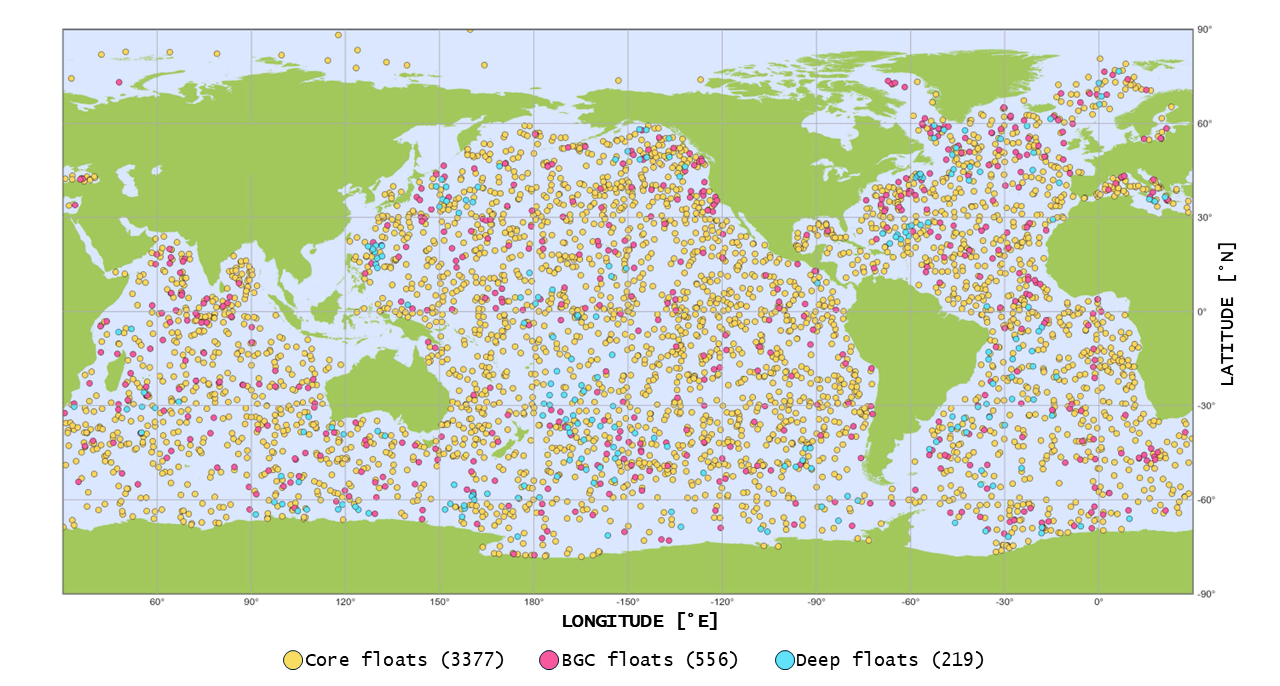
\includegraphics[width=16.0 cm]{figures/fig1.1.png}
    \caption{Global spatial distribution of Argo float deployments as of March 2025. The network includes three main types of profiling floats: Core floats, which measure temperature, salinity, and pressure in the upper 2000 m of the ocean; biogeochemical (BGC) floats, which are additionally equipped with sensors to observe variables such as dissolved oxygen, acidity, nitrate, and chlorophyll; and Deep floats, designed to extend observations to depths greater than 2000 m, reaching up to 4000-6000 m depending on the platform. The numbers in parentheses indicate the total number of active floats of each type. \emph{Source: adapted from \textcite{thierry2025advancing}}.}
    \label{fig:argo_1.1}
\end{figure}

\emph{Expendable bathythermograph (XBT) probes}

XBTs are widely used oceanographic instruments that provide vertical profiles of seawater temperature. Measurements are obtained through a thermistor embedded in a free-falling probe, while depth is estimated indirectly from a fall-rate equation rather than measured directly \parencite{simoncelli2024reprocessing}. The probe is not recovered after deployment.

\emph{Research vessels}

Despite being large and resource-intensive platforms, research vessels are highly specialized for oceanographic applications. They enable the collection of water samples for biogeochemical analysis and the deployment of complex and heavy instrumentation \parencite{satterthwaite2025essential}. While they remain fundamental to ocean research, ship-based observations are typically episodic and campaign-based rather than continuously operational.

\emph{Gliders and autonomous underwater vehicles (AUVs)}

Underwater gliders and AUVs are mobile robotic platforms designed to follow predefined mission trajectories and collect oceanographic data. AUVs use propeller-based propulsion systems that enable active control of their movement \parencite{sahoo2019advancements}, whereas gliders rely on buoyancy-driven motion combined with hydrodynamic lift generated by wings \parencite{wang2025development}. These platforms typically perform repeated vertical profiles, following a sawtooth trajectory, to acquire measurements of physical and, in some cases, biogeochemical variables throughout the water column. Despite their versatility, their operation is constrained by factors such as energy consumption, endurance, and depth limitations.

\emph{Commercial or non-research vessels}

Ship-based observing systems, including Ships of Opportunity (SOOP) and Volunteer Observing Ships (VOS), rely primarily on commercial vessels equipped with sensors to collect oceanographic and atmospheric data during routine operations. These platforms provide cost-effective observations with broad spatial coverage and play a key role in sustaining operational XBT deployments \parencite{haris2021sounding, jiang2019enhancing}. However, their sampling is often constrained by predefined shipping routes, which may not coincide with regions of specific scientific interest.

\emph{Moorings}

Moorings are typically fixed platforms equipped with multiple sensors that provide high temporal resolution time series of a wide range of oceanographic properties. They can collect measurements throughout the water column at a fixed location, as well as atmospheric variables at the surface. In addition to physical parameters, moorings can be instrumented to measure biogeochemical variables such as oxygen, carbon dioxide, and chlorophyll \parencite{bailey2019coastal}. Due to their relatively high installation and maintenance costs, moorings are deployed in limited numbers and are generally located in regions of particular scientific or operational interest.

\emph{High-frequency radar (HFR)}

HFR systems, typically installed along coastlines, provide measurements of water level and sea surface currents with high spatial and temporal resolution. Although based on electromagnetic wave scattering, they are generally considered part of the coastal \emph{in situ} observing infrastructure due to their fixed, land-based deployment and continuous monitoring capability \parencite{serafy2023eurogoos}. These systems deliver near-real-time information over coastal areas and are widely used in operational applications such as coastal management, including pollutant transport monitoring and marine safety \parencite{payandeh2023occurrence, serafy2023eurogoos}. Despite their relatively limited spatial coverage compared to satellite observations, they offer detailed observations of surface circulation in coastal regions.

The second primary method to collect ocean data is remote sensing. Although the sensors are located far from the data source, satellite-based observations have become essential for operational ocean monitoring, as they provide near-real-time information on key ocean surface properties. Since their widespread adoption in the 1980s, satellite observations have contributed significantly to advancing oceanographic knowledge, enabling the discovery and characterization of previously unresolved ocean processes \parencite{robinson2010introduction}. One of the main advantages of remote sensing is its extensive spatial coverage, allowing observations from regional to global scales and providing consistent, repeated measurements across space and time, which are often not achievable with traditional \emph{in situ} sampling methods \parencite{avouris2025advancements}. The high temporal resolution and the long-term accumulation of satellite datasets has proven fundamental for assessing ocean variability, identifying trends, and analyzing the occurrence of extreme events.

Satellite remote sensing relies on measuring the different types of electromagnetic radiation reflected by the ocean surface. Optical measurements of reflected radiation are used to derive variables such as chlorophyll-\emph{a} concentration, turbidity, suspended particulate matter, and water clarity \parencite{topp2020research}. In addition, other satellite techniques allow the estimation of key physical variables, such as sea surface temperature (SST) and sea surface height (SSH). SST is estimated from the relationship between temperature and the thermal radiation emitted by the ocean surface, measured in infrared or microwave wavelengths \parencite{minnett2019half}. Because the atmosphere alters this signal, correction algorithms are applied, and only cloud-free measurements are typically used to ensure accurate SST estimates. In contrast, SSH is measured using radar altimetry, which determines the distance between the satellite and the ocean surface by timing how long a microwave pulse takes to travel to the sea surface and back \parencite{srinivasan2023satellite}. Simultaneously, the satellite's precise position in space is calculated using tracking systems. By combining these two measurements, the height of the sea surface relative to a reference level can be accurately estimated

Satellite data products are distributed in different processing levels, which reflect the degree of transformation applied to the original measurements \parencite{robinson2010methods}. Level 0 (L0) corresponds to raw data in binary form, containing unprocessed sensor readings. Level 1 (L1) products consist of calibrated, multi-channel signals organized in the original scan-line coordinates of the sensor. Level 2 (L2) products are geolocated ocean data, in which the measurements are mapped to specific positions on the Earth's surface and converted into geophysical variables. Level 3 (L3) datasets are obtained by mapping and interpolating L2 products onto regular spatial grids, typically covering regional to global domains. Finally, Level 4 (L4) products represent fully processed, gap-filled, and analyzed gridded datasets, often generated by combining multiple data sources and applying interpolation or DA techniques to provide continuous fields. The higher-level products, particularly L3 and L4 datasets, are user-oriented products routinely distributed in operational contexts (e.g., L3 products \parencite{eucmems2019slal3, eucmems2022sstl3}; L4 products \parencite{eucmems2019slal4, eucmems2019ho}), and are widely used to support ocean monitoring and forecasting applications.

In operational oceanography, no single observation method is sufficient to fully characterize the ocean state. Remote sensing and \emph{in situ} observations are complementary techniques, both within and across observing systems, and their combined use is essential to overcome the inherent limitations of each approach. By integrating multiple observation platforms, it is possible to improve spatial and temporal coverage, thereby enhancing the quality and consistency of ocean datasets \parencite{lin2020ocean}. Moreover, the availability of independent measurements of the same variable enables cross-calibration and validation of both sensors and numerical models, which are fundamental components of operational forecasting systems \parencite{schiller2018overview}. Within this context, the effective combination of heterogeneous observational data sources becomes a central requirement for advancing ocean monitoring and prediction capabilities.

\section{Ocean models and the MOHID\\Modelling System}
Ocean modelling constitutes the second fundamental component of operational oceanography, complementing observing systems by providing a dynamic and predictive representation of the marine environment. In this context, a numerical model can be understood as a mathematical representation of physical processes, where the governing equations describe the dynamics of ocean circulation and associated phenomena. Once these equations are defined, they are discretized using numerical methods and implemented as computational algorithms that allow the ocean state to be advanced in time. In the following chapters, the MOHID Modelling System is used as the core numerical tool; however, its characteristics are only briefly introduced. For this reason, a more formal description of the modelling approach is provided in this section, focusing on the fundamental principles and equations underlying the MOHID system.

The mathematical formulation of ocean dynamics is based on a system of differential equations derived from the fundamental conservation principles of physics, including the conservation of mass, momentum, and energy \parencite{kampf2009ocean}. In MOHID, the solution of these equations is approximated using an Eulerian model, in which the conservation of physical properties is evaluated within fixed regions of space, referred to as control volumes (CVs), while water flows through them. Accordingly, the governing equations are discretized in space, allowing them to be solved independently within each CV that composes the domain of interest. MOHID applies the finite volume method \parencite{martins1998three}, in which each CV corresponds to a cell of the computational mesh. The spatial resolution of the model is therefore determined by the size and number of these cells: higher-resolution configurations use a greater number of smaller cells to represent the same domain. Although this leads to a more detailed representation of ocean processes, it also significantly increases the computational cost, as the governing equations must be solved for each individual cell, a limitation inherent to numerical discretization \parencite{tang2021modeling}.

The governing equations can be derived from the general transport equation, which, for an infinitesimal cubic control volume defined in a Cartesian coordinate system, is expressed by \bCref{eq:cp1_transport} \parencite{versteeg2007introduction, kampf2009ocean}:

\begin{equation} \label{eq:cp1_transport}
\begin{aligned}
    \frac{\partial(\rho\phi)}{\partial t}
    + \frac{\partial(\rho\phi u)}{\partial x}
    + \frac{\partial(\rho\phi v)}{\partial y}
    + \frac{\partial(\rho\phi w)}{\partial z} = \\
    \frac{\partial(\rho\phi)}{\partial t}
    + \nabla \cdot (\rho\phi \mathbf{u}) = 
    \sum \left( \text{Sources} - \text{Sinks} \right)
\end{aligned}
\end{equation}

where $\rho$ represents the fluid density, $\phi$ is a generic scalar property of the fluid, and $\mathbf{u} = (u, v, w)$ is the velocity vector in the Cartesian coordinate system $(x, y, z)$. The first term represents the temporal ($t$) rate of change of $\phi$ within the CV, while the second term describes the divergence of the advective flux, accounting for its transport by the fluid motion. The right-hand side term represents the contribution of internal processes that cause variations in $\phi$ within the CV, such as physical, chemical, or biological interactions. Depending on the choice of $\phi$, \bCref{eq:cp1_transport} can be used to derive the governing equations for different variables, such as the conservation of mass (continuity equation in \bref{eq:cp1_mass}), and the conservation of momentum along the three axis (\textbf{Equations} \bref{eq:cp1_momentumx} to \bref{eq:cp1_momentumz}):

\begin{equation}\label{eq:cp1_mass}
    \frac{\partial(\rho)}{\partial t} + \nabla \cdot (\rho \mathbf{u}) = 0,
\end{equation}

\begin{equation}\label{eq:cp1_momentumx}
    \frac{\partial(\rho u)}{\partial t} + \nabla \cdot (\rho u \mathbf{u}) = \sum F_{x},
\end{equation}

\begin{equation}\label{eq:cp1_momentumy}
    \frac{\partial(\rho v)}{\partial t} + \nabla \cdot (\rho v \mathbf{u}) = \sum F_{y},
\end{equation}

\begin{equation}\label{eq:cp1_momentumz}
    \frac{\partial(\rho w)}{\partial t} + \nabla \cdot (\rho w \mathbf{u}) = \sum F_{z},
\end{equation}

where $\sum F$ represents the sum of forces acting on a fluid particle, responsible for changes in its motion along the $x$, $y$, and $z$ directions.

In MOHID, the previous governing equations are applied at a macroscopic level to the CV of each grid cell. The model considers the flow to be incompressible, while assuming the hydrostatic equilibrium and Boussinesq approximation. In such manner, the equations become \parencite{martins1998three}:

\begin{equation}\label{eq:cp1_massmohid}
    \frac{\partial u}{\partial x} + \frac{\partial v}{\partial y} + \frac{\partial w}{\partial z} = \nabla \cdot \mathbf{u} = 0,
\end{equation}

\begin{equation}\label{eq:cp1_momentumxmohid}
\begin{aligned}
    \frac{\partial u}{\partial t}
    + \nabla \cdot (\mathbf{u}u)
    &= fv
    - g\frac{\rho_{\eta}}{\rho_0} \frac{\partial \eta}{\partial x}
    - \frac{1}{\rho_0}\frac{\partial p_s}{\partial x}
    - \frac{g}{\rho_0} \int_{Z}^{\eta}\frac{\partial \rho'}{\partial x} dz \\
    &\quad + \frac{\partial}{\partial x}\left( A_h \frac{\partial u}{\partial x}\right)
    + \frac{\partial}{\partial y}\left( A_h \frac{\partial u}{\partial y}\right)
    + \frac{\partial}{\partial z}\left( A_v \frac{\partial u}{\partial z}\right)
\end{aligned}
\end{equation}

\begin{equation}\label{eq:cp1_momentumymohid}
\begin{aligned}
    \frac{\partial v}{\partial t}
    + \nabla \cdot (\mathbf{u}v)
    &= -fu
    - g\frac{\rho_{\eta}}{\rho_0} \frac{\partial \eta}{\partial y}
    - \frac{1}{\rho_0}\frac{\partial p_s}{\partial y}
    - \frac{g}{\rho_0} \int_{Z}^{\eta}\frac{\partial \rho'}{\partial y} dz \\
    &\quad + \frac{\partial}{\partial x}\left( A_h \frac{\partial v}{\partial x}\right)
    + \frac{\partial}{\partial y}\left( A_h \frac{\partial v}{\partial y}\right)
    + \frac{\partial}{\partial z}\left( A_v \frac{\partial v}{\partial z}\right),
\end{aligned}
\end{equation}

\begin{equation}\label{eq:cp1_momentumzmohid}
    \frac{\partial p}{\partial z} = - \rho g,
\end{equation}

where $(u,v,w)$ are the components of the velocity vector $\mathbf{u}$ in the Cartesian coordinate system $(x,y,z)$, and $\eta$ is the free-surface elevation. On the right-hand side of \textbf{Equations}~\bref{eq:cp1_momentumxmohid} and~\bref{eq:cp1_momentumymohid}, the first term represents the Coriolis force per unit mass with parameter $f$. The second term represents the barotropic pressure-gradient force associated with gradients in the free-surface elevation, where $\rho_{\eta}$ is the density at the free surface and $\rho_0$ is a reference density. The third term represents the barotropic pressure-gradient force associated with atmospheric pressure gradients, where $p_s$ is the surface atmospheric pressure. The fourth term represents the baroclinic pressure-gradient force, computed from the vertical integral of the horizontal density gradients, where $\rho'$ is the density anomaly, such that $\rho = \rho_0 + \rho'$. The remaining terms represent diffusive (turbulent stress) forces per unit mass, where $A_h$ and $A_v$ are the horizontal and vertical turbulent viscosity coefficients, respectively. \bCref{eq:cp1_massmohid} is the continuity equation (mass conservation) under the incompressibility condition, while \bCref{eq:cp1_momentumzmohid} corresponds to the vertical momentum equation under the hydrostatic approximation, in which vertical accelerations are neglected and the pressure gradient is balanced by gravity. For a more detailed description of the numerical implementation and discretization methodology adopted in MOHID, the reader is referred to \textcite{martins1998three}.

Beyond its numerical formulation, MOHID stands out for its versatility and wide range of applications. The model adopts a generic vertical discretization, allowing the definition of multiple vertical subdomains, which facilitates the accurate representation of complex bathymetries and stratified flows. In addition, MOHID includes a Lagrangian model component capable of simulating the transport of particles \parencite{braunschweig2004object}, which has proven particularly useful for applications such as marine litter dispersion and oil spill tracking. The system is also highly comprehensive in terms of physical and biogeochemical processes, incorporating modules that simulate not only hydrodynamic variables such as temperature and salinity, but also ecosystem-related components \parencite{neves2007numerical}, including phytoplankton, zooplankton, bacteria, nutrients (e.g., nitrogen and phosphorus), and dissolved oxygen. Owing to these features, MOHID has been successfully applied in a wide range of studies and applications, including sediment transport \parencite{monreal2025sediment}, marine litter \parencite{rosas2021marine}, microplastics \parencite{cloux2024regional}, oil spills \parencite{mittal2024oil}, wave-current interactions through coupling with the SWAN model \parencite{mills2025evaluating}, and nutrient flux analyses \parencite{pablo2022climatology}, among many others.

\section{Motivation and Objectives}
In recent decades, the amount of oceanographic data has increased significantly, driven by the expansion of satellite missions, \emph{in situ} observation networks, and autonomous platforms. However, despite these advances, ocean observation still presents persistent important limitations, including gaps in spatial and temporal coverage, as well as difficulties in resolving fine-scale processes \parencite{tzachor2023}. On the other hand, numerical models provide a continuous representation of the ocean but remain an approximation of reality and are therefore subject to errors and uncertainties \parencite{evensen2022data}. In this context, DA methodologies play a fundamental role by allowing the combination of observations and model outputs in a consistent way, thereby mitigating the aforementioned limitations.

Beyond improving the estimation of the ocean state, DA systems can also be used to support the design and optimization of observing systems, including the development of new observation strategies. This is exactly the purpose of Observing System Simulation Experiments (OSSEs), which provide a controlled numerical framework to evaluate the impact of different observation strategies on model performance \parencite{halliwell2014Rigorous, halliwell2015osse}. In an OSSE, a reference simulation is assumed to represent the ocean true state, from which synthetic observations are extracted. These observations are then assimilated into an independent model integration, allowing the assessment of how their availability, type, and distribution influence the accuracy of the system when assessed against this reference. Through this approach, OSSEs enable the systematic evaluation of observing strategies prior to their real-world implementation, providing a valuable tool to optimize observation networks and improve forecasting capabilities.

In the Algarve region, oceanographic observations remain particularly limited and fragmented. Although measurements have been collected over the years, \emph{in situ} data are predominantly research-driven and campaign-based, typically designed to address specific scientific questions rather than to support sustained operational monitoring (e.g., \textcite{rautenbach2024, oliveira2024, garel2016characterisation}). As a result, these datasets are characterized by significant temporal discontinuities and limited spatial coverage. Furthermore, the available observations are often distributed across different institutions and projects, lacking integration within a unified observing system. These limitations reduce their effectiveness for continuous monitoring and forecasting applications, highlighting the need for more coordinated and efficient observation strategies. From this perspective, different initiatives aim at advancing ocean observation in European seas, such as the Horizon 2020 NAUTILOS project \parencite{novellino2022new}, which focus on the development of innovative and cost-effective technologies to support operational monitoring. The work presented in this thesis has benefited from its close connection with this project.

In light of the previous discussion, this work aims to research the integration of DA methodologies into coastal ocean models, with the purpose of establishing the foundations of a modern DA system linked to the existent Algarve Operational Modelling and Monitoring System (SOMA) \parencite{cima2024soma}. The incorporation of a DA method is expected to enhance the accuracy of model forecasts and to support the development of advanced oceanographic products for the region. This objective aligns with the strategic plan of the Centre for Marine and Environmental Research (CIMA) of the University of Algarve, supporting the research domain of \emph{Ocean and Coastal Dynamics}. To achieve this general goal, the specific objectives of this work are:

\begin{itemize}
    \item To adapt a DA method based on the Ensemble Optimal Interpolation (EnOI) scheme to SOMA;
    
    \item To design and implement an OSSE system for SOMA, enabling the systematic evaluation and optimization of observation strategies, particularly for low-cost sensors, while maintaining flexibility for applications beyond this initiative;
    
    \item To develop an operational structure for SOMA capable of supporting routine forecast production and providing a foundation for the future integration of DA processes, thereby improving model reliability and operational efficiency.
\end{itemize}

\subsection*{Thesis structure}

This thesis follows a manuscript-based format, in which each of the following chapters corresponds to a published or submitted scientific article. Although the chapters may share common elements, such as the the modelling and OSSE systems, they address distinct research questions and are therefore presented as independent manuscripts. In this manner, they are included in a form closely aligned with the original publications, with only minor adjustments to formatting. All bibliographic references cited throughout the thesis are compiled into a single bibliography section at the end of the document. The full citation for each chapter is provided on its respective title page and is also listed below:

\begin{itemize}
    \item \bCref{sec:cp2}: Mendonça, F., Martins, F., \& Bertino, L. (2025). Design of an Observing System Simulation Experiment for the Operational Model of the Southwestern Coast of Iberia (SOMA). \textit{Journal of Marine Science and Engineering}, 13(9), 1830. \href{https://doi.org/10.3390/jmse13091830}{https://doi.org/10.3390/jmse13091830}.

    \item \bCref{sec:cp3}: Mendonça, F., Martins, F. \& Bertino, L. (2026). Optimizing Coastal Observation Strategies for a Southwestern Iberian Forecasting System Using Observing System Simulation Experiments. Submitted to \href{https://www.frontiersin.org/journals/marine-science}{Frontiers in Marine Science} (Electronic ISSN 2296-7745) and currently under review.
    
    \item \bCref{sec:cp4}: Mendonça, F., Martins, F., \& Janeiro, J. (2023). SMS-Coastal, a New Python Tool to Manage MOHID-Based Coastal Operational Models. \textit{Journal of Marine Science and Engineering}, 11(8), 1606. \href{https://doi.org/10.3390/jmse11081606}{https://doi.org/10.3390/jmse11081606}.
\end{itemize}

Each of the aforementioned chapters can be summarized as follows. \bCref{sec:cp2}, which can be regarded as the methodological core of this thesis, introduces the OSSE system tailored for the SOMA model. It defines the OSSE concept, presents the general formulation of the Ensemble Optimal Interpolation (EnOI) method as the DA scheme, and describes the main design aspects adopted in the SOMA OSSE system. \bCref{sec:cp3} focuses on the application of the developed system, presenting the use of the SOMA OSSE system to evaluate different observation strategies within the model domain. The impact of these strategies on forecast performance is assessed, providing guidance on the optimal placement, number, and type of sensors to be deployed, in future observational initiatives. \bCref{sec:cp4} presents SMS-Coastal, a generic application designed to operationalize SOMA and other MOHID-based models. This tool provides the operational infrastructure required to support forecasting systems and establishes a foundation for the future integration of DA processes. Finally, \bCref{sec:cp5} summarizes the main conclusions of the thesis, integrating the results of the individual chapters and outlining perspectives for future developments.

\chapter{Design of an Observing System Simulation Experiment for the Operational Model of the Southwestern Coast of Iberia (SOMA)} \label{sec:cp2}
\vspace{\fill}
\textbf{Article reference}:\\
Mendonça, F., Martins, F., \& Bertino, L. (2025). Design of an Observing System Simulation Experiment for the Operational Model of the Southwestern Coast of Iberia (SOMA). \textit{Journal of Marine Science and Engineering}, 13(9), 1830. \href{https://doi.org/10.3390/jmse13091830}{https://doi.org/10.3390/jmse13\\091830}
\newpage

\section{Abstract}
Observing System Simulation Experiments (OSSEs) provide a framework in which to evaluate the impact of prospective ocean-observation networks on model forecasting performance prior to their actual deployment. This study presents the design and validation of an OSSE tailored for the operational coastal model of southern Portugal, SOMA. The system adopts the fraternal twins approach and a univariate data-assimilation scheme based on Ensemble Optimal Interpolation to update the model's 3D temperature structure with SST. The methodology provides a flexible framework that preserves the statistical structure of real observation errors while remaining independent of SOMA. This allows straightforward transfer to other applications, thereby broadening its applicability and making it useful as a starting point in the design of observation networks beyond that presented in this case study. The OSSE experiments were compared against corresponding Observing System Experiments (OSEs) using real satellite SST products. Results show that the designed OSSE is internally consistent, sensitive to observation density, and capable of reproducing realistic correction patterns that closely match those obtained in the OSEs. These findings provide strong evidence that the SOMA OSSE system is a reliable tool for assessing the potential impact of future surface-observation strategies.

\vspace{15mm}
\noindent\textbf{Keywords}: coastal model; ocean observation; data assimilation; ensemble optimal interpolation; observation experiments
\vspace{10mm}

\section{Introduction} \label{sec:ossedesign_intro}
Numerical modelling is one of the primary tools used for understanding and predicting marine system dynamics. Hydrodynamic models simulate the ocean state by translating the physics of fluid motion into a computational framework that approximates the solution of discretized primitive equations using numerical methods \parencite{versteeg2007introduction, griffies2006some}. These methods are implemented as algorithms that advance the ocean state forward in time over a defined spatial domain. Through this process, models enable the simulation of oceanic conditions, providing valuable insights into the structure and evolution of marine systems under both natural variability and anthropogenic influence.

While numerical models are essential in ocean prediction, they are still only one element of the broader framework used to understand marine systems in operational oceanography. Observations lie at the centre of the scientific method and provide the factual basis needed to develop and validate theoretical formulations and numerical models. It is primarily through the continuous and systematic observation of ocean phenomena via in-situ measurements, remote sensing, or other monitoring technologies \parencite{letraon2011satellites} that empirical knowledge of the ocean's dynamics is established. Historical data collected on water variables provide critical information about climate evolution, such as changes in sea surface height (SSH) \parencite{frederikse2020causes, gomez2024satellite} and variations in water temperature \parencite{mills2024baseline, liu2023twenty}.

The observation network is a cornerstone of operational oceanography and has driven increasing demand for high-quality oceanographic data. As a result, the evolution of observation-system technologies has enabled real-time measurements of various ocean variables \parencite{legler2015current, letraon2015use}. Despite this progress, observational data often present significant spatial and temporal gaps, particularly in remote or logistically challenging regions. Because the implementation of new ocean-observation systems typically involves substantial financial investment and technical complexity, Observing System Simulation Experiments (OSSEs) provide a framework in which to evaluate the potential impact of additional observations before their actual deployment by exploring hydrodynamic models and data assimilation (DA) systems \parencite{prive2023robustness}.

The purpose of an OSSE system is to ensure that the additional observations will meaningfully contribute to scientific and operational goals. However, since it relies on synthetic data (Section 3), the development of such a system requires using an Observing System Experiment (OSE) to serve as a benchmark by which to validate the OSSE \parencite{halliwell2014Rigorous}. While both approaches operate in a similar manner, OSEs rely on real-world, existing observations to evaluate their impact through data denial experiments, comparing model performance with and without specific datasets. Demonstrating that an OSSE system produces impact assessments consistent with those of an OSE, researchers confirm the credibility of the framework for evaluating future observing systems. This validation step is critical to ensuring the system produces realistic and reliable predictions before resources are committed to new observational deployments.

Within this context, the NAUTILOS project \parencite{novellino2022new} is focused on developing cost-effective next-generation technologies for ocean observation. Funded by the Horizon 2020 program of the EU's Future of Seas and Oceans Flagship Initiative, the project addresses critical gaps in marine monitoring, particularly for chemical, biological, and deep-ocean physical variables. By integrating innovative sensors and samplers into a range of ocean platforms, such as autonomous vehicles, mooring buoys, and fisheries-observation systems, the project contributes to a standardized, interoperable system for marine data collection, enhancing global efforts to understand and manage ocean ecosystems. Aligned with the broader goals of the NAUTILOS project, the present work focuses on the development and validation of an OSSE system tailored to an operational hydrodynamic model of the southern coast of Portugal. The primary objective is to establish and verify the functionality of the OSSE system itself, ensuring that it is capable of supporting future assessments of observational strategies.

The subsequent sections are structured to present the key components and methodologies adopted in the development of the proposed OSSE system. Section \ref{sec:ossedesign_algarve} outlines the main oceanographic features of the Algarve region, the focus of this study. Next, Section \ref{sec:ossedesign_osse} provides a comprehensive overview of the OSSE framework, while Section \ref{sec:ossedesign_da} presents the general formulation of the Ensemble Optimal Interpolation (EnOI) scheme, which was used as the DA method in the designed system. Building on this context, the OSSE system was implemented for the Algarve Operational Modeling and Monitoring System (SOMA), a hydrodynamic model based on MOHID, as described in the first part of the methodology (Section \ref{sec:ossedesign_method}). The second part details the design choices made for the system, including a fraternal twins configuration of SOMA, which was used to represent two distinct model realizations for comparative assessment. It also describes how observations are extracted from the system and the implementation of the EnOI scheme in SOMA. Finally, Section \ref{sec:ossedesign_results} and Section \ref{sec:ossedesign_conclude} present the results of the system's implementation and the main conclusions of this work.

\section{Algarve General Circulation} \label{sec:ossedesign_algarve}
The south of Iberia is characterized by a Mediterranean climate, which features distinct seasonal variations with hot, dry summers and mild, humid winters. The average annual temperature in this region is approximately 17$^\circ$C, with summer temperatures frequently exceeding 22$^\circ$C and reaching maximums around 40$^\circ$C. In contrast, winter temperatures typically remain below 18$^\circ$C, rarely dropping below freezing \parencite{beck2018present}. The climate and especially the wind regime on the Algarve coast are intimately related to the North Atlantic Oscillation (NAO) \parencite{leitao2018northerly, hurrell2010north}. During the warmest months, the effects of NAO combined with the low precipitation rate can even cause extreme droughts \parencite{dias2020intefrating, santos2010spatial}. In the summer, it is common for the NAO pressure gradient to be large, favouring strong westerly winds in northern Europe. However, as the centre of the high-pressure field moves towards Portugal, the winds change direction, becoming northerly on the west coast. In winter, on the other hand, this gradient is not so noticeable and the wind patterns are more variable, and northerly winds are generally weaker or even replaced by southerly components \parencite{fiuza1982climatological}.

The observed oceanographic patterns and circulation in the Algarve are highly dynamic and are influenced by a combination of upwelling, poleward currents, and mesoscale eddies \parencite{relvas2002mesoscale}. Based on the cyclical wind regimes associated with the pressure-gradient variability of NAO, the southward winds in the summer drive upwelling currents along the west coast, bringing cold, nutrient-rich waters to the surface \parencite{relvas2007physical}. During that season, the temperature difference between land and ocean waters creates a pressure gradient that channels the northerly winds along the south coast, creating conditions that favour upwelling currents in this region as well \parencite{leitao2018northerly}. As a result of the upwelling, the flow of colder waters along the Algarve's southern coastline is typically eastward, while warmer oceanic waters lying offshore of the continental shelf flow westward \parencite{fiuza1983upwelling}.

When the NAO pressure gradient weakens, westerly winds become predominant, a typical condition of winter months. This change reduces the intensity of upwelling events, thereby allowing the warm countercurrent from the Gulf of Cadiz to strengthen and propagate westward along the south coast \parencite{telesmachado2007onset, garel2016characterisation}. This current continues in a poleward course along the west coast, carrying warm and saline waters that interact with other equatorward currents and thus creating complex circulation patterns along the Portuguese coastline \parencite{haynes1990poleward, frouin1990observations}. Although upwelling is possible during the cold season, it is driven by this poleward flow and differs from the upwelling seen in summer, which is characterized by colder and nutrient-rich waters \parencite{relvas2005separated}. In this context, the most relevant variable to update in the model for this region would be sea surface temperature (SST), as its inclusion would help to constrain and correct the vertical structure of the coastal water masses, thereby improving the representation of subsurface temperature fields.

\section{Observation System Simulation Experiment} \label{sec:ossedesign_osse}
Driven by the need to mitigate spatial and temporal gaps in ocean data coverage, observation networks are continuously being developed and improved. As technological advancements enable the deployment of increasingly sophisticated sensors and platforms, it becomes essential to evaluate their potential impact to ensure they will bring benefits to ocean forecasting once operational. This is the exact purpose of an OSSE system, which provides a framework in which to assess observation networks prior to their real-world deployment, helping to guide resource allocation and optimize the network design.

OSSE systems have been employed in numerical weather prediction since the early 1980s \parencite{atlas1985impact, atlas1997atmospheric}. This methodology was adopted by the ocean-modelling community more recently \parencite{mourre2006relative, oke2007impact}, and due to this, oceanic OSSEs remain in a relatively early stage of development compared to their atmospheric counterparts. As discussed in \parencite{halliwell2014Rigorous}, this highlights the importance of adopting methodical and robust design strategies, as well as rigorous validation techniques. Without proper calibration, OSSE systems risk producing misleading results, potentially overestimating or underestimating the value of proposed observational systems and thus supporting biased decision-making in sensor deployment.

The essential concept behind an OSSE is the substitution of reality, which is difficult and expensive to observe, with a high-quality numerical simulation, or, as it is commonly referred to, the Nature Run (NR). The NR serves as a proxy for the true state of the ocean, and synthetic observations are extracted from the simulation. In parallel, a Forecast Model (FM) is integrated and has its state updated with the synthetic observations using a DA system. This process constitutes an OSSE. The performance of the FM and OSSE forecasts are then assessed against the NR using a set of defined metrics and parameters. Essentially, OSSEs function as “data denial” experiments, creating conditions in which to assess the effectiveness of different observation strategies by selectively manipulating synthetic data.

As highlighted in \parencite{halliwell2014Rigorous, halliwell2015osse}, the numerical frameworks behind NR and FM should be as distinct as possible; i.e., the two models should have different numerical implementations, resolution grids, parameterisations, and boundary conditions. However, achieving this level of difference between the NR and FM can be challenging. Consequently, one might want to create an OSSE system in which NR and FM are based on the same numerical model (e.g., \textcite{ford2021assimilating} and \textcite{fennel2022ocean}) but adjust other factors to the greatest extent possible. These systems are referred to as fraternal twins experiments: the same model is used, but with different setups. In contrast, in an identical twins approach, i.e., one in which NR and FM are based on the same model and the differences between them are too limited, the experiment leads to unrealistic error growth between the models, yielding biased impact assessments in ocean DA systems \parencite{yu2019evaluation}.

As mentioned in Section \ref{sec:ossedesign_intro}, prior to employing an OSSE system for the evaluation of a prospective observation system, it is of paramount importance to validate the system with a corresponding OSE. An OSE functions in a manner analogous to an OSSE, but it employs actual observations instead of the synthetic data generated by the NR. Thus, the FM is assessed against actual observations in the OSE, whereas in the OSSE, it is compared to the NR. When designing an OSSE, it is crucial to ensure that the differences between the NR and FM are substantial but not so extensive that the latter becomes unrealistic. Furthermore, special attention must be paid to avoid assigning unrealistic errors to the synthetic observations, as this could skew impact assessments. Once these steps are completed, the consistency of observation impacts between the two systems is compared. The common metrics used to assess observations in both the OSE and OSSE, such as averages, root mean square errors (RMSE), and skill scores, are detailed in Section \ref{sec:ossedesign_appxA}.

\section{Data-Assimilation Scheme} \label{sec:ossedesign_da}
An ocean model is a representation of reality and is therefore prone to imperfection. The states generated by a model are subject to various sources of uncertainty, including mathematical model simplifications, model parameterisation, limited temporal and spatial resolution, truncation and rounding errors, and boundary and initial conditions. DA methodologies provide a set of processes to reduce these uncertainties by combining real-world measurements with model results. They aim to estimate the best state of the represented system by statistically evaluating the errors of both the observations and the model.

Advanced data-assimilation methods, such as the four-dimensional variational (4DVAR) or the Ensemble Kalman Filter (EnKF) methods, have been proven optimal for linear systems but are computationally expensive. In practice, most operational forecasting systems rely on computationally inexpensive variants like 3DVAR and the EnOI \parencite{martin2025data}. Regardless, most DA problems can be traced back to the Bayesian state-estimation problem, meaning each method derives from this common root but assumes different strategies and assumptions. Since a comprehensive review of DA methods lies beyond the scope of this paper, readers are directed to consult the formulations presented in \textcite{carrassi2018data} and \textcite{evensen2022data}, starting from the Bayesian formulation in both.

Given its similarities to methods employed in operational systems, the EnOI was selected for this work. This method builds on the EnKF framework, which estimates the background error covariance matrix with the spread and correlations among an ensemble of finite model realizations \parencite{evensen1994sequential}. During the analysis update, this approximation provides a representation of the error statistics for the ensemble average. However, ensemble-based DA methods like EnKF can be computationally prohibitive due to the cost of generating and integrating large ensembles \parencite{oke2010ocean}, a limitation that EnOI mitigates by using a static (time-invariant) ensemble.

The EnOI scheme can be regarded as a simplification of the EnKF \parencite{evensen2003ensemble, oke2002assimilaiton}. The main distinction lies in the assumption of the time-invariant error statistics: in EnOI, the background error covariance matrix is static in time and is derived from a fixed ensemble of model anomalies. As noted in \parencite{oke2010ocean}, because the computational cost of ensemble-based methods scales with the number of ensemble members, EnOI can be approximately N times less expensive than the EnKF, where N is the number of ensemble members used in both schemes. Moreover, in EnOI, the analysis update is computed only once for the background state, whereas in the EnKF, each ensemble member requires a separate update step. The general formulation of EnOI, including the standard analysis equation of a DA problem, is presented in Section \ref{sec:ossedesign_appxB}.

Although EnOI provides a computationally efficient alternative to EnKF by assuming a static background error covariance, it retains a key strength of ensemble-based methods: its multivariate assimilation capability. The background error covariance matrix encodes statistical relationships between different state variables, thereby allowing the update to propagate across them \parencite{counillon2009ensemble}. This feature enables the observation of a variable (e.g., SSH) to influence and modify other variables that are correlated (e.g., temperature and salinity), which is crucial for preserving dynamical consistency in ocean models. Due to its balance between computational efficiency and robust assimilation, EnOI has been widely adopted in various ocean applications, as seen in the above-mentioned studies: for shelf circulation off the Oregon (US) coast \parencite{oke2002assimilaiton}, using high-frequency (HF) radar-derived surface velocity measurements; for the Gulf of Mexico \parencite{counillon2009ensemble}, using satellite altimetry data; and in the Australian region \parencite{oke2010ocean}, using a combination of remote and in situ observations. It has also been used in other works, such as for the South Atlantic off the Brazilian coast \parencite{tanajura2013assimilation}, using satellite altimetry; for the western Mediterranean \parencite{lasheras2018dense}, using CTD probes and underwater glider datasets; and in the Hong Kong area \parencite{liu2021assimilation}, using temperature and salinity profiles.

\section{Methodology} \label{sec:ossedesign_method}
\subsection{The Operational Forecasting System of the Algarve}
To achieve the proposed objective of this work, the OSSE System was developed and integrated with the Algarve Operational Modelling and Monitoring System (SOMA) \parencite{janeiro2017integrating}. The aim is to provide a system that can be used to assess the impact of new observation networks launched in the region where the model is implemented and determine how the model's forecasting performance would benefit from these networks. The model itself is a realization of the MOHID Modelling System \parencite{sobrinho2021improving}, which is a robust numerical tool programmed in ANSI FORTRAN. It is designed in a modular architecture in which each module represents a different marine process that may be physical, chemical, or biological. Although the programming language is not specifically object-oriented, its architecture allows the model to work in this paradigm, which makes it possible to run several modules simultaneously, making it suitable for downscaling applications \parencite{braunschweig2004object} such as SOMA.

MOHID applies an Eulerian approach with a finite volume method for spatial discretization to solve the primitive Navier-Stokes equations of fluid motion. These equations, applied at a macroscopic level to the control volume of each grid cell, consist of the conservation of mass, the conservation of momentum, and a thermal energy equation. The model considers the assumptions of hydrostatic equilibrium and the Boussinesq approximation \parencite{mayeli2021buoyancy}. A notable feature of MOHID is its ability to use generic vertical coordinates, enabling the simulation of complex geometries across multiple vertical subdomains \parencite{martins2001modelling}. Temporal discretization is performed using a semi-implicit alternating-direction implicit (ADI) algorithm with two time levels per iteration \parencite{martins1998three, martins1999modelacao}. Additionally, the model includes modules for Lagrangian transport, which are particularly relevant for oil-spill applications \parencite{janeiro2014enhancing, moreira2023generic}.

According to \textcite{janeiro2012towards}, SOMA was initially developed as a high-resolution model designed to predict oil-spill trajectories off the Algarve coast. Subsequently, as demonstrated in \textcite{janeiro2017integrating}, it was further employed to identify sources of oil leakage by combining backtracking simulations with trajectory data from ships. Such studies confirmed SOMA's capability to reproduce the general ocean circulation in the Algarve region. As a result, the model was finally adjusted to render it operational; it has provided four-day daily forecasts since 2019, ensuring continuous oceanographic predictions of water conditions. The model has been evolving into an observatory for the region and features a visualization interface, with open access to the data available via a THREDDS server \parencite{cima2024soma}.

The model bathymetry is based on data from the European Marine Observation and Data Network (EMODNET) and is represented by two levels of increasing spatial resolution. The first level employs a horizontal grid with a resolution of 2 km, while the second level refines the grid to 1 km and is implemented in a smaller area. In both configurations, the vertical grid is discretized into 50 Cartesian layers, extending to a depth of about 4500 m. At the open boundary, a water-level condition based on the method proposed by \textcite{blumberg1985open} is applied, while a Flow Relaxation Scheme (FRS) \parencite{martinsen1987implementation} is used for the velocity, salinity, and temperature. FRS is also used to manage the communication between the two levels. Further details of the model implementation can be found in \textcite{janeiro2017integrating}. SOMA's implementation area is shown in \bCref{fig:batim_2.1}.

External boundary fields for current velocity, temperature, and salinity are provided by the Global Ocean Physics Analysis and Forecast, a product of Mercator Ocean International through the Copernicus Marine Environment Monitoring Service (CMEMS) \parencite{cmems2016mercator}. For the tide field, SOMA has an additional grid, which is a simple 2D hydrodynamic domain, forced by the FES2014 global tidal solution \parencite{carrere2013fes}. This domain has the single purpose of generating and supplying the tidal conditions to the first level of SOMA, and thus it is referred to as Level 0. At the atmospheric boundary, the model integrates data from the regional weather-forecast system SKIRON \parencite{kallos1997regional, papadopoulos2002weather}, which was developed by the Atmospheric Modeling and Weather Forecasting Group of the National and Kapodistrian University of Athens. The system provides hourly inputs on a 5 km resolution grid, including variables for wind-velocity components, air temperature, sea-level pressure, and other factors required to compute heat and momentum fluxes through bulk formulae.

\begin{figure}[H]
    \centering
    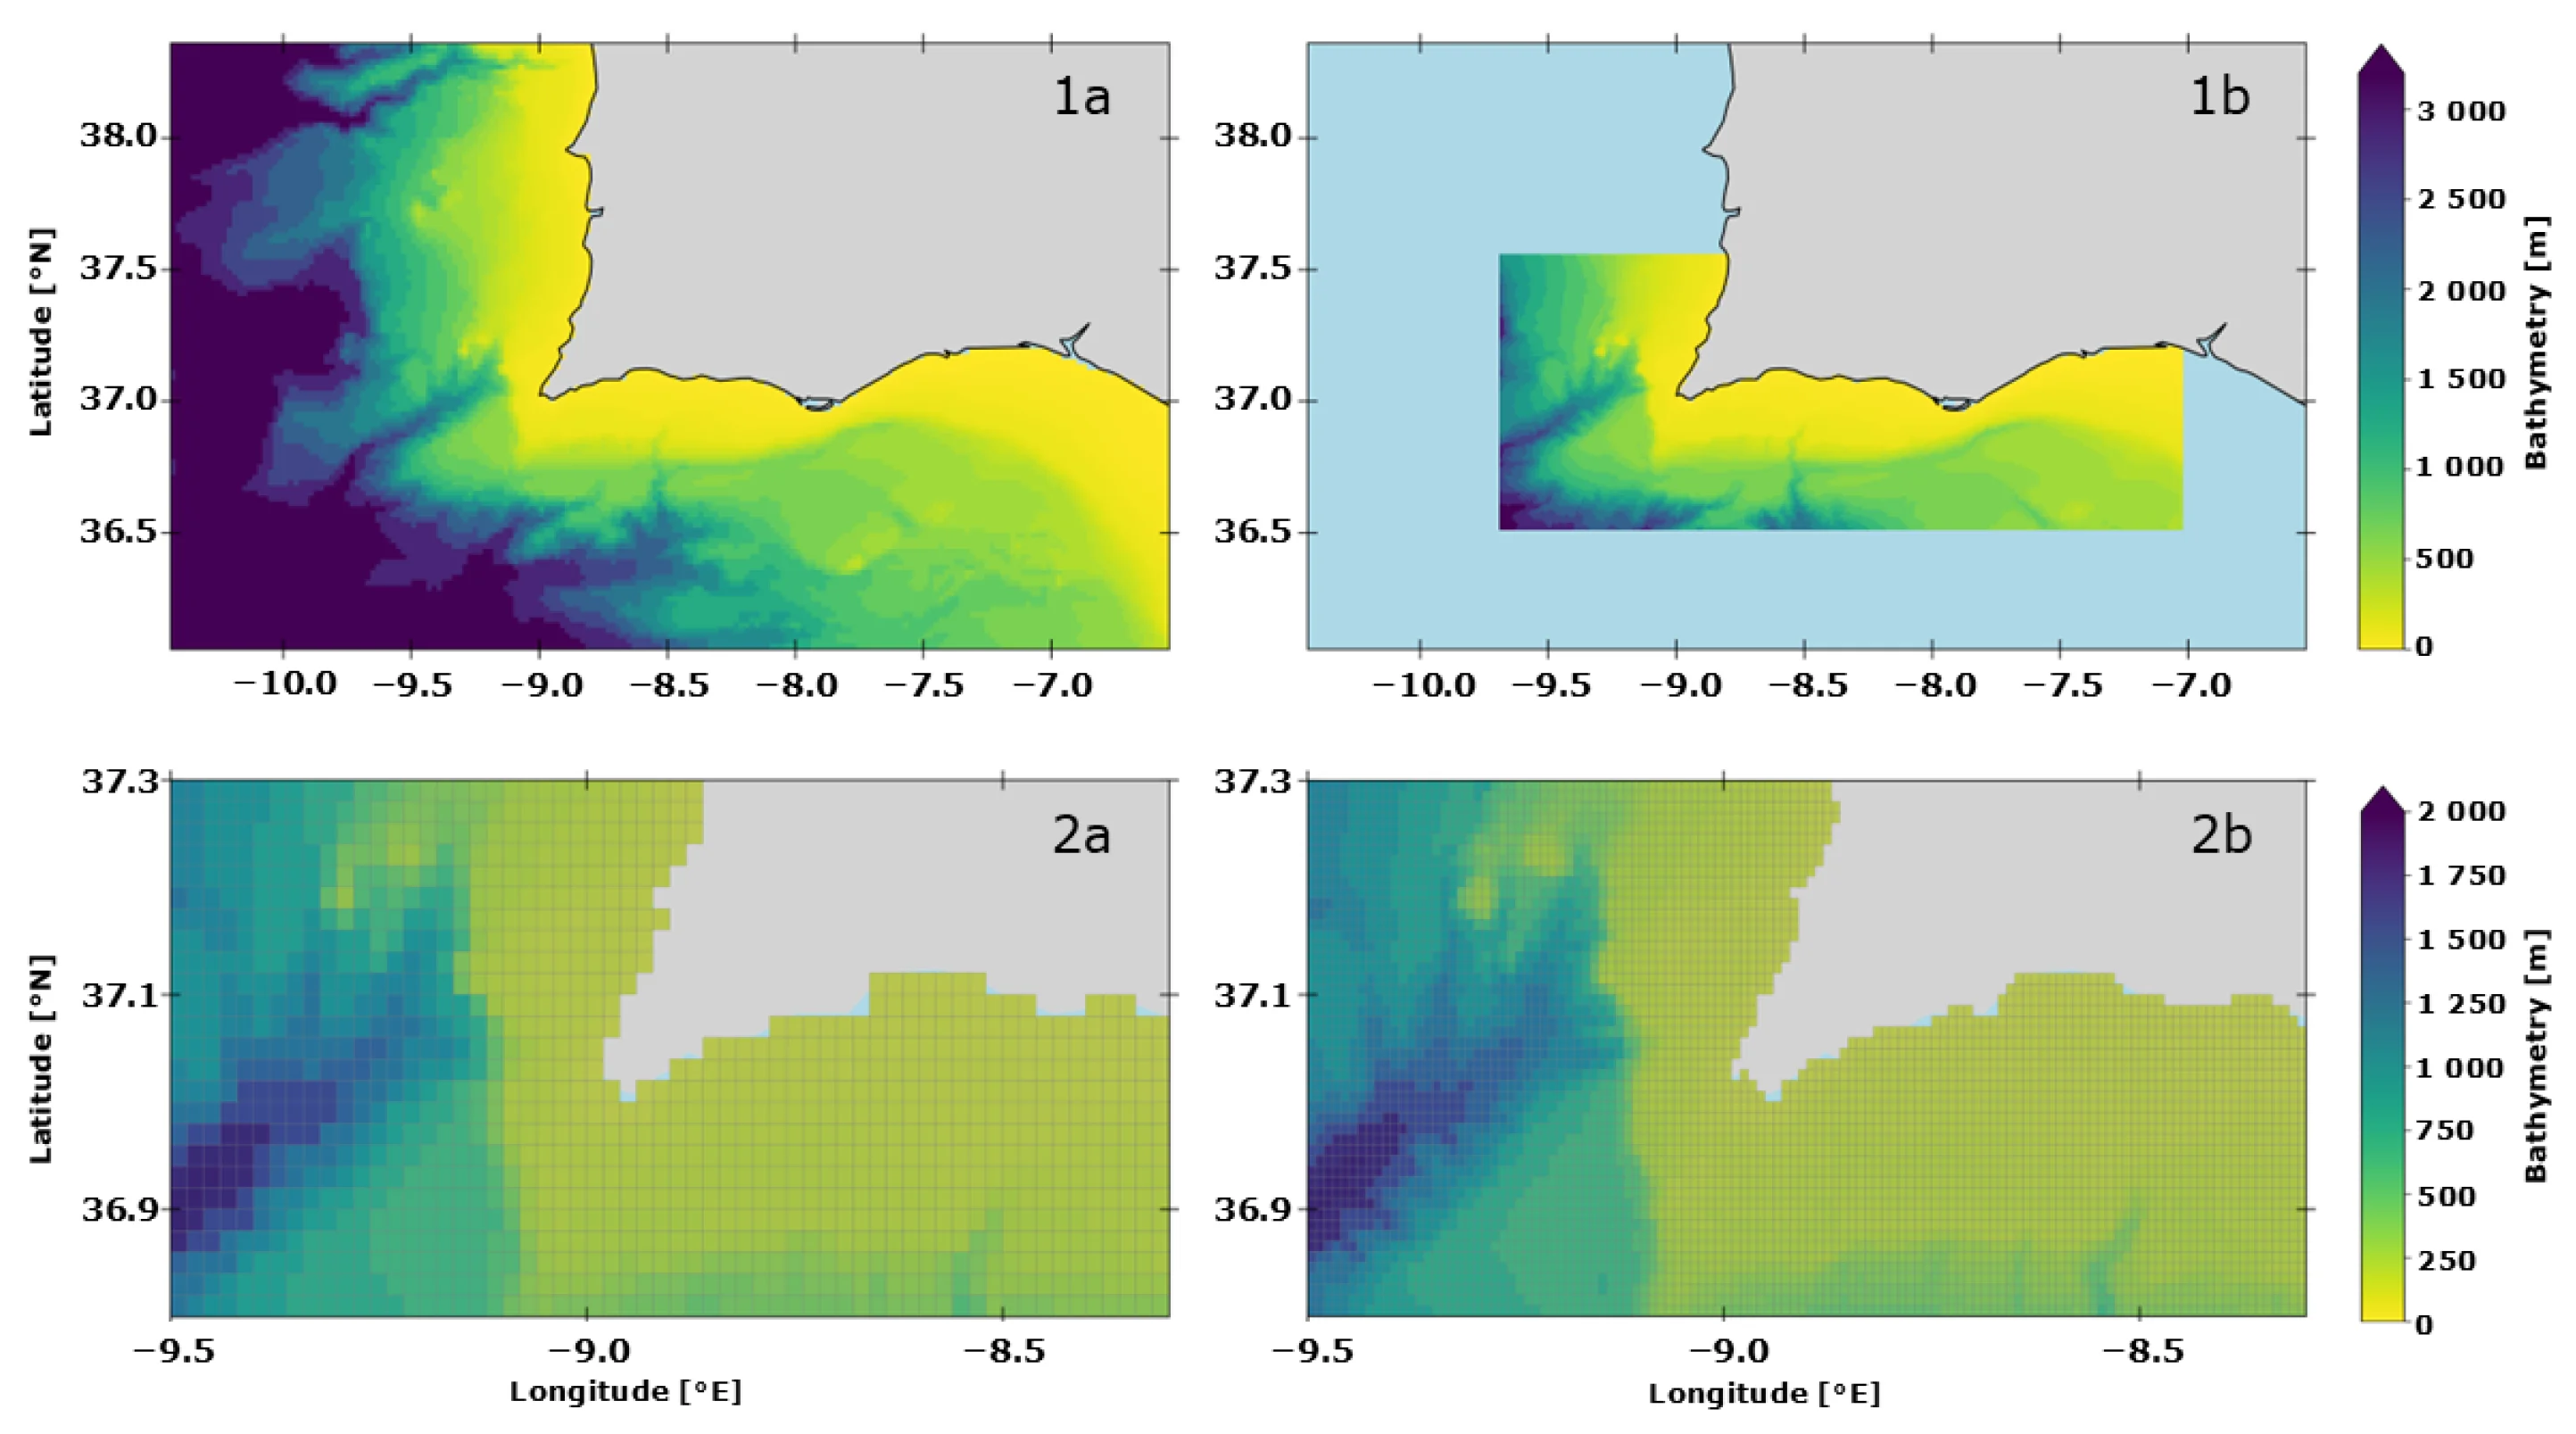
\includegraphics[width=16.0 cm]{figures/fig2.1.png}
    \caption{Spatial domains of the Algarve operational model (SOMA) used in this study. Panels (\textbf{1a}, \textbf{1b}) display the full extent of the SOMA Level 1 and Level 2 grids, respectively. Panels (\textbf{2a}, \textbf{2b}) present a zoomed-in view of the region surrounding Cape St. Vincent, located at the southwestern tip of the Algarve, to highlight the difference in spatial resolution between the two grid levels.}
    \label{fig:batim_2.1}
\end{figure}

In the operational cycle of SOMA, Level 0 is used exclusively to generate tidal boundary conditions and does not produce valid forecast data. In contrast, Levels 1 and 2 provide four-day forecasts of SSH, as well as three-dimensional fields of temperature, salinity, and ocean currents. A noteworthy aspect, as highlighted in \parencite{mendonca2023smscoastal}, is SOMA's operational strategy of performing weekly restart simulations based on CMEMS boundary conditions. This operational configuration serves to update the initial conditions for each new forecast cycle and is explored in the OSSE system implementation for SOMA, as detailed in the following section.

\subsection{SOMA OSSE System Design} \label{subsec:ossedesign_somaosse}
\subsubsection{Nature-Run and Free-Run Configurations}
\hypertarget{subsec:ossedesign_nrfr}{}

As outlined in the objectives of this study, the OSSE system was specifically developed to operate using SOMA as the background model. Given this premise, the ocean-model component of the OSSE is not a variable under investigation but is rather assumed to be a fixed and fully operational system. However, the experiment requires simulation of two different ocean states: one representing the true state (the NR) and another emulating a typical forecast scenario (the FM). In this work, the distinction between NR and FM was achieved by applying the fraternal twins approach, which resulted in using two different configurations of SOMA.

To represent the NR, this study relied on the existing SOMA forecast database for the year 2023. In other words, the key features of the NR within the OSSE system include the use of the Level 2 grid characterized by a horizontal resolution of 1 km and the incorporation of weekly restart cycles based on CMEMS boundary conditions. In contrast, configuring the FM required the introduction of controlled perturbations to SOMA to ensure that its evolution would diverge sufficiently from that of the NR while remaining physically realistic. The FM was initialized with the same initial conditions used for the NR at the start of 2023, as generated by a restart simulation. However, the main structural change involved modifying the Level 2 grid, which was applied over the area illustrated in \bCref{fig:batim_2.1}, panel 1b, by reducing its resolution to 2 km, thereby matching the coarser Level 1 grid shown in panel 2a of the same figure. Furthermore, unlike the NR, the FM was executed continuously throughout 2023 without any weekly updates from CMEMS. As a result, this configuration is referred to as the Free Run (FR), and it constitutes the second instance of SOMA used for comparison against the NR according to the metrics described in Section~\ref{sec:ossedesign_appxA}.

\subsubsection{Data-Assimilation System}
The next fundamental component of the OSSE is the DA system, responsible for incorporating synthetic observations into the FR. The assimilation algorithm employed was based on the formulation presented in \textcite{counillon2023framework}. Modifications were made to ensure compatibility with the SOMA model grid and to enable the reading of synthetic observation data as input, as described in the item \hyperlink{subsec:ossedesign_synthetic}{\textbf{Synthetic Observations and the Reference OSE}} of this Section.

The ensemble used to estimate the background error covariance in the EnOI scheme was sampled from the SOMA FR integration, the same model that was updated by the synthetic observations. Throughout the full-year integration of 2023, model states were extracted at regular intervals, specifically at a rate of one state every 25 h, in order to avoid tidal aliasing; the resulting total comprised 354 ensemble members. This sampling strategy was designed to capture the system's natural variability across the range of oceanographic conditions of the implemented region. Given the strong seasonal behaviour of the Algarve's circulation, as discussed in Section \ref{sec:ossedesign_algarve}, the ensemble was considered sufficient to represent background error structures.

In this implementation, the weighting coefficient $\alpha$, which regulates the balance between the background ensemble variance and the observation error covariance in the analysis update (Section \ref{sec:ossedesign_appxB}), was set to the default value of $1.0$. This choice effectively gives greater weight to the observations. While previous sensitivity studies have shown that smaller values of $\alpha$ may reduce spurious noise at the cost of weaker updates \parencite{counillon2009high}, higher values improve the initial agreement with observations, albeit at the expense of forecast accuracy at longer lead times. Because the present study was dedicated to the development and demonstration of the OSSE framework rather than to parameter optimization, a sensitivity analysis was not performed here. This represents a limitation of the current implementation; therefore, a systematic evaluation of $\alpha$ will be addressed in a future study.

In DA systems, localization functions are commonly employed to reduce the impact of spurious long-range correlations, which are common in ensemble-based DA methods due to finite ensemble size \parencite{carrassi2018data}. Due to this, the localization algorithm implemented in the adopted EnOI scheme was used, considering the Gaspari--Cohn correlation function \parencite{gaspari1999construction}. It is a quasi-Gaussian function that becomes exactly zero beyond a certain distance (compact support) but decreases the correlation values gradually and continuously as the distance increases (smooth tapering). This ensures that the transition from full to zero correlation is smooth, which avoids the introduction of artificial discontinuities into the assimilation process and is effective in addressing the correlation decay issue. The localization radius was set to 10 grid cells, which corresponds to a physical scale of 20 km in the SOMA FR configuration.

\subsubsection{Synthetic Observations and the Reference OSE}
\hypertarget{subsec:ossedesign_synthetic}{}

The final component of the OSSE system is the process of extracting synthetic observations from the NR integration. As previously described, those observations are not actual measurements obtained from external instruments. Instead, they are values picked from a field of SOMA via extraction directly from the model's state vector during the NR simulation. These values are then treated as if they were observational data and assimilated into the FR. To achieve this, a specific procedure was implemented to extract data from the NR outputs at predefined spatial and temporal locations chosen to mimic the structure of a realistic observation network.

Although the assimilation update is applied to the full three-dimensional model domain, the current implementation of the DA system in SOMA was restricted to surface observations. Extending the system to incorporate subsurface data remains a technical challenge due to the complexities of vertical localization and observation operator design. Therefore, it was left for future development. Within this constraint, the experiments employed a univariate DA approach in which SST observations were assimilated to update the complete 3D temperature structure of the model. In other words, temperature was the only variable included in the model state vector of the DA system. This variable has a central role in regulating key oceanic processes such as vertical mixing, stratification, and density-driven circulation. Thus, even when it is assimilated as a single variable, it can exert a wider influence on the modelled ocean state, indirectly improving other variables through the dynamical balances represented in SOMA.

In this context, the synthetic SST observations were extracted from the surface layer of SOMA's Level 2 grid in the NR solution. A hierarchical random strategy based on a spatial sampling approach was implemented. In this approach, the horizontal domain was divided into a regular grid of subareas, each one defined by a fixed number of model grid cells forming a square. Within each subarea, a single observation point was randomly selected using the \verb|randint| function from Python's (version 3.12) \verb|random| module, which generates a pseudo-random integer corresponding to a specific grid cell location. This procedure was applied iteratively across the entire layer, ensuring an irregular but homogeneously distributed set of observations. Consequently, the density of observations depends on the size of the subareas: smaller subareas result in a larger number of observation points, while larger subareas yield fewer but more sparsely distributed observations.

It is crucial to emphasize that for an OSSE system to be reliable, the errors associated with the synthetic observations should not be derived from the NR itself. Instead, they should realistically replicate the kinds of uncertainties present in actual observational systems \parencite{halliwell2014Rigorous}. This requires additional assumptions, as synthetic observations do not originate from physical instruments and thus lack the natural noise introduced by sensors, platforms, or environmental conditions. To guide the estimation of the errors and establish a realistic reference for comparison, two operational satellite-based products covering the SOMA region in 2023 were considered.

\begin{itemize}
	\item CMEMS SST NRT ODYSSEA L4 Product \parencite{eucmems2019ho}: an operational monitoring product providing near-real-time (NRT) SST fields. Updated daily, it is optimized for operational forecasting and rapid environmental monitoring. This product has a finer spatial resolution of $0.02^{\circ}$ and is designed to capture short-term variability. 
	\item CMEMS SST Reprocessed L4 Product \parencite{eucmems2019qa}: a historical, consistently reprocessed climate product that has been available since 1 January 1982. It offers high-quality SST fields produced with rigorous reanalysis methods and quality-control protocols. The product is intended for climate studies and long-term analyses, with a horizontal resolution of $0.05^{\circ}$.   
\end{itemize}

Both satellite products share similar characteristics, providing SST data along with the corresponding estimated observation error standard deviation. Using more than one dataset of the same type ensures that the OSSE system is evaluated under consistent conditions, so that the experiments are expected to produce comparable responses rather than to behave differently depending on the chosen dataset. In addition to their role in defining the OSSE observation errors, these products also served as the observational sources for the reference OSE system. For this purpose, the extraction of data points was restricted to the spatial extent of the NR domain (SOMA Level~2). Within this area, observations were selected using the same pseudo-random sampling strategy previously described for the synthetic data, and for each point, the error value provided by the satellite product was directly applied in the assimilation process of the OSE experiments.

In the OSSE experiments, the procedure to define the observation errors began with identification of the base error value at each observation point from the corresponding satellite product used in the comparative OSE experiment. In other words, if the OSSE configuration was designed to be evaluated against an OSE using the NRT ODYSSEA dataset, then the base error at each synthetic observation point in the OSSE was initially taken from the same spatial location in that product. However, direct assignment of these values would result in an unrealistic equivalence of errors between the systems, contradicting the principle that synthetic observations must emulate, not replicate, real observational noise. To overcome this limitation and preserve the integrity of the OSSE system, a spatially correlated random perturbation field was applied to the base error values. This field was generated using a FORTRAN algorithm based on the methodology described in Appendix E of \parencite{evensen2003ensemble}. The output is a two-dimensional pseudo-random field with horizontal correlation that smoothly varies the values across the model grid to ensure that neighbouring points are not perturbed independently.

Following the exposed methodology, each OSE and OSSE experiment consisted of the assimilation of a single set of surface observations into the FR. The experimental  design involved a structured sequence of steps. First, a set of potential observation points was extracted from the NR grid using the pseudo-random spatial sampling procedure described earlier. From this initial set, a subset was randomly selected, also using the \verb|random| module from Python, to define the number of observations to be assimilated. This reduction process was repeated multiple times using the same base set to generate different observation scenarios containing 10, 50, 100, 200, and 500 data points. Each observation in these sets was associated with an error estimate derived from the corresponding satellite product and perturbed using the spatially correlated random field previously described. Importantly, a different perturbation field was applied to each observation set, ensuring independent spatial patterns of error for each experiment. This behaviour is possible because the FORTRAN program used for generating these fields initializes the random number generator with a seed derived from the system clock, which ensures that a distinct perturbation is produced at each execution over the same model grid. This experimental design is summarized in \bCref{tab:exps_2.1}.

\section{Results and Discussion} \label{sec:ossedesign_results}

This section presents the outcomes of the experiments conducted with the OSSE system configured for the SOMA model. The results are structured into two parts: the first subsection focuses on the analysis of FR integration, which served as the forecast model in the OSSE. It includes a comparison of its temperature fields with the NR, along with an assessment of variability among ensemble members and spatial correlation. The second subsection addresses the core objective of this work: the comparative evaluation of the OSSE and OSE experiments using the various observational scenarios described in the previous section.

\begin{table}[H]
	\centering
	\caption{Summary of the OSE and OSSE experiments. Each experiment is defined by the number of surface observation points assimilated (column \textbf{Number of Points}), the data source from which SST values were extracted (\textbf{Data Source}), and the method used to obtain or estimate the observation errors (\textbf{Observation Error}).}
	\label{tab:exps_2.1}
	\footnotesize
	\begin{tabular}{ccccc}
		\toprule
		\textbf{Experiment}	& \textbf{\shortstack{Number of\\Points}} & \textbf{\shortstack{Data\\Source}} & \multicolumn{2}{c}{\textbf{\shortstack{Observation\\Error}}}\\
		\midrule
		OSE\textsubscript{1} & 10 & \multirow{5}{*}{\shortstack{CMEMS NRT\\ODYSSEA}} & \multicolumn{2}{c}{\multirow{5}{*}{from data source}}\\
		OSE\textsubscript{2} & 50 & & \\
		OSE\textsubscript{3} & 100 & & \\
		OSE\textsubscript{4} & 200 & & \\
		OSE\textsubscript{5} & 500 & & \\
		\midrule
		OSE\textsubscript{6} & 10 & \multirow{5}{*}{\shortstack{CMEMS\\Reprocessed}} & \multicolumn{2}{c}{\multirow{5}{*}{from data source}}\\
		OSE\textsubscript{7} & 50 & & \\
		OSE\textsubscript{8} & 100 & & \\
		OSE\textsubscript{9} & 200 & & \\
		OSE\textsubscript{10} & 500 & & \\
		\midrule
		OSSE\textsubscript{1} & 10 & \multirow{5}{*}{\shortstack{SOMA\\Nature Run}} & \multirow{5}{*}{NRT\_ODYSSEA $\times$} & random\_field\textsubscript{1}\\
		OSSE\textsubscript{2} & 50 & & & random\_field\textsubscript{2}\\
		OSSE\textsubscript{3} & 100 & & & random\_field\textsubscript{3}\\
		OSSE\textsubscript{4} & 200 & & & random\_field\textsubscript{4}\\
		OSSE\textsubscript{5} & 500 & & & random\_field\textsubscript{5}\\
		\midrule
		OSSE\textsubscript{6} & 10 & \multirow{5}{*}{\shortstack{SOMA\\Nature Run}} & \multirow{5}{*}{Reprocessed $\times$} & random\_field\textsubscript{6}\\
		OSSE\textsubscript{7} & 50 & & & random\_field\textsubscript{7}\\
		OSSE\textsubscript{8} & 100 & & & random\_field\textsubscript{8}\\
		OSSE\textsubscript{9} & 200 & & & random\_field\textsubscript{9}\\
		OSSE\textsubscript{10} & 500 & & & random\_field\textsubscript{10}\\
		\bottomrule
	\end{tabular}
\end{table}

\subsection{SOMA Free Run Integration}
The FR simulation was integrated continuously throughout the year 2023, following the configurations and conditions detailed in the item \hyperlink{subsec:ossedesign_nrfr}{\textbf{Nature-Run and Free-Run Configurations}} of Section \ref{subsec:ossedesign_somaosse}. Since SST is the common variable provided by both satellite products selected as observational sources in the reference OSE system, it was also adopted as the basis for assessing the performance of the FR against the NR. Accordingly, the annual evolution of the instantaneous spatial averages (as defined by \bCref{eq:cp2_avg}) and the corresponding RMSEs (\bCref{eq:cp2_rmse}) were computed over the Level~2 domain for both integrations, and the results are presented in the chart in \bCref{fig:sstavg_2.2}.

As shown in \bCref{fig:sstavg_2.2}, the NR and FR exhibit similar seasonal patterns, but their magnitudes vary throughout the year. The RMSE values fluctuate, with higher errors occurring during three distinct periods: early in the year (January-February), in mid-summer (July-August), and late in the year, as the cold season begins. The largest discrepancies align with the transitions between warm and cold seasons, suggesting that the differences between NR and FR are more pronounced during these periods. Despite these differences, the FR solution consistently followed the same seasonal trend as the NR solution did, reflecting a coherent thermal cycle over the year. In certain periods, particularly during spring and early autumn, the SST fields of both solutions were notably close, likely due to the constraint of the shared boundary conditions used in both simulations. Even then, this alignment is seen as a positive result because it reinforces the realism of the FR, while it still represents a degraded solution.

\begin{figure}[H]
	\centering
	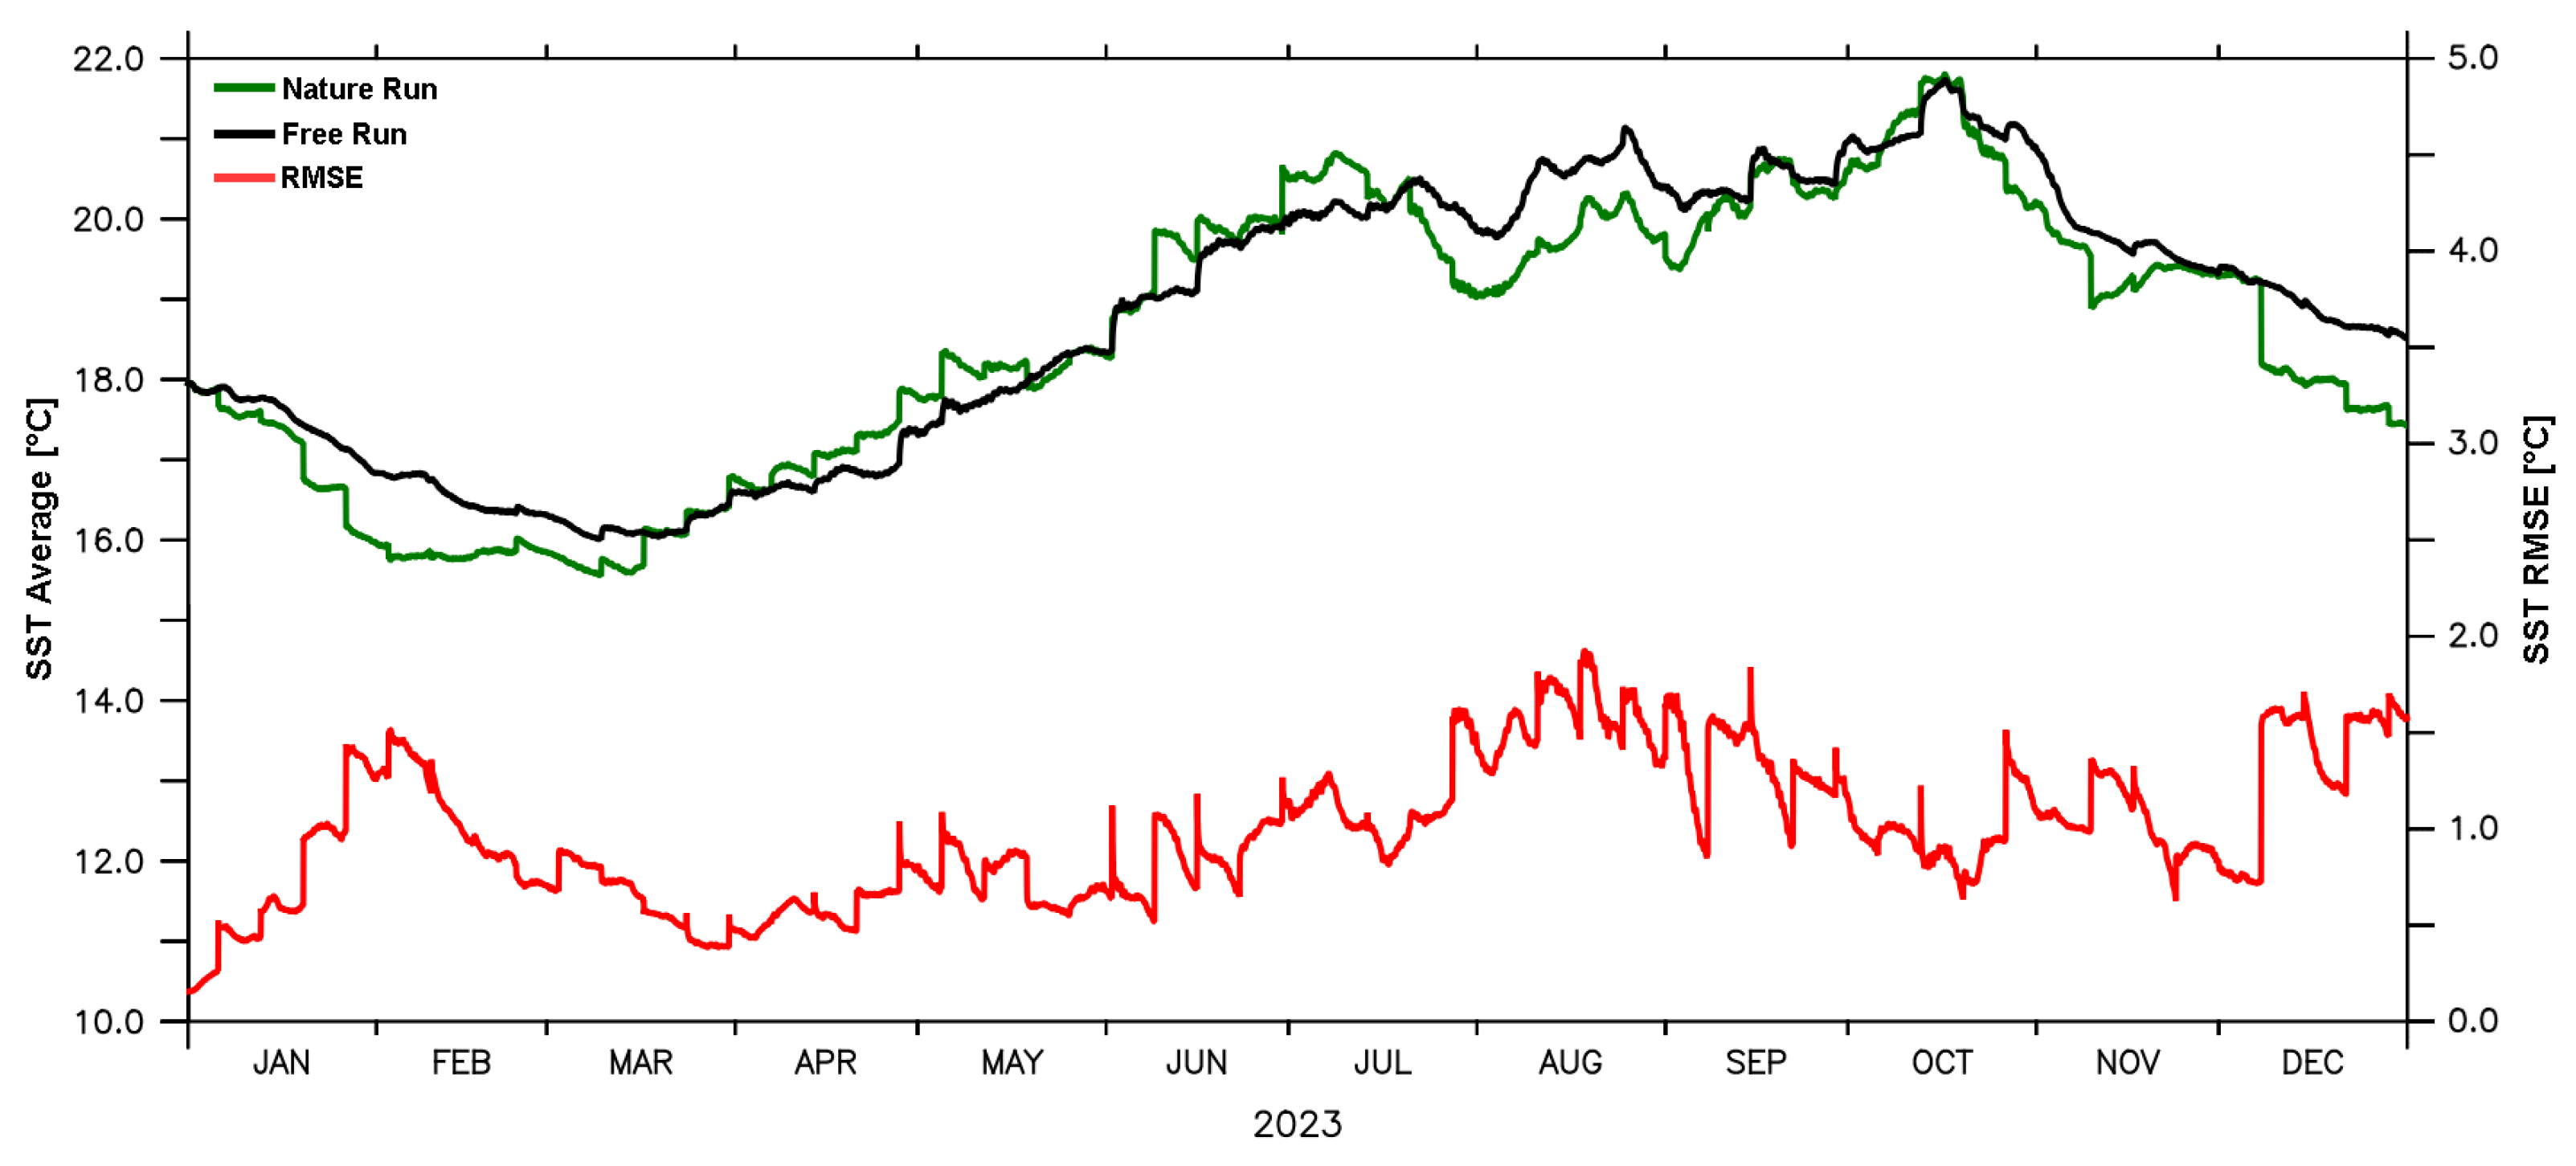
\includegraphics[width=16.0 cm]{figures/fig2.2.png}
	\caption{Comparison of sea surface temperature (SST) between the Nature Run (NR, green line) and the Free Run (FR, black line) over the year 2023. The root mean square error (RMSE) between the temperature fields is shown by the red line, with its scale indicated on the secondary \emph{y}-axis (right)}
	\label{fig:sstavg_2.2}
\end{figure}

A closer inspection of the NR SST curve reveals more pronounced discontinuities, visible as sharp jumps in temperature that are not present in the FR. These abrupt changes are a clear visual indication of the weekly restart simulations implemented in the NR, which force SOMA state variables directly from the updated data of the CMEMS Global solution product. This approach is inherited from the standard SOMA operational forecast framework. Since such updates were deliberately excluded from the FR solution to simulate an unconstrained forecast, these differences further highlight the structural divergence between the two integrations.

It can be inferred that the most significant discrepancies between NR and FR align with the moments of the weekly adjustments, highlighting their influence on the thermal evolution of the NR. This behaviour is particularly evident in the first months of 2023, where the NR solution exhibits a sharper decline in SST compared to the FR in late January and the beginning of February. The influence of the restart mechanism forces the solution to more closely follow the cooling patterns present in the CMEMS data. In contrast, the FR retains more thermal inertia and cools more gradually. At the end of the cold season, the FR lags behind the NR, which begins to recover earlier in response to the updated forcing fields. This example illustrates how the absence of regular external updates in the FR leads to smoother but slower thermal transitions, further supporting the appropriateness of the FR's role as a realistically imperfect forecast scenario within the OSSE framework.

While it is reassuring that the FR solution remained stable and physically consistent, it is nevertheless desirable for it to diverge as much as possible from the NR solution. The larger the discrepancies between them, the greater the system's sensitivity to the observation inputs. This increased sensitivity makes it easier to quantify the added value of the synthetic observations. With this in mind, a specific time frame was selected for conducting both the OSSE and OSE experiments. The selection was guided by the temporal evolution of the RMSE (red curve in \bCref{fig:sstavg_2.2}), which pointed to early February as one of the periods of maximum disagreement between NR and FR. At the same time, it was necessary to consider the availability and quality of satellite observations, which are often affected by cloud cover. Consequently, February 3rd was identified as an optimal date, at it balanced a high RMSE with favourable observational conditions.

Before the observation experiments could begin, an initial assessment of the correlation structure among the ensemble variables in the FR was performed. Given that SST is the primary variable updated through the assimilation process in this system, it was important to examine how it correlates with other physical fields across the model domain. To this end, correlation coefficients were computed between the SST time series at a fixed surface grid cell and the time series of all other variables at each cell within the same horizontal layer. The time series were derived from the FR ensemble members; that is, there was one value for each 25 h period of 2023. Two reference points were selected for this analysis: one located along the southern coast (36.95$^\circ$ N, 7.73$^\circ$ W), an area influenced by the countercurrent system, and another on the western coast (37.29$^\circ$ N, 9.09$^\circ$ W), where coastal upwelling plays a dominant role. The resulting correlation maps, presented in \textbf{Figures}~\bref{fig:corrS_2.3} and~\bref{fig:corrW_2.4}, provide valuable insight into the spatial coherence and dynamical relationships represented by the ensemble.

No correlation plots for SST and SSH are presented here, as the analysis did not reveal any significant relationship between these variables in the FR ensemble. \bCref{fig:corrS_2.3} depicts the correlation maps for the southern reference point. Panels 1.A and 2.A show the correlation between SST and salinity at the surface and at a depth of 100 m, respectively, while panels 1.B and 2.B depict the correlation between SST and horizontal currents at the two same depths. A clear negative correlation is observed between SST and salinity in the ensemble, and this becomes more pronounced with depth. This result indicates that, within the variability represented by the ensemble, colder waters at the surface of the south coast tend to be associated with higher salinity in this region, potentially reflecting the vertical mixing process simulated by the model. In contrast, the correlations between SST and current velocity are weakly positive near the surface and become even less significant at greater depths.

\begin{figure}[H]
	\centering
    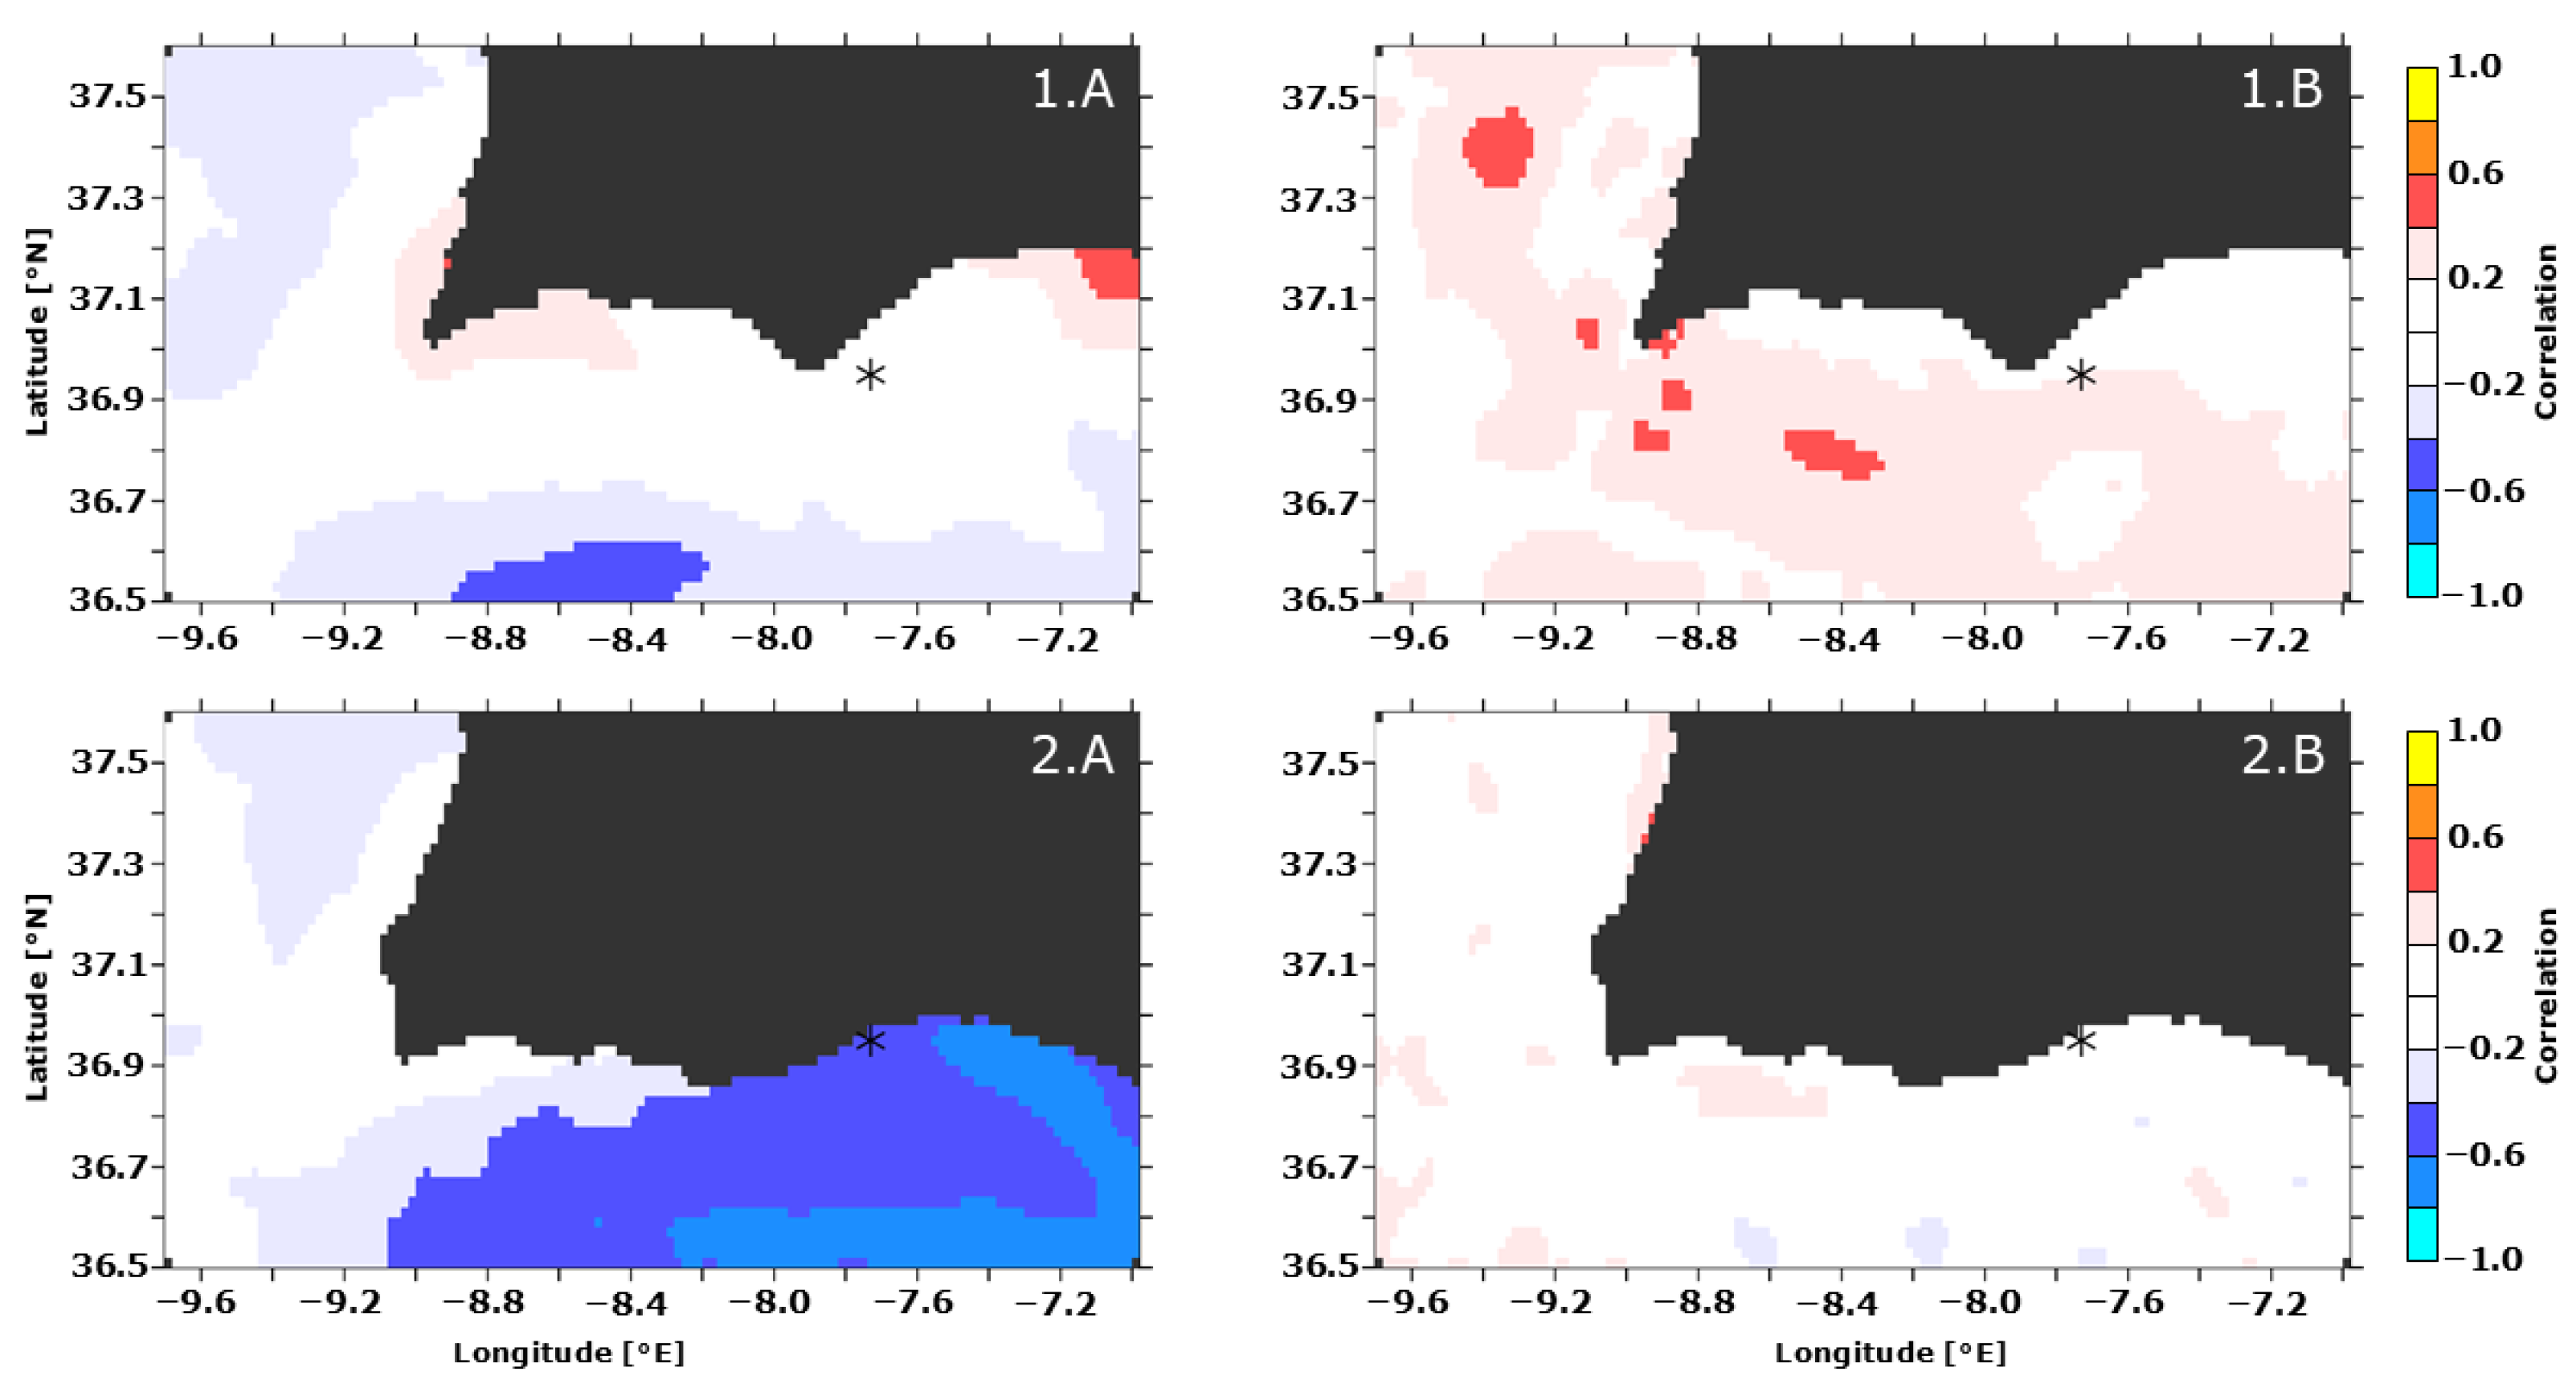
\includegraphics[width=16cm]{figures/fig2.3.png}
    \caption{Correlation maps computed using a reference point on the surface (asterisk on the maps, 36.95$^\circ$ N, 7.73$^\circ$ W). The correlation was calculated over time across all FR ensemble members, relating the surface temperature at this fixed point to salinity and current fields in the rest of the model grid. Maps (\textbf{1.A},\textbf{1.B}) show the correlations at the surface for salinity and currents, respectively. Maps~(\textbf{2.A},\textbf{2.B}) depict the same properties at a depth of 100 m.}
    \label{fig:corrS_2.3}
\end{figure}

\begin{figure}[H]
	\centering
	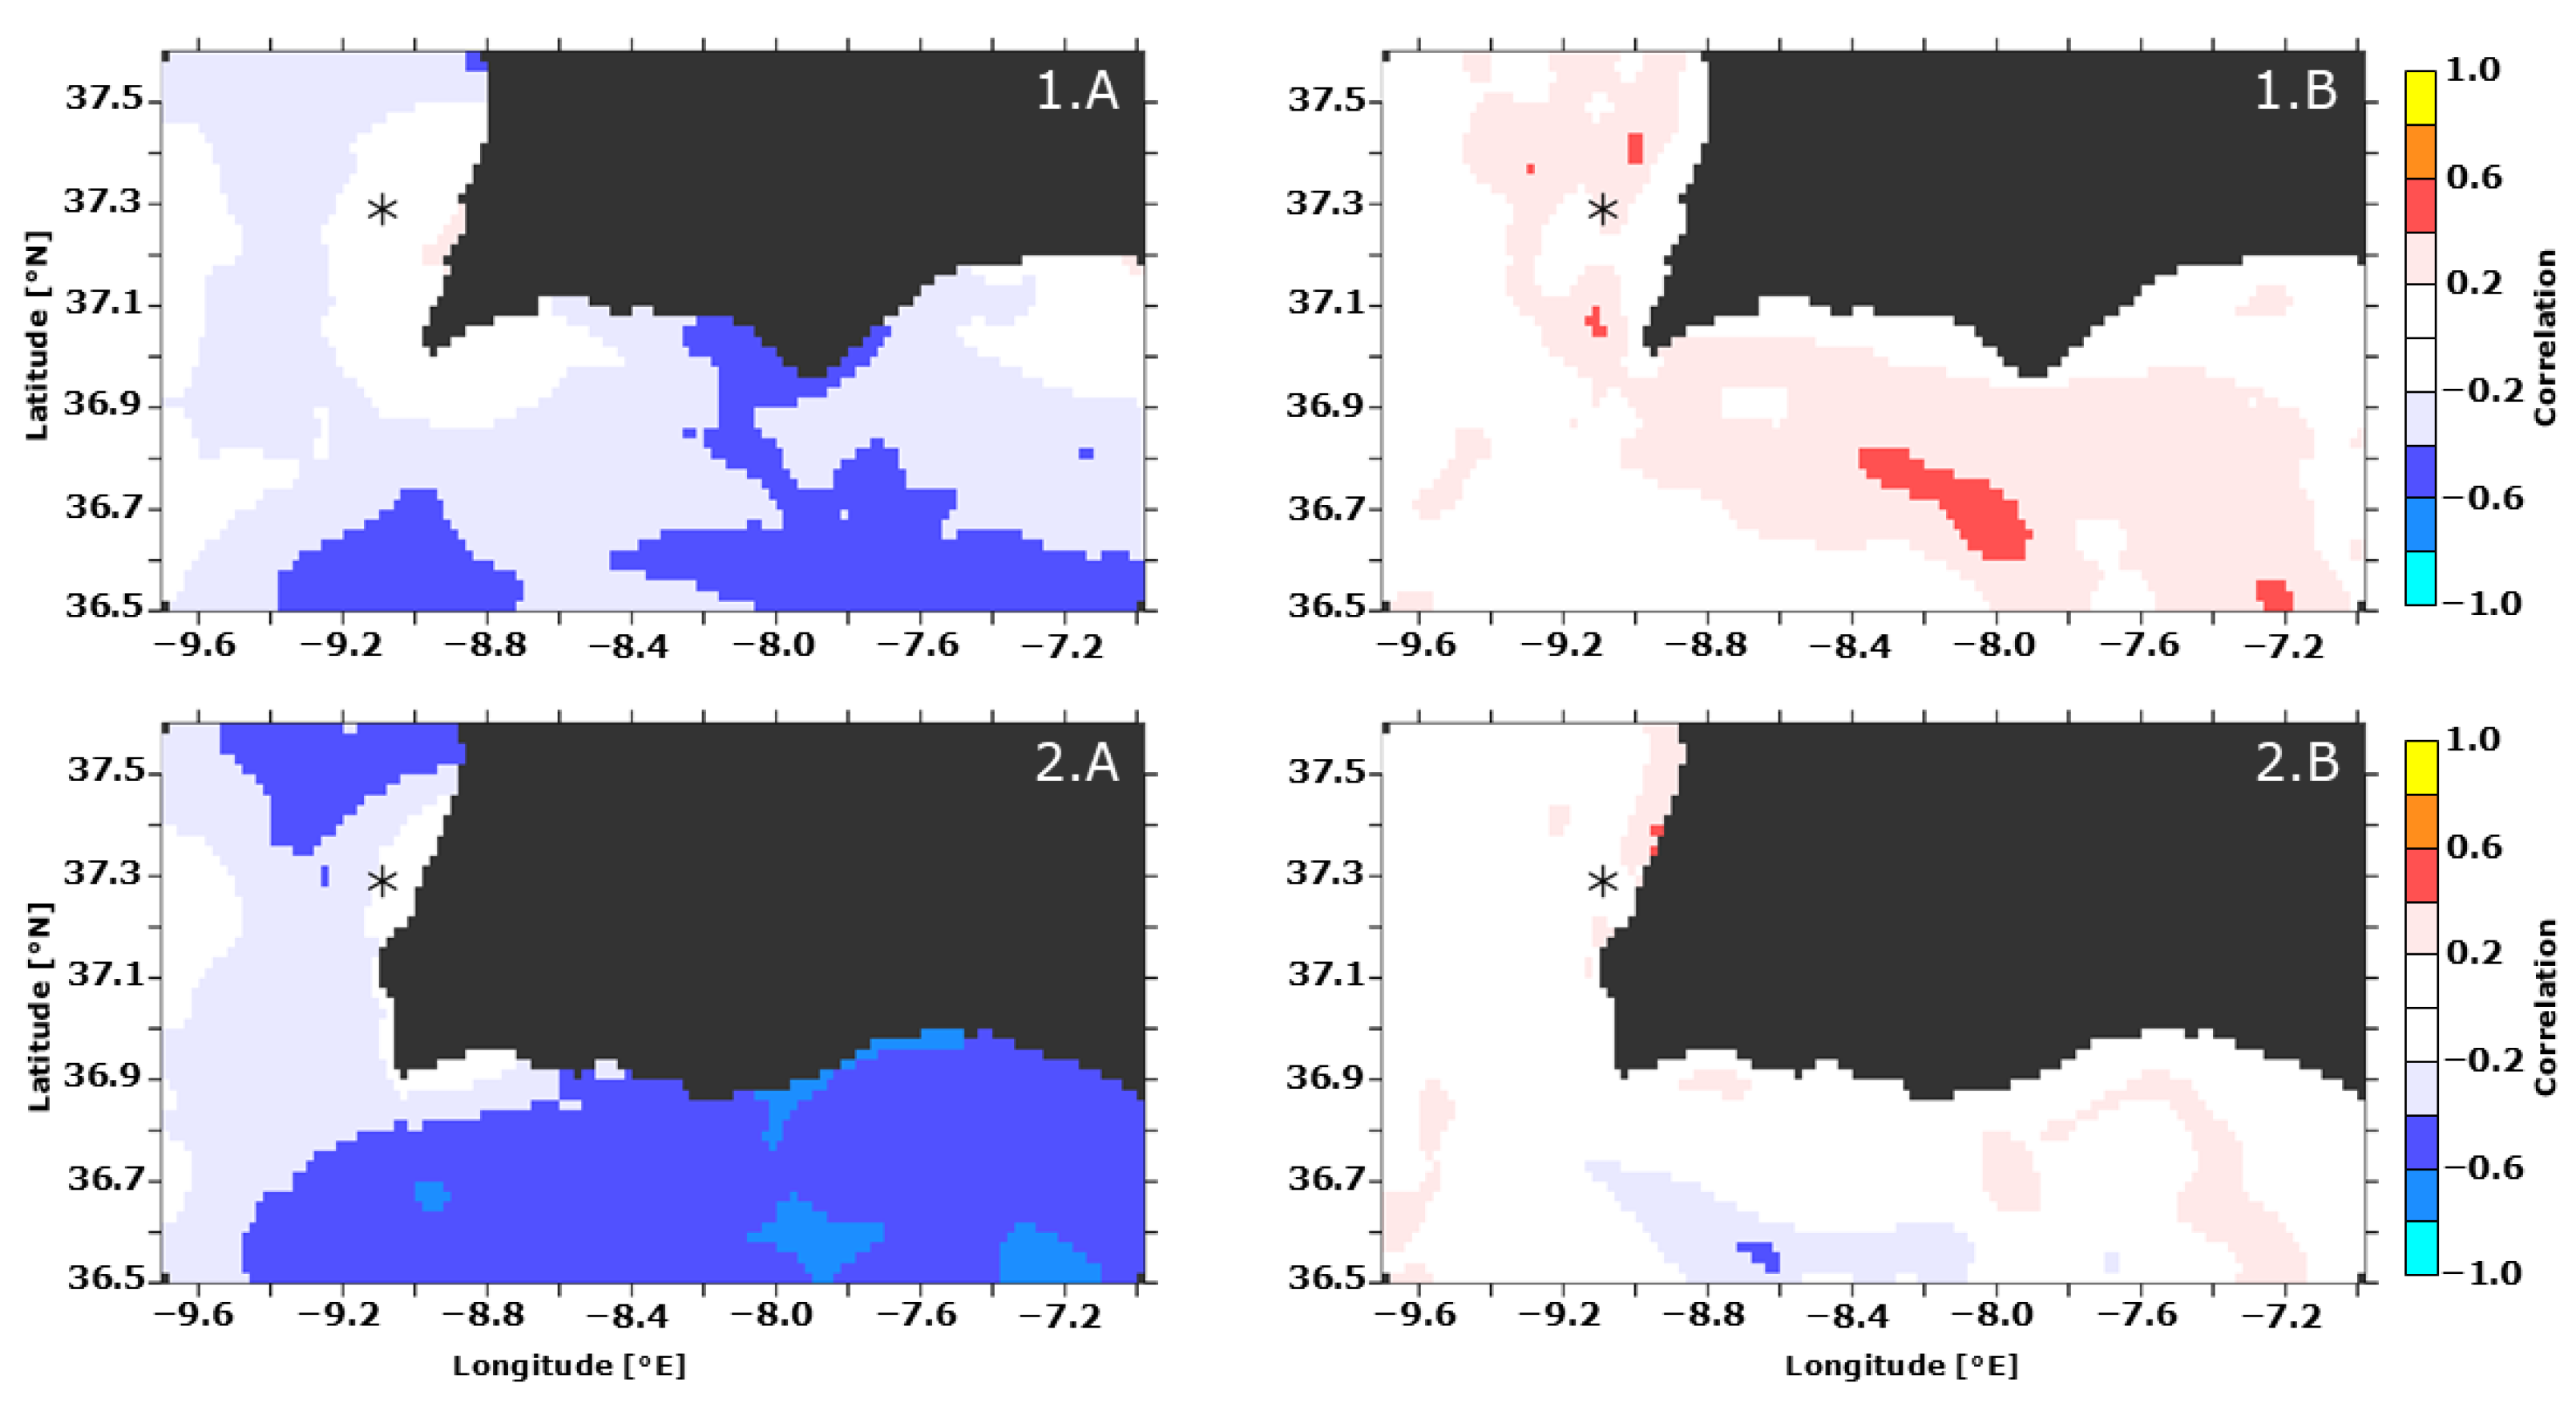
\includegraphics[width=16cm]{figures/fig2.4.png}
	\caption{Correlation maps computed using a reference point on the surface (asterisk on the maps, 37.29$^\circ$ N, 9.09$^\circ$ W) on the western coast of the domain. The correlation was calculated over time across all FR ensemble members, relating the surface temperature at this fixed point to salinity and current fields in the rest of the model grid, following the same methodology as in \bCref{fig:corrS_2.3}. Maps (\textbf{1.A},\textbf{1.B}) show the correlation at the surface for salinity and currents, respectively, while Maps (\textbf{2.A},\textbf{2.B}) depict the same properties at a depth of 100 m.}
	\label{fig:corrW_2.4}
\end{figure}

\newpage
A similar pattern is observed in the maps shown in \bCref{fig:corrW_2.4}, which correspond to the western reference point influenced by upwelling. Again, panels 1.A and 2.A show the correlation with salinity at the surface and 100 m, while 1.B and 2.B refer to the correlation with horizontal currents. As in the southern region, SST is negatively correlated with salinity in the ensemble, and this correlation intensifies with depth. The relationship with currents shows a limited positive correlation near the surface that diminishes with depth, indicating that there is only a modest association between thermal variability and current patterns within the ensemble in this area as well.

Given the consistent negative correlation patterns between SST and salinity observed in \textbf{Figures}~\bref{fig:corrS_2.3} and~\bref{fig:corrW_2.4}, a vertical profile analysis was conducted to further investigate this relationship throughout the water column. Using the same two reference locations, the correlation  between the surface SST and salinity values was computed at increasing depths at each respective point. Hence, for each spot, the correlation was computed over time across all ensemble members and repeated for all vertical salinity levels in the model. The results (\bCref{fig:corrz_2.5}) reveal a clear intensification of the negative correlation with depth. The red curve represents the profile for the southern coast reference point, while the blue curve corresponds to the western location. In both cases, the strength of the inverse relationship increases steadily with distance below the surface, confirming that the inverse relationship between temperature and salinity becomes more pronounced with depth in the ensemble.

The results presented in \textbf{Figures}~\bref{fig:corrS_2.3}--\bref{fig:corrz_2.5} suggest a negative correlation between SST and salinity within the FR ensemble that becomes particularly pronounced at greater depths. Given that the OSSE system is based on an EnOI data-assimilation scheme, such a statistical relationship could, in principle, be leveraged in a multivariate assimilation framework \parencite{counillon2009ensemble, turner2005assimilation}. This would allow SST observations to contribute indirectly to salinity updates, potentially improving the model's representation of water mass properties and thermohaline structure. Such an approach also carries practical implications for the design of observing systems, as exploiting multivariate updates from SST could lessen the reliance on dedicated salinity measurements and thereby enable the deployment of lower-cost observing technologies and more extensive large-scale monitoring networks.

Although the ensemble reveals a statistical relationship between SST and salinity, the physical basis of this negative correlation remains uncertain. Specifically, in the southern region of the domain, a positive correlation between SST and salinity was initially anticipated, considering the influence of easterly winds that occur offshore of the south coast. These winds transport warm, saline Mediterranean waters toward the Algarve shelf and often alternate with westerly winds along the coastline (Section~\ref{sec:ossedesign_algarve}). The dynamics of these alternating wind regimes and their impact on surface and subsurface water properties may not be fully captured by the FR ensemble, especially if its sampling fails to represent the full range of seasonal variability. For this reason, and to preserve methodological clarity, the current implementation of the OSSE system was limited to temperature updates only, leaving multivariate approaches for future development once the underlying mechanisms are better understood.

\begin{figure}[H]
	\centering
	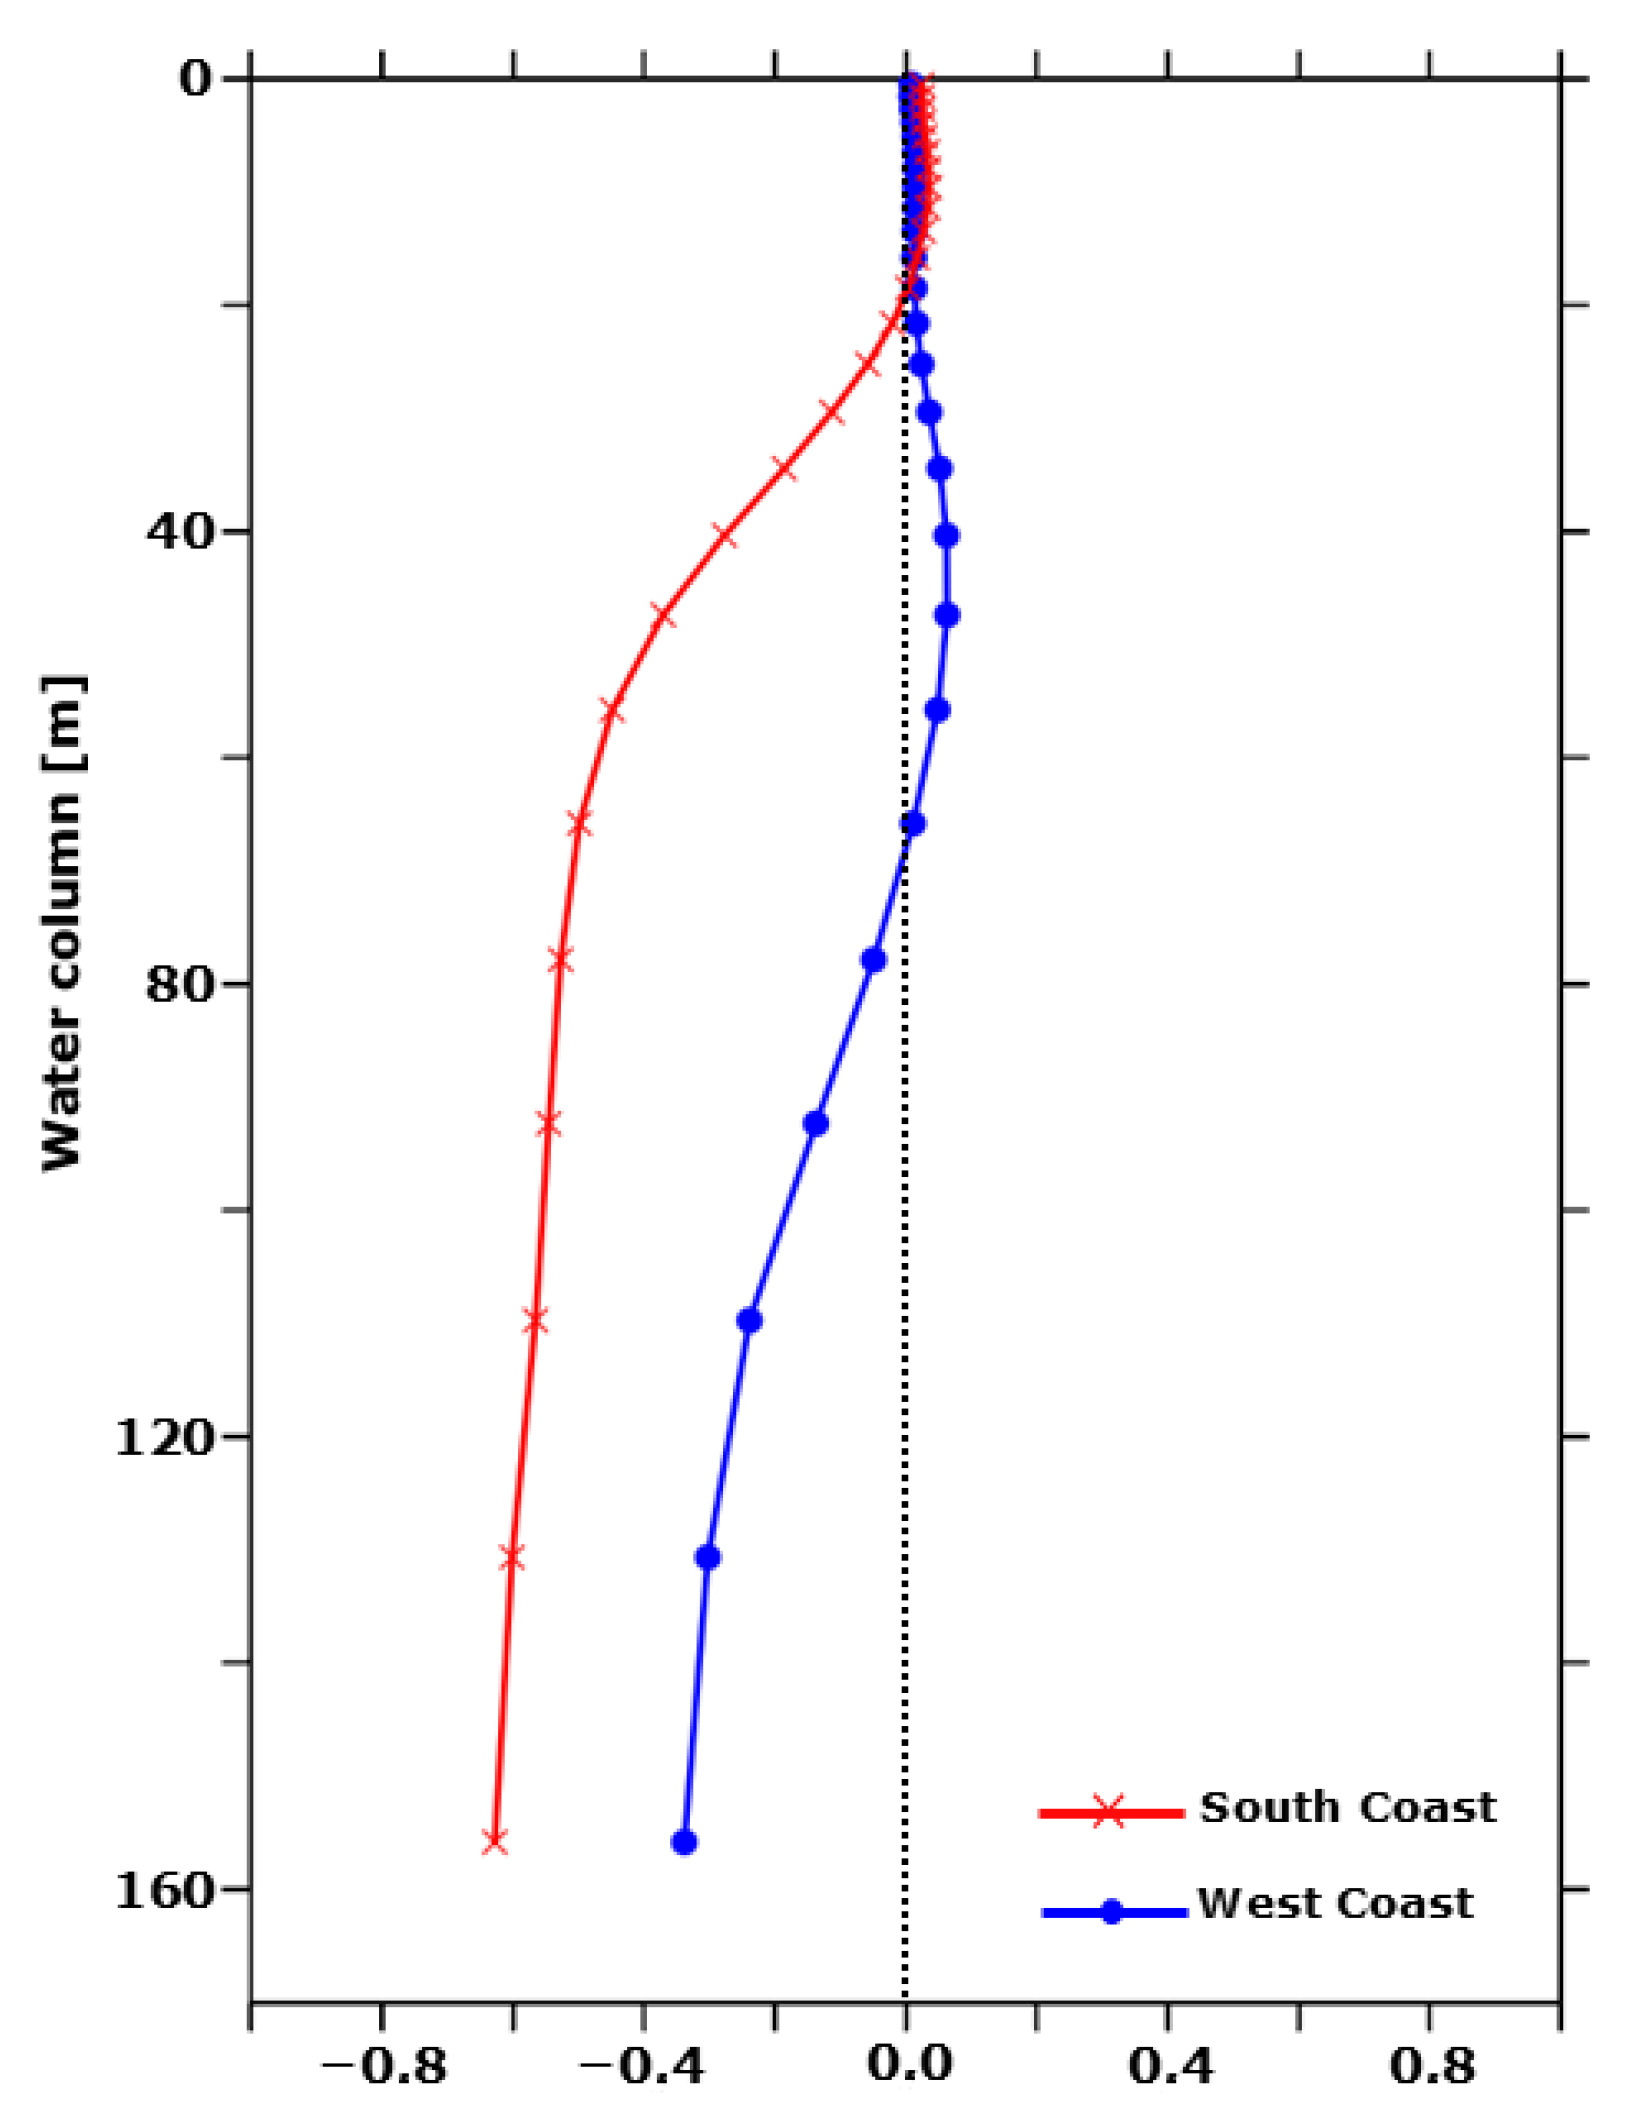
\includegraphics[width=9.0cm]{figures/fig2.5.png}
	\caption{Depth-dependent correlation between SST and salinity over time, calculated using the FR ensemble members. Each curve corresponds to a reference location within the model domain: the southern coast of Portugal (36.95$^\circ$ N, 7.73$^\circ$ W; red curve, same as \bCref{fig:corrS_2.3}) and the western coast (37.29$^\circ$ N, 9.09$^\circ$ W; blue curve, same as \bCref{fig:corrW_2.4}).}
	\label{fig:corrz_2.5}
\end{figure}

\subsection{SOMA OSSE System Assessment}

The performance and internal structure of the FR having been established, this section presents how it responded to the updates derived from the synthetic observations generated in the NR, as well as a comparative evaluation of the OSSE experiments and their corresponding OSE configurations. These analyses aimed to quantify the behaviour of the OSSE system to ensure that, when applied to assess new observation strategies, it would not systematically overestimate or underestimate their value.

Regarding the pseudo-random perturbation fields introduced in the item \hyperlink{subsec:ossedesign_synthetic}{\textbf{Synthetic Observations and the Reference OSE}} of \Cref{subsec:ossedesign_somaosse}, a horizontal decorrelation length had to be defined to determine the spatial scale over which values in a generated field remained correlated. This distance reflected the approximate range at which SST values in the L3 satellite products appear spatially coherent prior to their processing into the corresponding L4 gridded datasets. For this reason, a value of 25~km was selected, corresponding to 25 cells in the 1 km NR grid.

Knowing that 3 February 2023 was selected as the date for the updates, each experiment was subsequently integrated for an additional seven days to evaluate the temporal evolution of the forecast after the assimilation step. \bCref{fig:rmsenrt_2.6} presents the results of this post-assimilation period for the experiments based on the NRT ODYSSEA product. In the left-hand panel, the daily evolution of the SST RMSE is shown for each OSE experiment relative to the satellite observations, with the black curve representing the baseline FR error. The remaining curves correspond to OSEs using an increasing number of assimilated observation points, from 10 in OSE1 to 500 in OSE5, as listed in \bCref{tab:exps_2.1}. The right-hand panel displays the corresponding SST RMSE for the OSSE experiments, which assimilated synthetic observations and were evaluated against the NR. As expected, experiments using the Reprocessed product exhibited behaviour very similar to the behaviour of those that used the NRT ODYSSEA data. Therefore, the RMSE results from the Reprocessed-based experiments are presented in \Cref{sec:cp2_supp}


\begin{figure}[H]
    \centering
    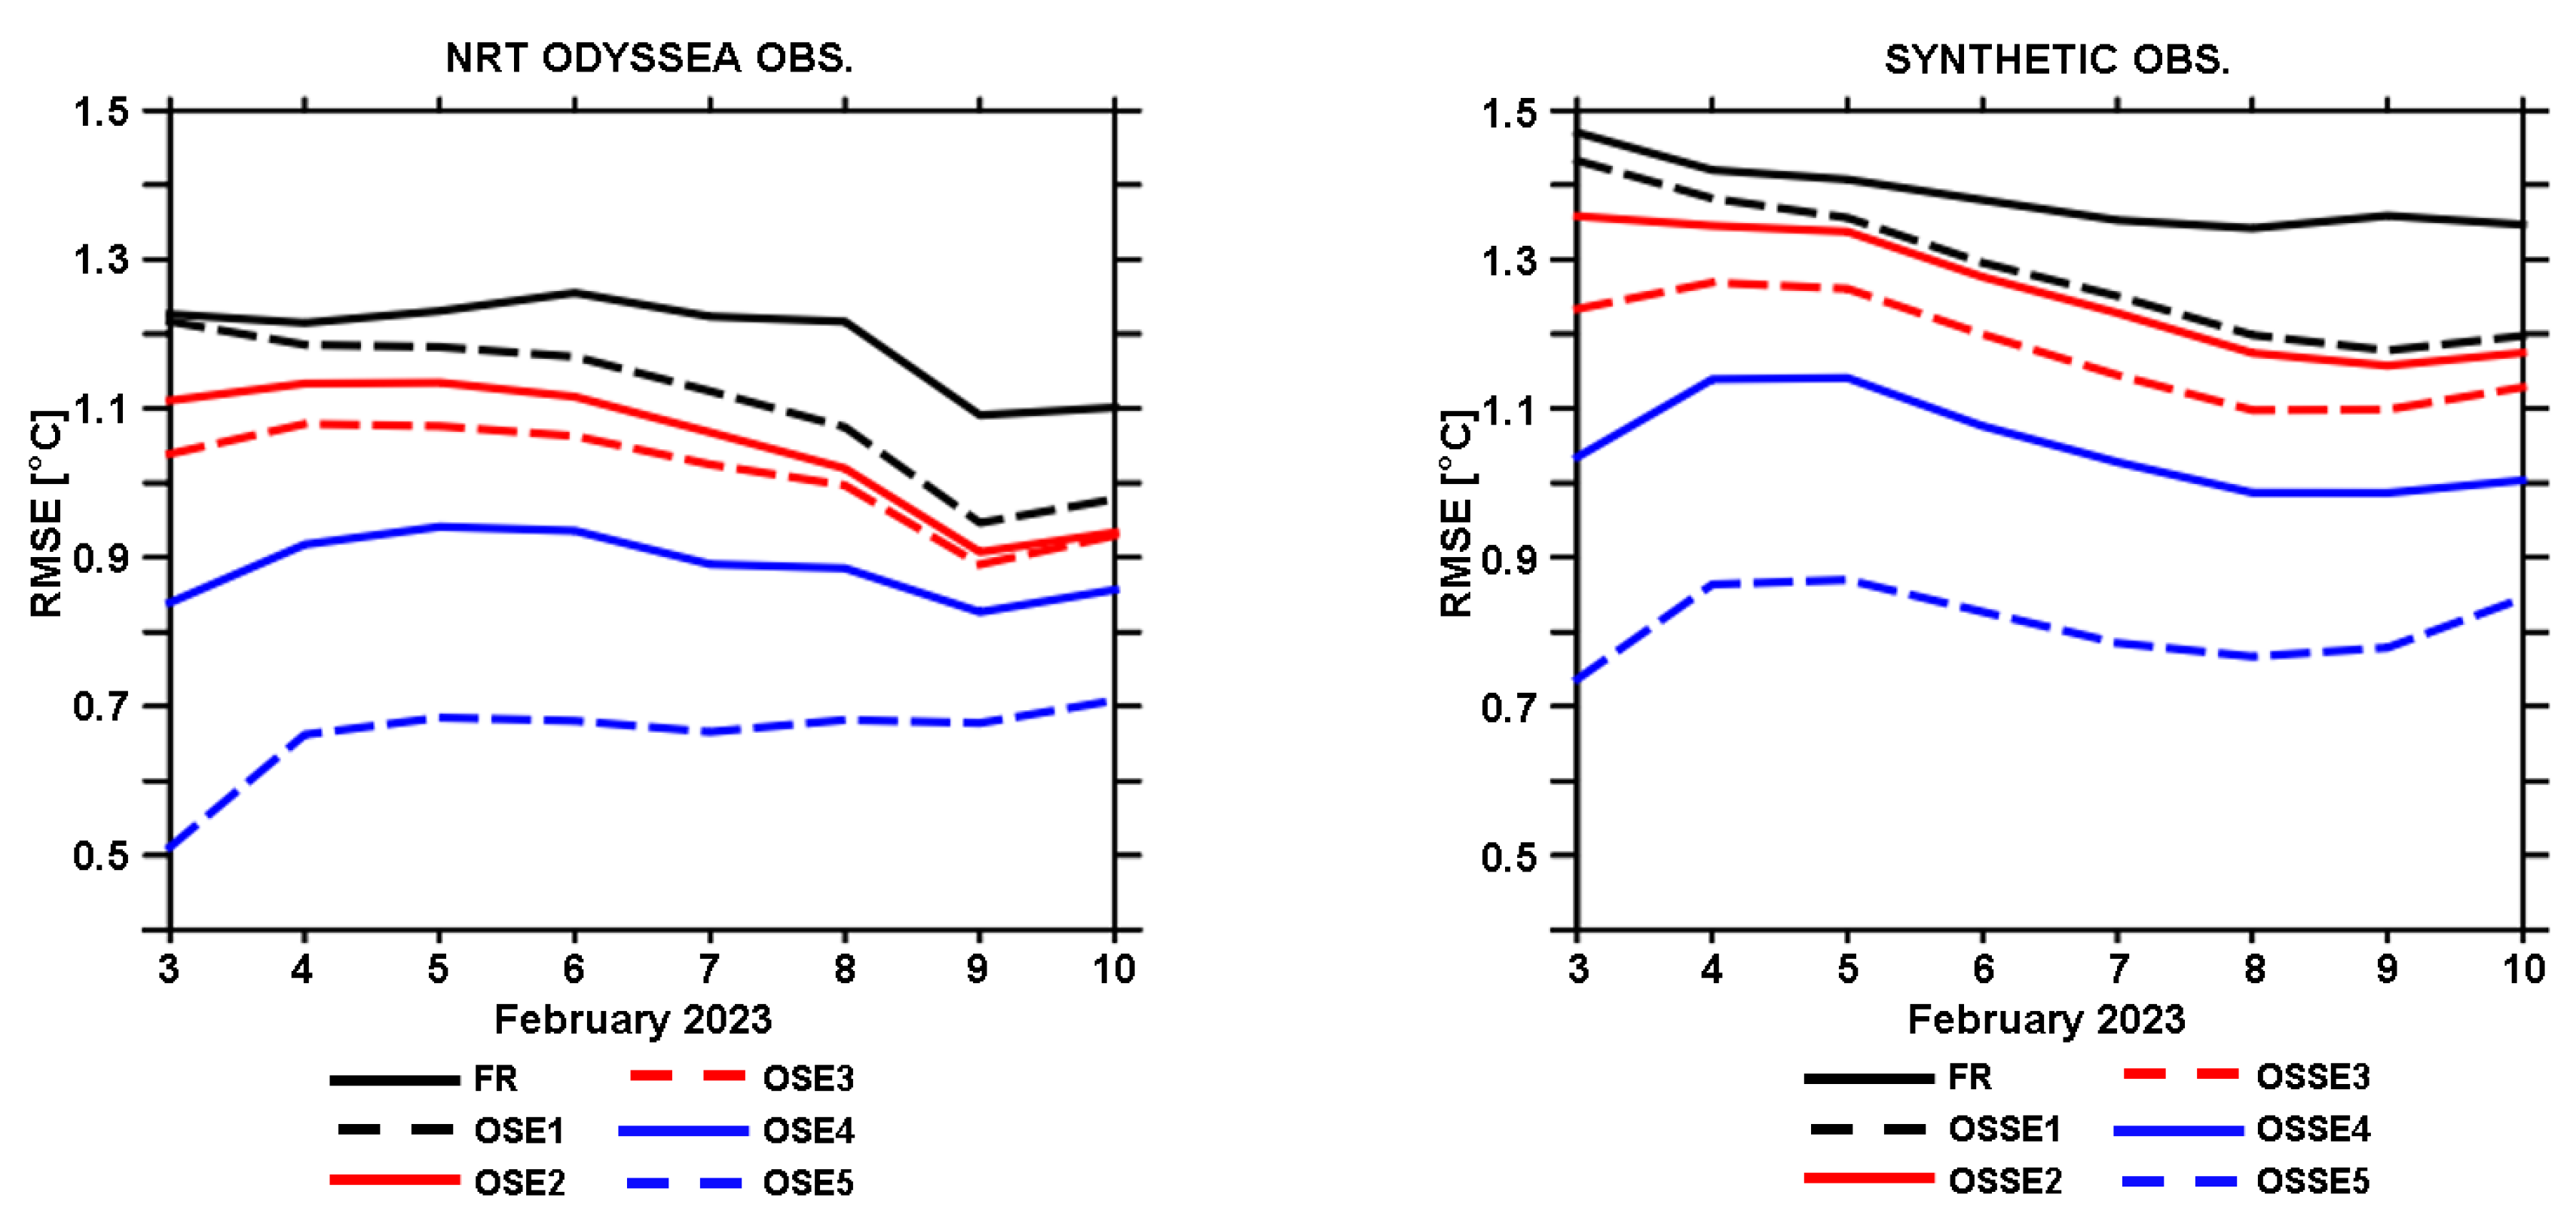
\includegraphics[width=15.0cm]{figures/fig2.6.png}
    \caption{On the left, the SST error over time of the FR and experiments OSE1 to OSE5, referenced in \bCref{tab:exps_2.1}, with respect to the NRT ODYSSEA satellite product. On the right, the SST error of the FR and experiments OSSE1 to OSSE5 with respect to the NR. The experiments were integrated for an additional seven days following the update on 3 February.}
    \label{fig:rmsenrt_2.6}
\end{figure}

A detailed analysis of \bCref{fig:rmsenrt_2.6} provides important insights into the OSSE system's behaviour following the updates. Most likely due to the random multiplicative factor that increases the observation errors, the RMSE of the FR with respect to the NR is consistently higher than the RMSE relative to the satellite observations. However, the emphasis here is not on this absolute difference, but on the relative consistency across experiments. Both OSE and OSSE configurations exhibit a clear, monotonic reduction in RMSE as the number of assimilated observations increases. The temporal evolution also shows that, as expected, assimilating a large number of observations produces a gradual increase in RMSE in the days following the update, whereas assimilating only a few points tends to increase the RMSE at analysis time, with the resulting dynamical inconsistencies causing more harm than benefit.

Notably, the OSSE experiments closely mirror the behaviours of their corresponding OSE counterparts over time, despite relying solely on synthetic data. For each observation count, the RMSE curves of the OSSEs follow trends that are closely aligned with those of the OSEs, indicating that the synthetic updates generate corrections in the model state that are dynamically comparable to those achieved through the assimilation of real satellite observations. This agreement is particularly clear when comparing experiments configured with the same number of assimilated observations (e.g., OSE3 versus OSSE3). Comparable consistency was also found when repeating the experiments with the Reprocessed satellite product, reinforcing that the OSSE system responds similarly when assimilating equivalent datasets. Had the results from the Reprocessed product diverged substantially from those using the NRT ODYSSEA data, it could have indicated shortcomings in the system's design and the need for further refinement.

In addition to the temporal RMSE analysis, Taylor diagrams were used to evaluate the similarity between the forecast fields and the reference data. These were generated for two instants: the day of the EnOI update step (3 February) and seven days afterward (10 February). \bCref{fig:taylornrt_2.7} presents the results for the experiments based on the NRT ODYSSEA satellite product. In line with previous RMSE-based assessment, the overall patterns in the diagrams are consistent. The most relevant aspect lies not in the precise values, but in the comparative behaviour of OSSEs relative to OSEs. The satellite data (SAT\_NRT in the figure) and the NR serve as reference anchors, with SAT\_NRT exhibiting a higher standard deviation, reflecting its origin as a gridded observational product. As observations are progressively assimilated into the FR, the forecast state converges toward the reference: the OSE experiments (red markers) move closer to SAT\_NRT, while the OSSE experiments (yellow markers) approach the NR. Although the OSSEs show slightly higher root mean square differences (RMSD) than the OSEs, consistent with the RMSE trends, both follow remarkably similar trajectories in terms of correlation and RMSD reduction. This convergence was also evident in the experiments using the Reprocessed satellite product.

\begin{figure}[H]
    \centering
    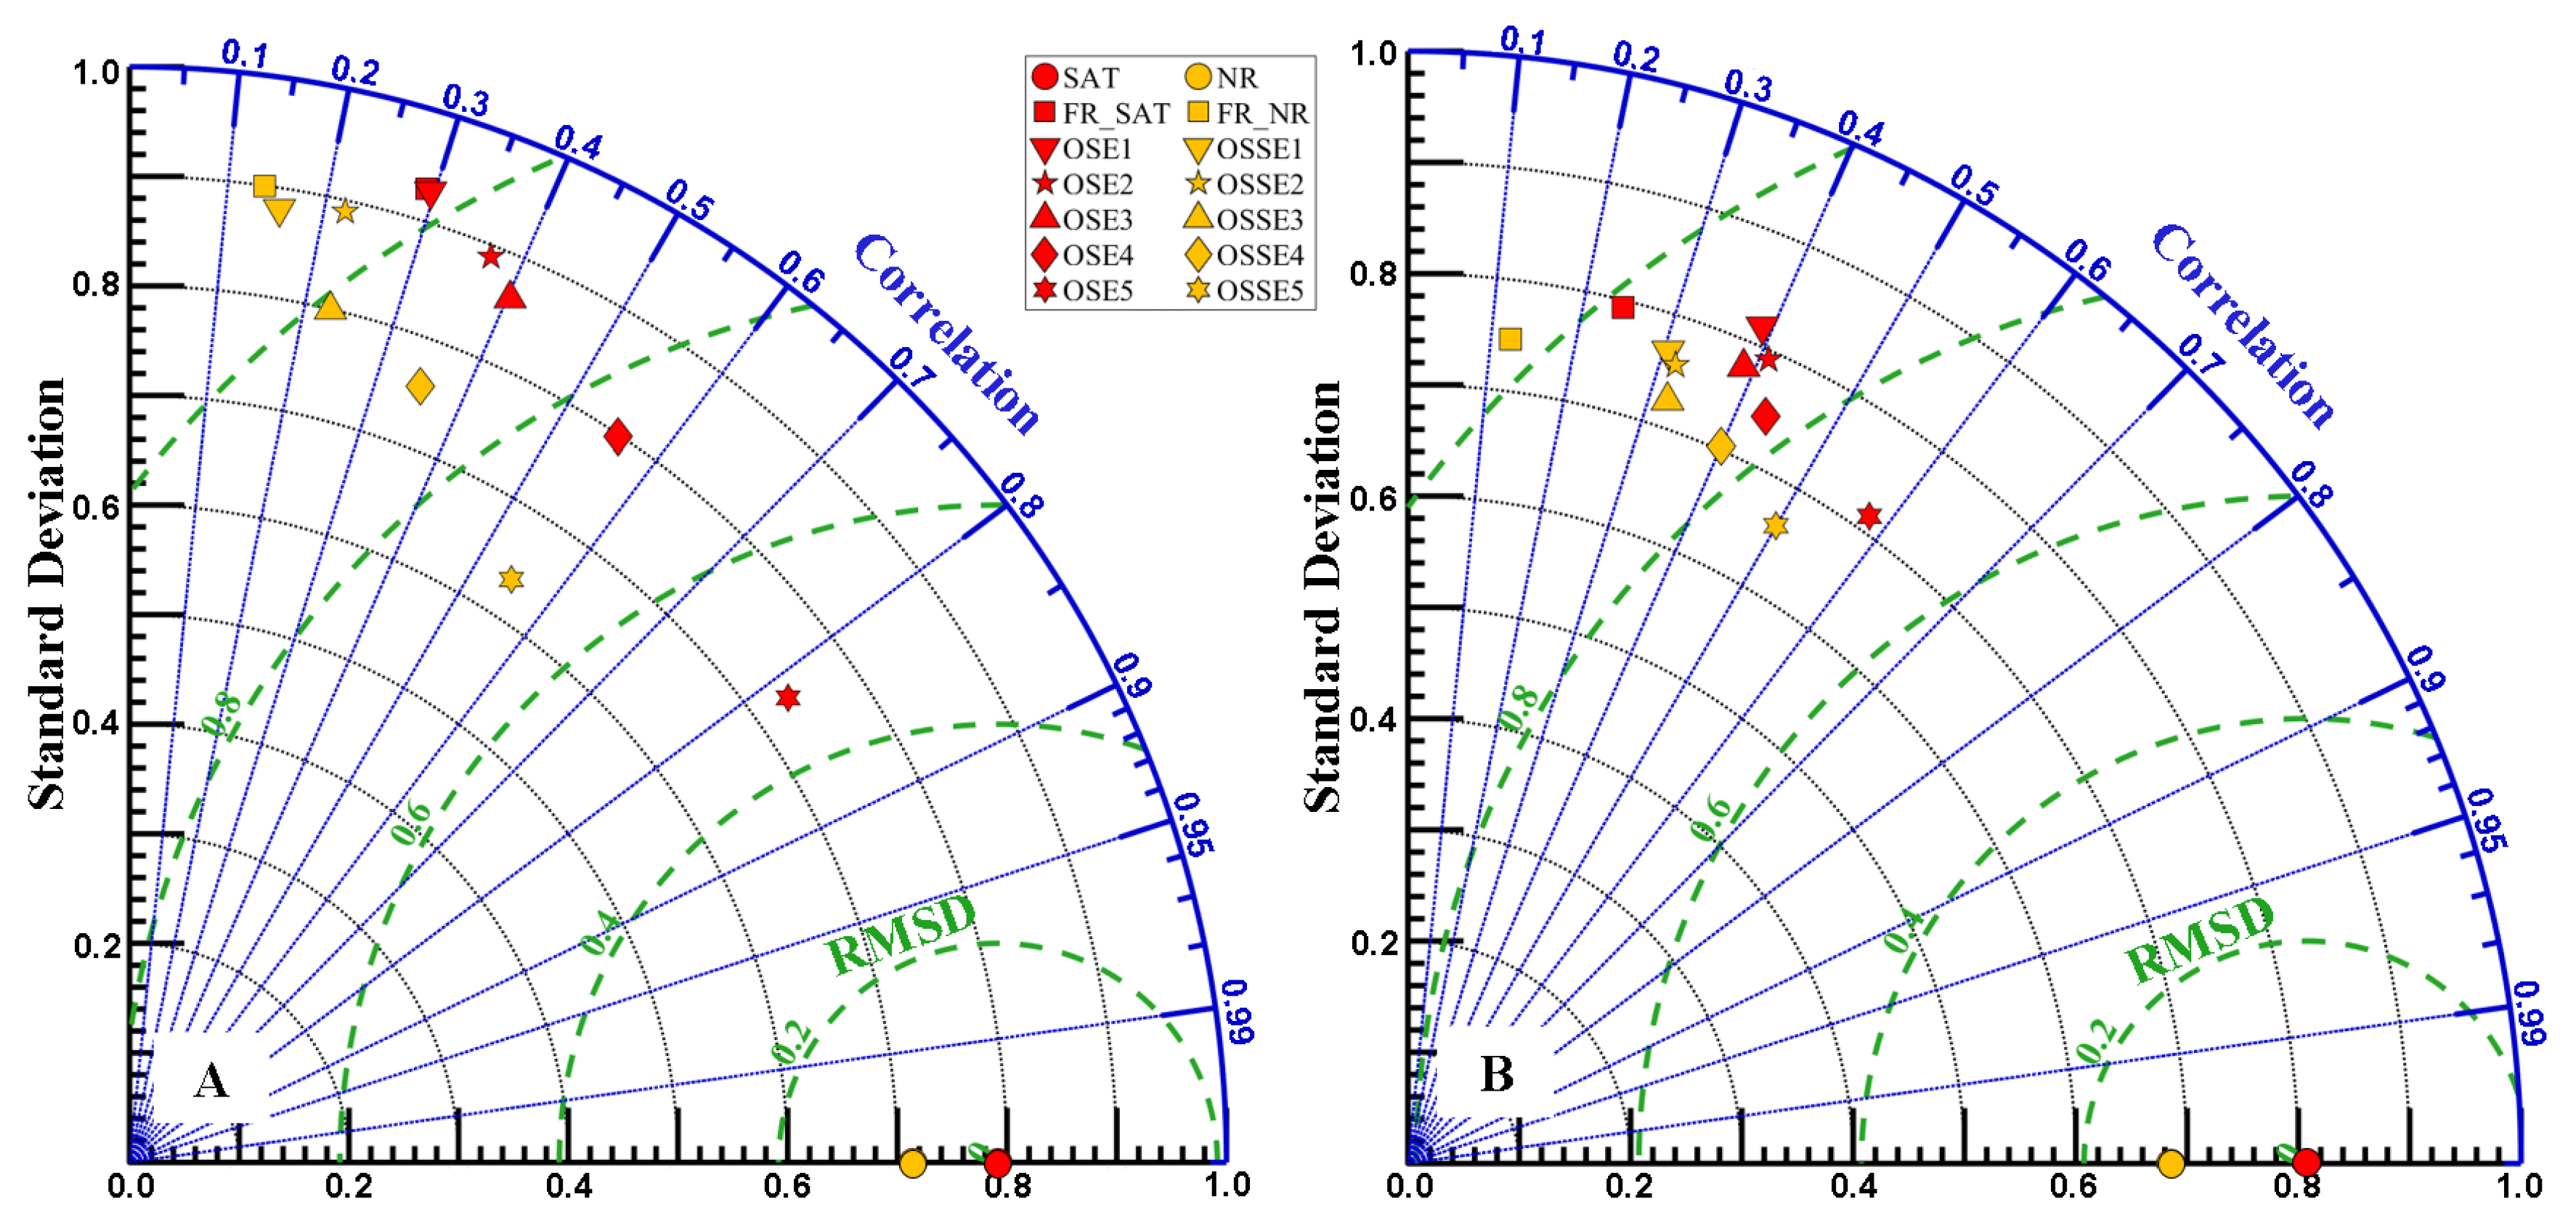
\includegraphics[width=16.0cm]{figures/fig2.7.png}
    \caption{The Taylor diagrams present the statistical properties (standard deviation, correlation, and root mean square difference, RMSD) for OSE1-OSE5 and OSSE1-OSSE5, as well as the Free Run (FR\_SAT) relative to the NRT ODYSSEA satellite data (SAT) and the Free Run (FR\_NR) relative to the Nature Run (NR). Panel~(\textbf{A}) shows the results immediately after the EnOI update, and Panel~(\textbf{B}) shows the results seven days later.}
    \label{fig:taylornrt_2.7}
\end{figure}

Finally, an additional metric was used to further assess the system's behaviour: the Murphy Skill Score (MSS), as defined in \bCref{eq:cp2_murphyss}. For the OSE experiments, the NR values in the equation were replaced by the corresponding satellite product, which served as the observational reference. In the OSSE experiments, the NR values remained the reference dataset, reflecting the synthetic nature of these experiments. The results for the experiments based on the NRT ODYSSEA satellite product are shown in \bCref{fig:murphy_2.8}. Each panel illustrates how the MSS varies with the number of assimilated observation points, with the left panel representing the moment immediately after the EnOI update (3 February) and the right panel representing the results from the sampling seven days later (10 February).

As expected, the skill score generally increases as more observations are assimilated, indicating enhanced forecast accuracy. More importantly, the OSSE curves follow the same upward trend as their OSE counterparts, reaffirming the system's consistency. The analysis MSS increases even when a large number of data points is assimilated, whereas the forecast MSS is less sensitive to the number of observations, possibly being hampered by the quality of other inputs, such as lateral and surface boundary conditions. No specific benchmark value for the MSS was sought; rather, the objective was to confirm that OSSE experiments respond similarly to OSEs in terms of performance improvement. Overall, the results demonstrate that the OSSE system developed in this study is internally consistent, sensitive to observation density, and capable of realistically reproducing the correction patterns expected from real-world assimilation. This provides strong evidence of its suitability for assessing the potential impact of future observational strategies, such as those envisioned under the NAUTILOS initiative.

\begin{figure}[H]
    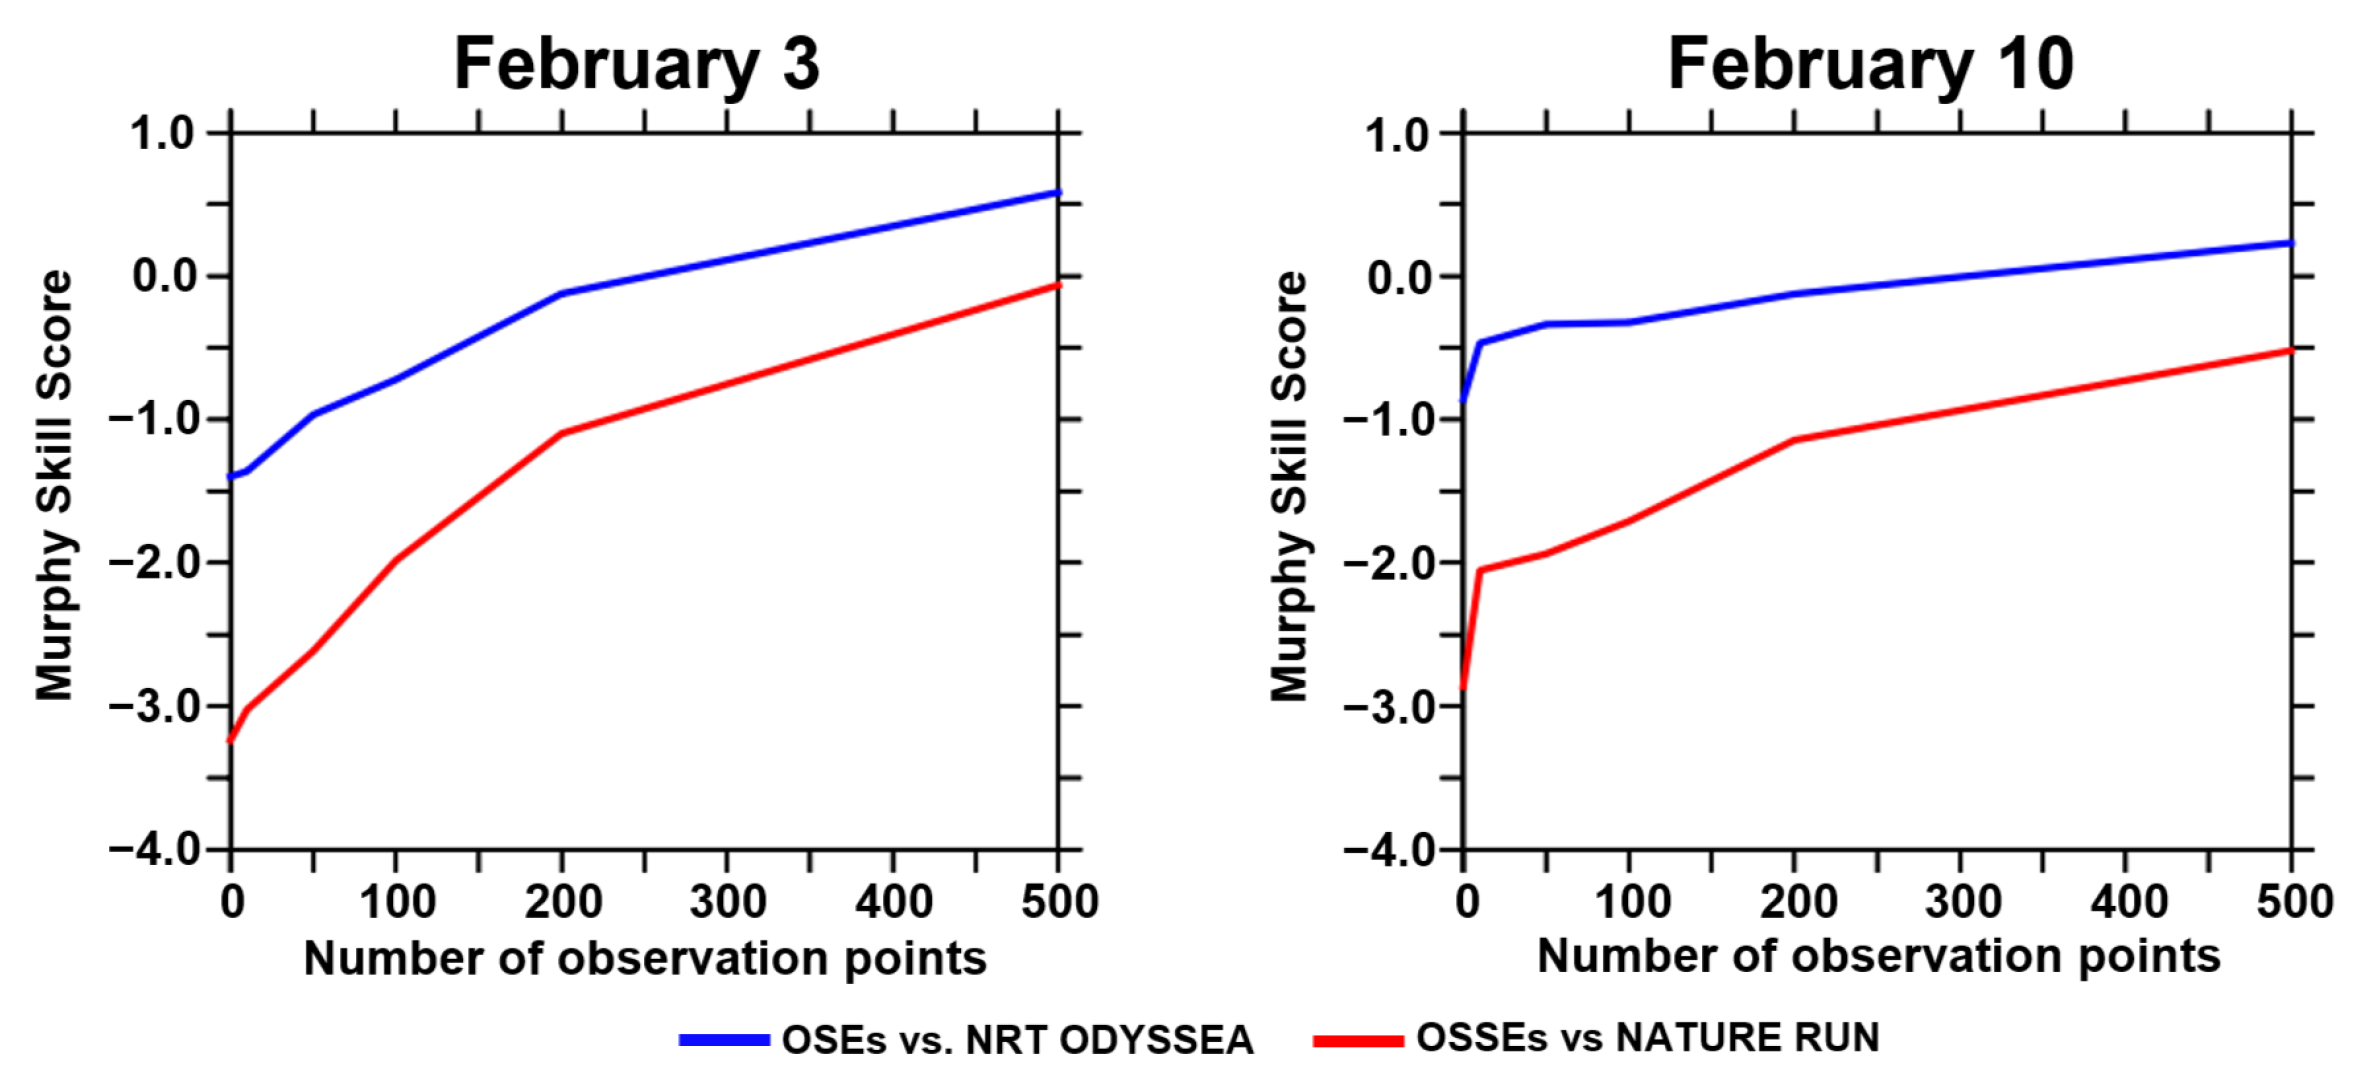
\includegraphics[width=15.0cm]{figures/fig2.8.png}
    \caption{Murphy Skill Score (MSS) for experiments based on the NRT ODYSSEA satellite product. Blue lines indicate OSE experiments, with skill scores computed relative to their satellite-based reference data; red lines indicate OSSE experiments, computed relative to the NR. The left panel shows MSS immediately after the EnOI update (3 February), and the right panel shows MSS seven days later (10 February).}
    \label{fig:murphy_2.8}
\end{figure}

\section{Conclusions} \label{sec:ossedesign_conclude}
A practical framework for assessing the possible influence of new observation systems on model forecasts before their actual deployment is provided by Observation System Simulation Experiments (OSSEs). Within this context, the main objective of this study was to design and validate an OSSE system tailored to the operational model of the Algarve coast, SOMA. The system was developed using the fraternal twins approach, in which two configurations of the same model, MOHID, were used to simulate the Nature Run (NR) and the Forecast Model (FM).

In the NR, SOMA's original operational configuration was used. In contrast, the FM was modified to a lower-resolution grid and did not include weekly adjustments from outer conditions. For this reason, the FM was also referred to as the Free Run (FR) in the proposed OSSE system. Data assimilation was carried out using the EnOI scheme, which was chosen for its balance between computational efficiency and representativeness of ensemble-based statistics. At this stage, assimilation was limited to surface observations, both due to the current configuration of the DA system, which still requires further adaptation to support 3D assimilation with SOMA, and to ensure consistency with the operational satellite-based products used in the Observing System Experiments (OSEs).

As recommended in the literature, an OSSE system should be evaluated against a comparable OSE system in order to ensure that the former does not produce unrealistic results when assessing new observations. In this study, such a comparison was made using two distinct L4 satellite products for SST from CMEMS: the NRT ODYSSEA product and the Reprocessed dataset. These products served as references for the OSE experiments, while the corresponding OSSEs assimilated synthetic SST observations derived from the NR. The results confirmed that the OSSE system responded consistently across both satellite references, as demonstrated by the RMSE evolution over time, Taylor diagrams, and Murphy Skill Score; these results support its robustness and reliability for future impact assessments.

A key aspect of the methodology is the emulation of realistic observational errors in the synthetic data, which ensures that the assessment of new data streams reflects the uncertainties of real-world applications. This was achieved by generating pseudo-random fields, using a spatial correlation factor across the NR grid, and scaling by satellite-derived error data. The result is a flexible framework that preserves the statistical structure of real observation errors and can be used to test different error magnitudes in the future. Although the experiments presented were tailored to SOMA and the Algarve region, the methodological framework is not tied to SOMA specifically. The generation of synthetic observations and their associated error fields allows for straightforward transfer to other coastal models and regional contexts, broadening the model's applicability and making it useful as a base model for evaluating emerging observing systems beyond that presented in the present case study. 

The results presented here indicate that the SOMA OSSE system is consistent, sensitive to the number of observations used in the update step, and capable of realistically emulating synthetic observation errors. As such, it provides a solid foundation for future studies aimed at assessing the impact of emerging observation strategies in the Algarve region, including those being developed under the NAUTILOS project. Beyond its immediate application, the system also paves the way to broader developments, such as more in-depth research into the correlation between the SST and salinity state variables of the model, which could enhance the system's robustness by enabling more advanced multivariate assimilation strategies.

This work also constitutes a very significant milestone in SOMA's operational forecasts: the adaptation and integration of a DA system to improve the model state variables, including real satellite observations. However, the restriction to surface-only assimilation remains a critical limitation of the current system. Future developments should prioritize the integration of the EnOI scheme with real-time forecasts and the expansion of its scope to encompass additional observation types, such as satellite altimetry and 3D in situ fields like those obtained by autonomous platforms, including the AUV missions already operational in the region \parencite{cima2024soma}. In addition, a systematic sensitivity analysis of the weighting coefficient $\alpha$ will be an essential step in optimizing the balance between background error structures and observational impact, ensuring a more robust assimilation framework. In this sense, the present study should be seen as a first step in the development of a more comprehensive DA framework that will culminate in a significant enhancement of the operational monitoring capacity along the Algarve coast.

\section{Supplementary Materials} \label{sec:cp2_supp}
\begin{figure}[H]
   \centering
   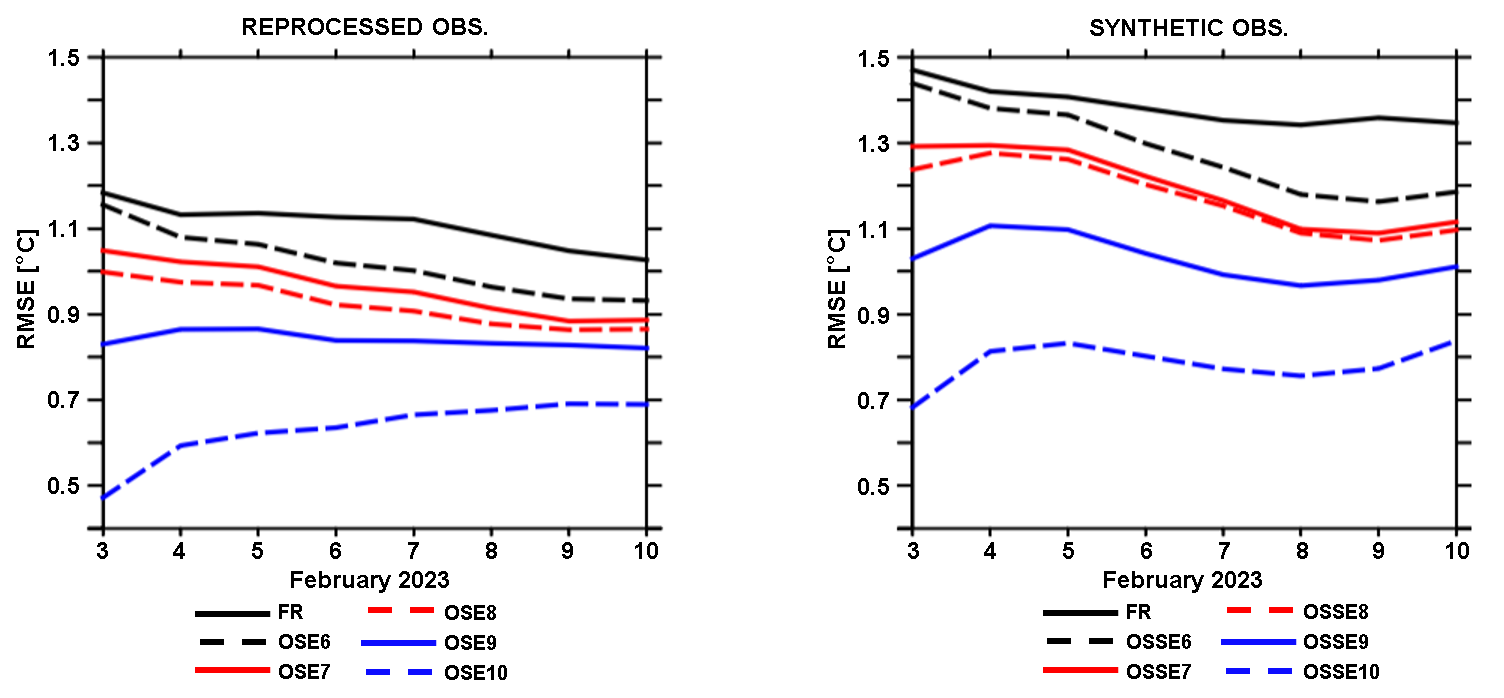
\includegraphics[width=15.0cm]{figures/fig2.9.png}
   \caption{On the left, the SST error over time of the FR and experiments OSE6 to OSE10, referenced in \bCref{tab:exps_2.1}, with respect to the Reprocessed satellite product. On the right, the SST error of the FR and experiments OSSE6 to OSSE10 with respect to the NR. The experiments were integrated for an additional seven days following the update on 3 February.}
   \label{fig:rmserep_2.9}
\end{figure}


\section{Data Availability Statement}
The operational data from the Algarve modelling system (SOMA) are openly available at \href{https://doi.org/10.34623/tx0z-bb23}{https://doi.org/10.34623/tx0z-bb23}.

\section{Appendix A} \label{sec:ossedesign_appxA}
This appendix details the core metrics used to evaluate the Forecast Model (FM) against the Nature Run (NR). The same equations are applied to assess (1) the FM against actual observation data, (2) OSSE experiments against the NR, and (3) OSE experiments against observational data.

\subsection{Spatially Integrated Averages and Standard Deviations}
A straightforward comparison between the models can be accomplished by calculating the instantaneous spatial averages (\textit{AVG}) and standard deviations (\textit{STD}) of the NR and FM. The resulting data can then be utilized to construct a time series of model evolution. The parameters are defined as follows:

\begin{equation}\label{eq:cp2_avg}
	AVG(t_{i}) = \frac{\Sigma_{\text{domain}}\theta(t_{i})}{N},
\end{equation}
\begin{equation}\label{eq:cp2_std}
	STD(t_{i}) = \sqrt{\frac{\Sigma_{\text{domain}} \Bigl( \theta(t_{i})-AVG(t_{i}) \Bigr)^2}{N}}.
\end{equation}

In the previous equations, $\theta$ is the analyzed variable at time $t_i$, and $N$ the number of grid cells. Values can represent instantaneous outputs or averages within a time window centered on $t_i$, with both the window length and sampling frequency (e.g., daily or weekly) depending on the process and region. Spatial sums may cover the full 3D field or a chosen 2D layer, such as the surface. The time series obtained from \textit{AVG} (\bCref{eq:cp2_avg}) and \textit{STD} (\bref{eq:cp2_std}) offer a straightforward means of comparing the FM against the NR through time. The same diagnostics can be extended to observational datasets (e.g., L4 SST or SSH data products), ensuring that the model's statistical behaviour is consistent with real-world conditions.

\subsection{Spatially Integrated RMSE}
The time series of the instantaneous spatially integrated root mean square error (\textit{RMSE}) is an effective preliminary indicator of the forecast evolution in relation to the NR and observations. This parameter is defined by the following equation:

\begin{equation}\label{eq:cp2_rmse}
	RMSE(t_i) = \sqrt{\frac{\Sigma_\text{domain} \Bigl( \theta_{FM}(t_i) - \theta_{NR}(t_i) \Bigr)^2}{N}}.
\end{equation}

In the last equation, $\theta_{NR}$ and $\theta_{FM}$ represent the variables from the Nature Run and the Forecast Model, respectively, at time $t_i$, while $N$ is the number of grid cells considered. As with \textbf{Equations}~\bref{eq:cp2_avg} and~\bref{eq:cp2_std}, $\theta$ may correspond either to instantaneous outputs or to averages within a time interval centred on $t_i$, with the choice of interval and sampling frequency (e.g., daily or weekly) depending on the process and region under study. The spatial integration can also be carried out over the full 3D domain or restricted to a 2D layer. Since the NR often employs a finer spatial resolution than the FM does to reduce the risk of the \textit{identical twins} problem, it is standard practice to average the NR fields onto the FM grid prior to computing \textit{RMSE}.

\subsection{Temporally Integrated Averages and Standard deviations}
The previous indicators provide a global overview of the temporal evolution of the solutions, yet they do not allow a spatial evaluation. To address this limitation, temporally integrated indicators for each grid point can be employed. The temporally integrated average is computed as follows:

\begin{equation}\label{eq:cp2_avgt}
    AVG(i,j,k) = \frac{\sum_{t_i=0}^{T}\theta(i,j,k)}{N},
\end{equation}

\noindent where $\theta$ denotes the analysed variable, either from the Forecast Model or the NR, evaluated at grid point $(i,j,k)$, while $T$ is the number of time steps included. The values of $\theta$ may correspond to instantaneous outputs or to averages over a time interval centred on $t_i$. Using the same approach, the standard deviation can be derived according to \bCref{eq:cp2_stdt}:

\begin{equation}\label{eq:cp2_stdt}
    STD(i,j,k) = \sqrt{\frac{\sum_{t_i=0}^{T} \Bigl( \theta(i,j,k) - AVG(i,j,k) \Bigr)^2}{N}}.
\end{equation}

Horizontal and vertical maps can be plotted from the indicators in \textbf{Equations}~\bref{eq:cp2_avgt} and~\bref{eq:cp2_stdt}, which provide a general idea of the spatial behaviour of the model statistics.

\subsection{Temporally Integrated RMSE}
The temporally integrated \textit{RMSE} between the forecast and the reference NR can be calculated using the same logic employed for the previous indicators. This allows the plotting of horizontal maps of each layer or vertical cuts, which provide a general overview of the spatial distribution of forecast deviations relative to the NR. It is computed by the following:

\begin{equation}\label{eq:cp2_rmset}
    RMSE(t_i) = \sqrt{\frac{\sum_{t_i=0}^{T} \Bigl( \theta_{FM}(i,j,k) - \theta_{NR}(i,j,k) \Bigr)^2}{N}}.
\end{equation}

\subsection{Murphy Skill Score}
The metrics described in \Cref{sec:ossedesign_appxA} provide a general characterization of the NR and FM and a simple way to compare them. However, the literature also recommends the use of more sophisticated statistical metrics, such is the Murphy Skill Score (\textit{MSS}):

\begin{equation}\label{eq:cp2_murphyss}
    MSS = \rho^2 - \left[ \rho - \frac{\sigma_{FM}}{\sigma_{NR}} \right]^2 - \left[ \frac{\overline \theta_{FM}-\overline \theta_{NR}}{\sigma_{NR}} \right]^2.
\end{equation}

The \textit{MSS} can be evaluated either over the full grid or individually at each grid cell for a selected time period, thereby yielding a spatial distribution of predictive performance. In \bCref{eq:cp2_murphyss}, $\rho$ is the correlation between the NR and FM, $\sigma$ is the standard deviation, and $\overline{\theta}$ represents the average of the variable analysed. Following \textcite{murphy1988skill}, \textit{MSS} values vary between $-\infty$ and 1: a score of 1 corresponds to a perfect forecast, 0 indicates no improvement relative to the reference, and negative values denote performance worse than that of the reference. Intermediate values $(0 < MSS < 1)$ indicate increasing levels of forecast improvement.

\subsection{Taylor Diagrams} \label{subsec:cp2_taylor}
The Taylor Diagram \parencite{taylor2001summarizing} is a graphical tool developed to summarize the performance of models by combining three statistical metrics---correlation, root mean square difference (\textit{RMSD}), and standard deviation---into a single and interpretable plot. It provides a compact way to visualize and compare the agreement between the forecast output and the reference NR, where each comparison (or each OSSE) is represented as a point on a polar coordinate system. The azimuthal position of each point reflects the correlation between FM and NR, while the radial distance from the origin represents the pattern's standard deviation, and the distance from the reference point shows the RMSD. Thus, the diagram offers a rapid method of evaluating the accuracy of the forecast model.

The distinction between \textit{RMSE} and \textit{RMSD} lies in their respective focuses. \textit{RMSE} is a broader measure of overall accuracy, capturing both the mean difference (bias) and variability between the forecast and NR. In contrast, \textit{RMSD} removes the bias first, allowing it to emphasize discrepancies in the shape and phase of the spatial or temporal structure and variability of the dataset. Thus, it is defined by the following equation:

\begin{equation}\label{eq:cp2_rmsd}
    RMSD = \sqrt{\frac{\sum_{i=1}^N \Bigl( (\theta_{FM_i} - \overline\theta_{FM}) - (\theta_{NR_i} - \overline\theta_{NR}) \Bigr)^2}{N}},
\end{equation}

\noindent where $\theta$ is the analysed variable in FM and NR; $\overline\theta$ is the average of that variable; and $N$ is the number of grid cells used. In general, the closer the forecast result is to the NR, the better the model performance.
 
\section{Appendix B} \label{sec:ossedesign_appxB}
The general formulation of the Ensemble Optimal Interpolation (EnOI) can be introduced through the standard analysis equation of a Data Assimilation (DA) problem, expressed in \textbf{Equations}~(\bref{eq:cp2_daprob}) and~(\bref{eq:cp2_daK}), where the time index is omitted for clarity:

\begin{equation}\label{eq:cp2_daprob}
	\mathbf{x}^a=\mathbf{x}^b+\mathbf{K} \left( \mathbf{y}-\mathbf{Hx}^b \right),
\end{equation}

\begin{equation}\label{eq:cp2_daK}
	\mathbf{K}=\mathbf{PH}^T \left[ \mathbf{HPH}^T+\mathbf{R} \right]^{-1}.
\end{equation}

\bCref{eq:cp2_daprob} provides the model state update in $\mathbf{x}^a$. The current state of the model, or the background, is denoted by $\mathbf{x}^b$ and, together with the analysis, they are m-dimensional vectors of real numbers, i.e., $\left( \mathbf{x}^a,\mathbf{x}^b \right) \in \mathbb{R}^m$. The state vectors typically contain the values at all grid cells of all variables being updated in the assimilation process, such as velocity components, temperature, salinity, or SSH, although the specific variables included depend on the configuration and objectives of the system. The observation vector is given by $\mathbf{y} \in \mathbb{R}^d$ and $\mathbf{H} \in \mathbb{R}^{d \times m}$ is a matrix which serves as an operator to map the background vector to the observations' space.

In \bCref{eq:cp2_daK} the superscripts $^T$ indicate a transposed matrix, $\mathbf{K} \in \mathbb{R}^{m \times d}$ is the matrix of weights, akin to the Kalman gain in the Ensemble Kalman Filter (EnKF), $\mathbf{P} \in \mathbb{R}^{m \times m}$ is the background error covariance matrix, and $\mathbf{R} \in \mathbb{R}^{d \times d}$ is the observation error covariance matrix. From the two equations and in the event that the uncertainty associated with the model is significantly smaller than that associated with the observations (i.e., $\mathbf{P}<<\mathbf{R}$), the weights approach zero. Consequently, the analysis in \bCref{eq:cp2_daprob} practically becomes the value of the background. Conversely, if the observations are more reliable than the model (i.e., $\mathbf{R}<<\mathbf{P}$), then more weight is given to the observations.

If the analysis equation is to be solved, some definitions must be given. Firstly, the matrix holding the static ensemble members of the background is given by $\mathbf{E}$ in \bCref{eq:cp2_ensemble}:

\begin{equation}\label{eq:cp2_ensemble}
	\mathbf{E}=\left( \mathbf{x_1},\mathbf{x_2},\cdots,\mathbf{x_N} \right)\in\mathbb{R}^{m\times N},
\end{equation}

\noindent where $N$ is the number of ensemble members, each one an m-dimensional state vector. With that, the ensemble anomaly ($\mathbf{X'}$) is defined as the following:

\begin{equation}\label{eq:cp2_anomaly}
	\mathbf{X'}=\mathbf{E}-\overline{\mathbf{E}},
\end{equation}

\noindent where $\overline{\mathbf{E}}$ is the ensemble mean. Then, the ensemble covariance matrix $\mathbf{P}$ can be defined as

\begin{equation}\label{eq:cp2_encov}
	\mathbf{P}=\frac{\mathbf{X'X'}^{T}}{N-1}.
\end{equation}

Moving to the measurements vector $\mathbf{y}$ in \bCref{eq:cp2_daprob}, an ensemble of perturbed observations must be introduced into the system to ensure that the ensemble analysis properly accounts for the measurement uncertainty and maintains consistency with the computation of the Kalman gain. The perturbation is defined by \bCref{eq:cp2_enobs}:

\begin{equation}\label{eq:cp2_enobs}
	\mathbf{y_i}=\mathbf{y}+\epsilon_i, \quad 1\leq i\leq N,
\end{equation}

\noindent where $\epsilon_i$ is the simulated random measurement error, drawn from a distribution with zero mean and a covariance that matches the observation error covariance matrix $\mathbf{R}$ in \bCref{eq:cp2_daK}. In this way, the perturbed observations can be stored in the following observation matrix:

\begin{equation}\label{eq:cp2_obspertub}
    \mathbf{Y}=\left( \mathbf{y_1},\mathbf{y_2},\cdots,\mathbf{y_N} \right)\in\mathbb{R}^{d\times N}.
\end{equation}

With the previous statements, it is possible to replace the error covariance matrices in the analysis $\mathbf{x}^a$ and in $\mathbf{K}$ by their ensemble representation to obtain the ensemble of updated states ($\mathbf{E}^a$):

\begin{equation}\label{eq:cp2_enkf}
    \mathbf{E}^a=\mathbf{E} + \mathbf{X'X'}^T \mathbf{H}^T \left[ \mathbf{HX'X'}^T \mathbf{H}^T +(N-1) \mathbf{R}\right]^{-1} \left( \mathbf{Y}-\mathbf{HE} \right).
\end{equation}

\bCref{eq:cp2_enkf} shows the general formulation of the EnKF analysis scheme, which includes updating each member of the ensemble and integrating the model $N$ times to calculate the error covariance matrix $\mathbf{P}$. However, in the EnOI, the analysis is computed only for one single model state, so the last equation can be rewritten as follows:

\begin{equation}\label{eq:cp2_enoi}
    \mathbf{x}^a=\mathbf{x}^b + \alpha\mathbf{X'X'}^T \mathbf{H}^T \left[ \alpha\mathbf{HX'X'}^T \mathbf{H}^T +(N-1) \mathbf{R}\right]^{-1} \left( \mathbf{y}-\mathbf{Hx}^b \right).
\end{equation}

In \bCref{eq:cp2_enoi}, the parameter $\alpha\in(0,1]$ is introduced to tune the weight given to the ensemble background error covariance relative to the observation error covariance \parencite{evensen2003ensemble}. Since EnOI employs a stationary ensemble to approximate background error statistics, the background variance can sometimes be overestimated due to the long-term sampling of model states. The scaling factor $\alpha$ mitigates this issue by reducing the ensemble-based covariance contribution to a level that better represents the actual forecast uncertainty at the time of assimilation. When $\alpha$ approaches zero, the effective observation error variance is inflated, leading the analysis to converge toward the background state ($\mathbf{x}^a \approx \mathbf{x}^b$). Conversely, as it approaches one, the ensemble covariance is fully retained, allowing the observations to exert a stronger influence on the analysis update.

\chapter{Optimizing Coastal Observation Strategies for a Southwestern Iberian Forecasting System Using Observing System Simulation Experiments} \label{sec:cp3}

TO BE RELEASED....

\vspace{\fill}
\textbf{Article reference}:\\
Mendonça, F., Martins, F. \& Bertino, L. (2026). Optimizing Coastal Observation Strategies for a Southwestern Iberian Forecasting System Using Observing System Simulation Experiments. Submitted to \href{https://www.frontiersin.org/journals/marine-science}{\textit{Frontiers in Marine Science}} (Electronic ISSN 2296-7745) and currently under review.
\newpage

\chapter{SMS-Coastal, a New Python Tool to Manage MOHID-Based Coastal Operational Models} \label{sec:cp4}
\vspace{\fill}
\textbf{Article reference}:\\
Mendonça, F., Martins, F., \& Janeiro, J. (2023). SMS-Coastal, a New Python Tool to Manage MOHID-Based Coastal Operational Models. \textit{Journal of Marine Science and Engineering}, 11(8), 1606. \href{https://doi.org/10.3390/jmse11081606}{https://doi.org/10.3390/jmse11081606}
\clearpage

\section{Abstract}
This paper presents the Simulation Management System for Operational Coastal Hydrodynamic Models, or SMS-Coastal, and its novel methodology designed to automate forecast simulations of coastal models. Its working principle features a generic framework that can be easily configured for other applications, and it was implemented with the Python programming language. The system consists of three main components: the Forcing Processor, Simulation Manager, and Data Converter, which perform operations such as the management of forecast runs and the download and conversion of external forcing data. The SMS-Coastal was tested on two model realisations using the MOHID System: SOMA, a model of the Algarve coast in Portugal, and BASIC, a model of the Cartagena Bay in Colombia. The tool proved to be generic enough to handle the different aspects of the models, being able to manage both forecast cycles.

\vspace{15mm}
\noindent\textbf{Keywords}: operational oceanography; operational modelling; simulation management; ocean forecast; ocean modelling
\vspace{10mm}

\section{Introduction} \label{sec:cp4_intro}
Operational Oceanography refers to a set of activities carried out to observe, describe, and predict the behaviour of the ocean in real-time \parencite{robinson2010introduction, vonschuckmann2016copernicus}. It can be defined as a continuous process involving the collection, interpretation, and dissemination of measured data to analyse the ocean and forecast future conditions \parencite{prandle2000introduction}. The field of operational oceanography consists of two main components \parencite{dombrowsky2011overview}: observation systems, which assess physical and biogeochemical properties through in-situ monitoring and remote sensing \parencite{send2006insitu, ravichandran2011insitu}, and modelling, which utilises ocean data to generate operational models for forecasting and producing data products \parencite{pouliquen2006insitu}.

Ocean modelling is a crucial activity within the scope of operational oceanography \parencite{capet2020operational}. However, modelling coastal areas is particularly challenging due to their high variability, sudden changes, multiple influencing factors, socio-economic activities, data limitations, and scale considerations associated with coastal environments \parencite{she2016developing}. Addressing all these premises requires sophisticated modelling techniques, robust data collection strategies, and a comprehensive understanding of complex coastal dynamics. The Blue Economy, including ocean-related activities, plays a significant role in coastal areas. In Europe, coastal regions are densely populated and contribute more than 30\% to the gross domestic product (GDP) \parencite{she2014analysis}. Therefore, understanding coastal environments is essential, and operational coastal models can provide predictability, generating valuable data that can support sustainable economic growth while ensuring coastal protection \parencite{capet2020operational}.

Operating ocean forecasting models involves a series of routine actions. These actions include downloading forcing data from various suppliers, data processing, cropping, interpolating, formatting, managing simulations, processing, archiving, and disseminating results, among others. Due to the repetitive nature of these tasks, automation is well suited for such operations. Automation systems with similar functionalities are already available for hydrological and watershed applications \parencite{brendel2020integration, lodhi2020urunme, zeng2020development} as well as coastal modelling \parencite{bever2021real, oliveira2020opencoasts, oliveira2021forecasting}. In this context, this article presents a novel software package called the Simulation Management System for Operational Coastal Hydrodynamic Models (SMS-Coastal). This system implements a generic framework designed to automate and manage all the processes involved in an oceanographic forecasting system.

This article is presented as follows: \Cref{sec:cp4_smsc} introduces SMS-Coastal methods, designed to be as generic as possible, allowing their application to operationalise any given forecast model. Later, in \Cref{sec:cp4_results}, results are presented for two examples of operational modelling systems built using the MOHID Modelling System and managed by the proposed tool SMS-Coastal. Discussions and conclusions are presented in \Cref{sec:cp4_discuss} and \Cref{sec:cp4_conclusion}, respectively.

\section{SMS-Coastal Operation} \label{sec:cp4_smsc}
The software package SMS-Coastal represents an innovative solution specifically built to effectively manage the various operations associated with daily simulations in operational oceanographic modelling systems. Developed to operate within the Windows operating system, SMS-Coastal is programmed using Python, a versatile, open-source, high-level, and object-oriented language. Python's extensive collection of adaptable modules and its clean code structure make it highly comprehensible and easily learnable \parencite{saenz2002geophysical}. These factors contribute to Python's popularity, as evidenced by its thriving and rapidly expanding community of users engaged in a wide range of applications, including traditional fields as well as cutting-edge domains such as artificial intelligence, data science, and machine learning \parencite{casanova2020applied}.

Python has gained significant popularity within the scientific community due to its remarkable features, making it highly suitable for ocean modelling \parencite{almeida2011oof}. In addition to its extensive built-in functionalities, Python offers tools designed to handle common data formats used in ocean and atmospheric sciences, such as HDF5, GRIB, and NetCDF. It also provides support for OPeNDAP, tidal harmonic analysis software, and various scientific visualisation resources. The language possesses the necessary capabilities to execute essential tasks involved in maintaining continuous forecast cycles, ensuring the smooth operation of the modelling system. These tasks primarily involve controlling model inputs and outputs. Given these advantageous characteristics, the choice of Python as the programming language for SMS-Coastal is well justified.

As pointed out by \textcite{almeida2011oof}, the execution of a single forecast cycle encompasses several essential steps: (1) Ensuring the availability and retrieval of required external forcing data, which typically include information regarding tides, freshwater discharges, external hydrodynamic fields, atmospheric surface heat and momentum fluxes, among other factors; (2) Effectively managing the archiving of data; (3) Conducting interpolation of external data onto the model grid; (4) Formatting the data to meet the specific requirements of the employed model; (5) Verifying the availability of initial conditions obtained from restart files generated in the preceding simulation cycle; (6) Generating model input files; (7) Performing the simulations; (8) Confirming the completion of the simulations; (9) Managing model outputs and preparing restart files for subsequent forecast cycles; (10) Reformatting, disseminating, and archiving the obtained results; (11) Providing comprehensive reports to the user's supervisor through appropriate messaging channels. Furthermore, daily simulations can quickly produce a large amount of data. To maintain free storage space on the servers, it is highly recommended to define a data archiving policy and create model output databases in different locations or on different devices. It is also advisable to incorporate routine operations to overwrite and/or remove unnecessary input and output data between forecast cycles.

Considering those fundamental steps, SMS-Coastal's most basic architecture was designed with three main components, as shown in \bCref{fig:4.1_smsc}. The first is the Forcing Processor, responsible for downloading all the oceanic and atmospheric external forcing data, conforming it to the model grid (e.g., by interpolation), and formatting it to suitable model file types. The next component is the Simulation Manager, which coordinates forecasts and spin-up simulations and manages the outputs in a local database. The last component is the Data Converter, which is a set of supporting sub-modules that reshape simulation outputs, convert them to a different format, and archive them in a different location. In SMS-Coastal, these three components are completely independent and may be accessed individually. In the next subsections, these components are described in detail.

\subsection{Forcing Processor}
The Forcing Processor has the function of coordinating the operations required to prepare data from other global solutions for the model simulations. Due to the particularities of each data source, it was necessary to create a module in SMS-Coastal that would serve as a library with a set of specific methods appropriate to each data source. Nevertheless, the Forcing Processor main module performs the same generic sequence for all sources, as described by the structure chart in \bCref{fig:4.2_forcing}. In addition to that, it runs the specific methods of that library, which currently supports the data to be used in the operational systems presented in \Cref{sec:cp4_results}, namely: the Operational Mercator global ocean analysis and forecast system from the European Union-Copernicus Marine Service \parencite{cmems2016mercator}; the Skiron from the Atmospheric Modelling and Weather Forecasting Group (AM\&WFG) of the Department of Physics of the National and Kapodistrian University of Athens (NKUA) \parencite{kallos1997regional, papadopoulos2002weather}; and the North American Mesoscale (NAM) Forecast System of the NOAA's National Centres for Environmental Information (NCEP) \parencite{janjic2003nonhydrostatic, janjic2012scientific}.

\begin{figure}[H]
	\centering
    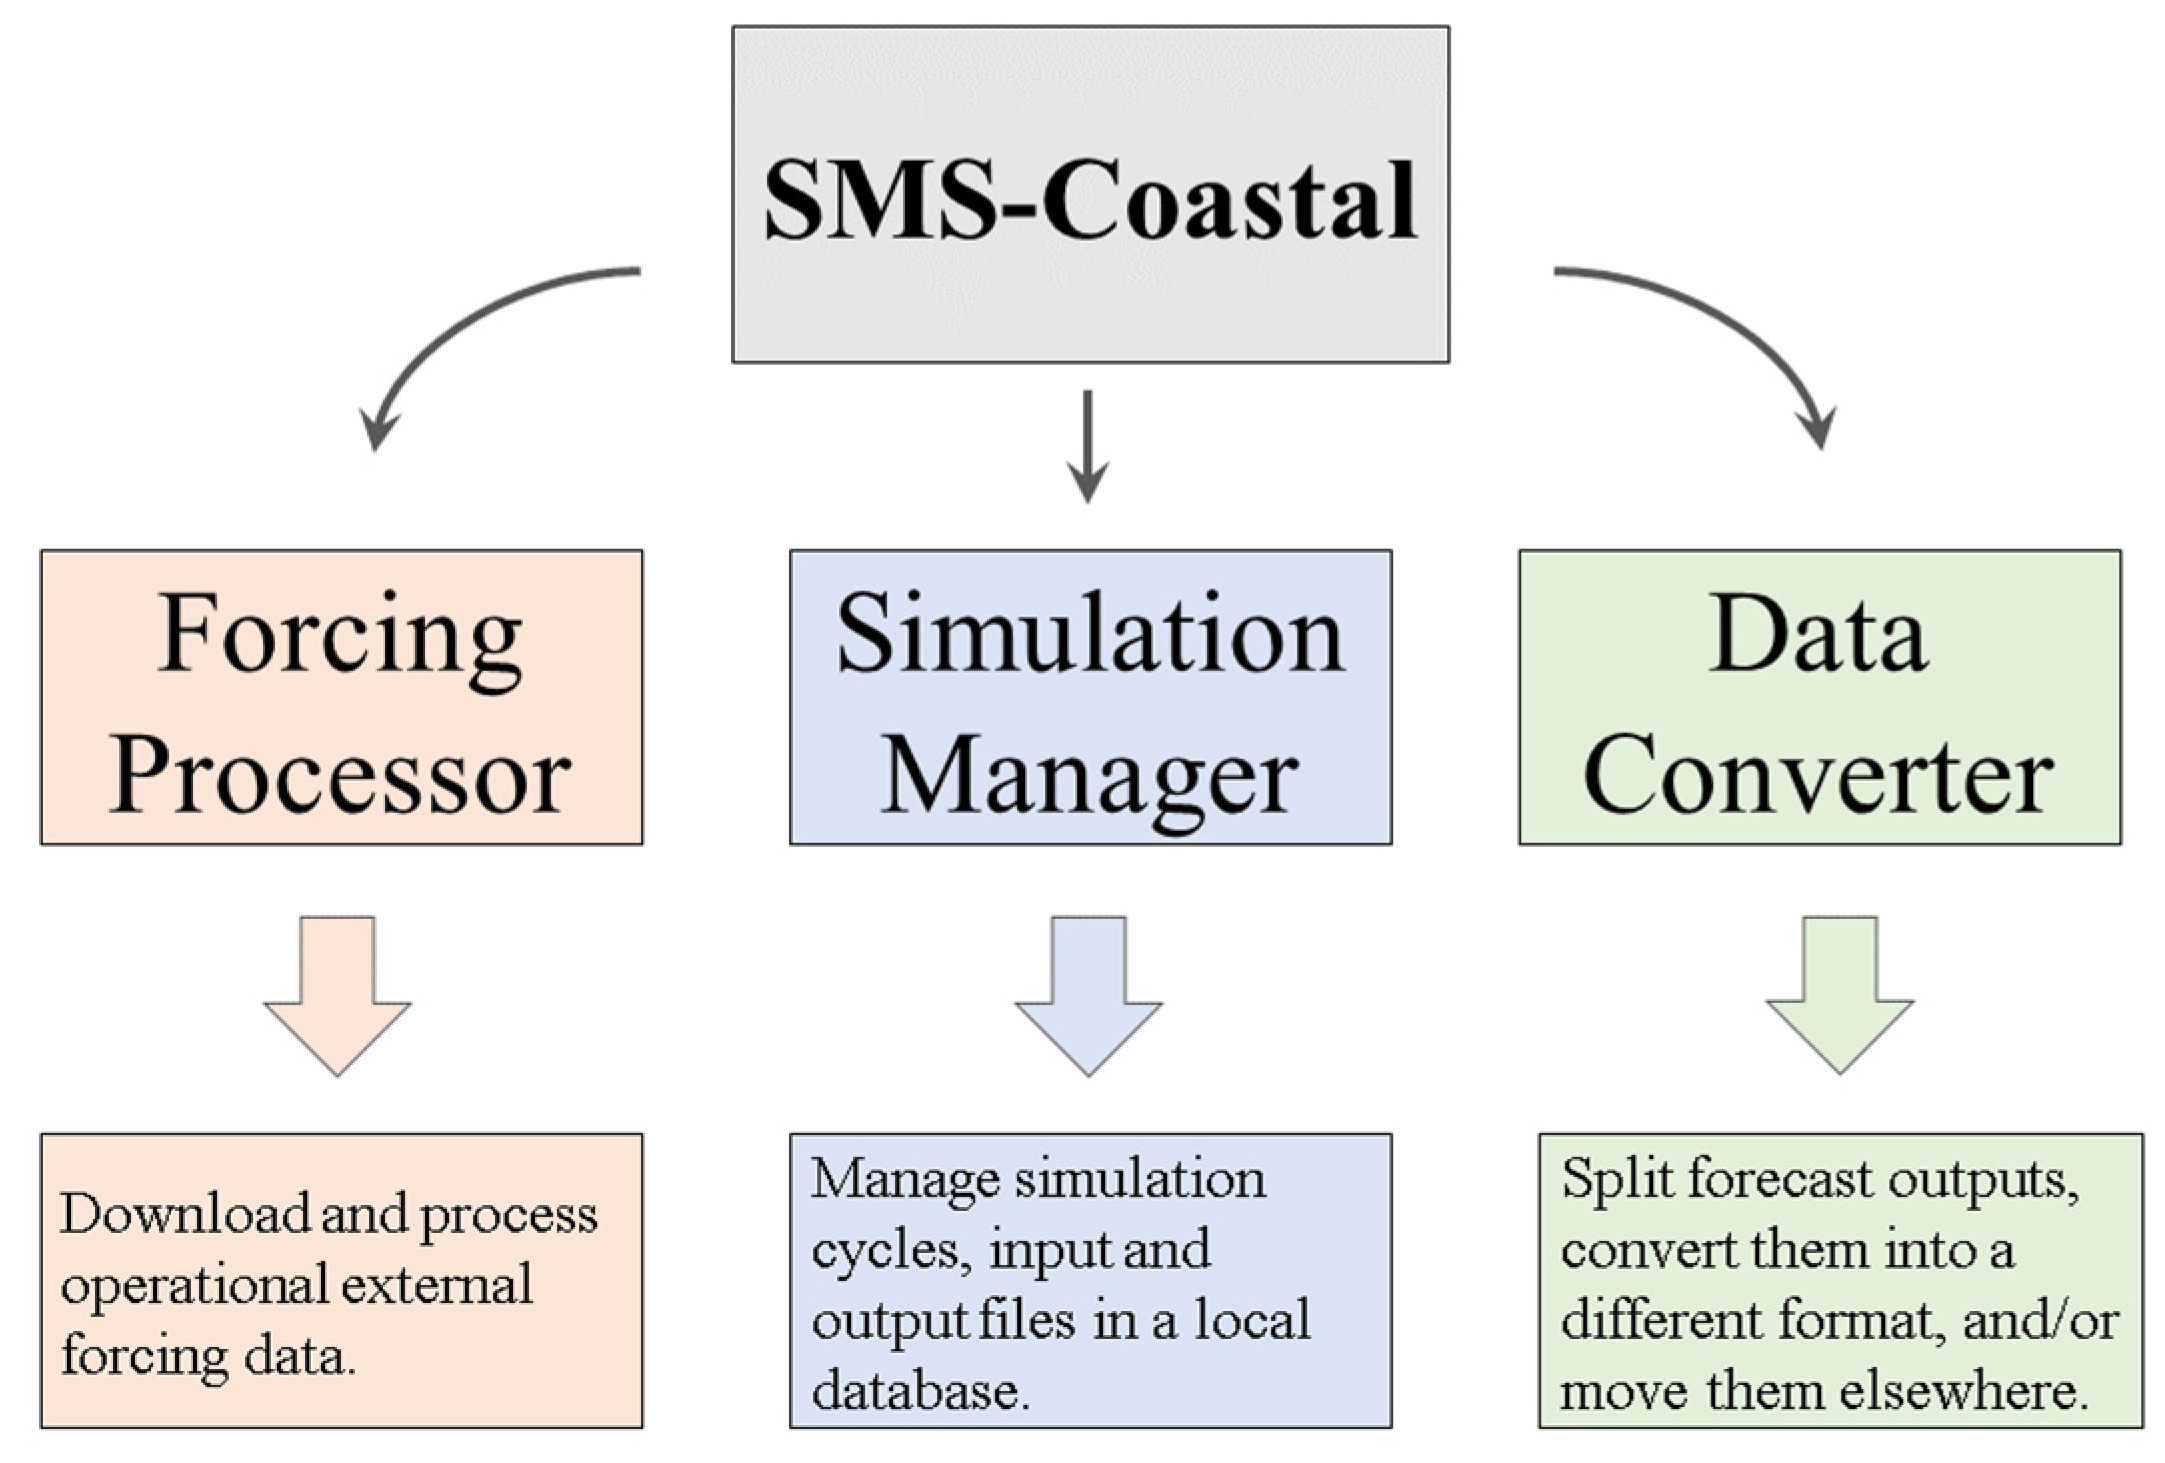
\includegraphics[width=15.0 cm]{figures/fig4.1.png}
    \caption{The three main components of SMS-Coastal are: The Forcing Processor (orange), the Simulation Manager (blue), and the Data Converter (green).}
    \label{fig:4.1_smsc}
\end{figure}

As shown by the operations in \bCref{fig:4.2_forcing}, the process for each data source starts by checking the directory structure on disc. If necessary, SMS-Coastal creates the set of folders and the log file that will be used in the subsequent operations. This structure is fixed and is composed of folders for the download, conversion, interpolation, and simulation data. Except for the last, the tool will overwrite files from a previous run to prevent data accumulation on disc. After this preparation, SMS-Coastal backs up the downloaded files in a different folder if the provider does not maintain a long-term repository.

\begin{figure}[H]
	\centering
    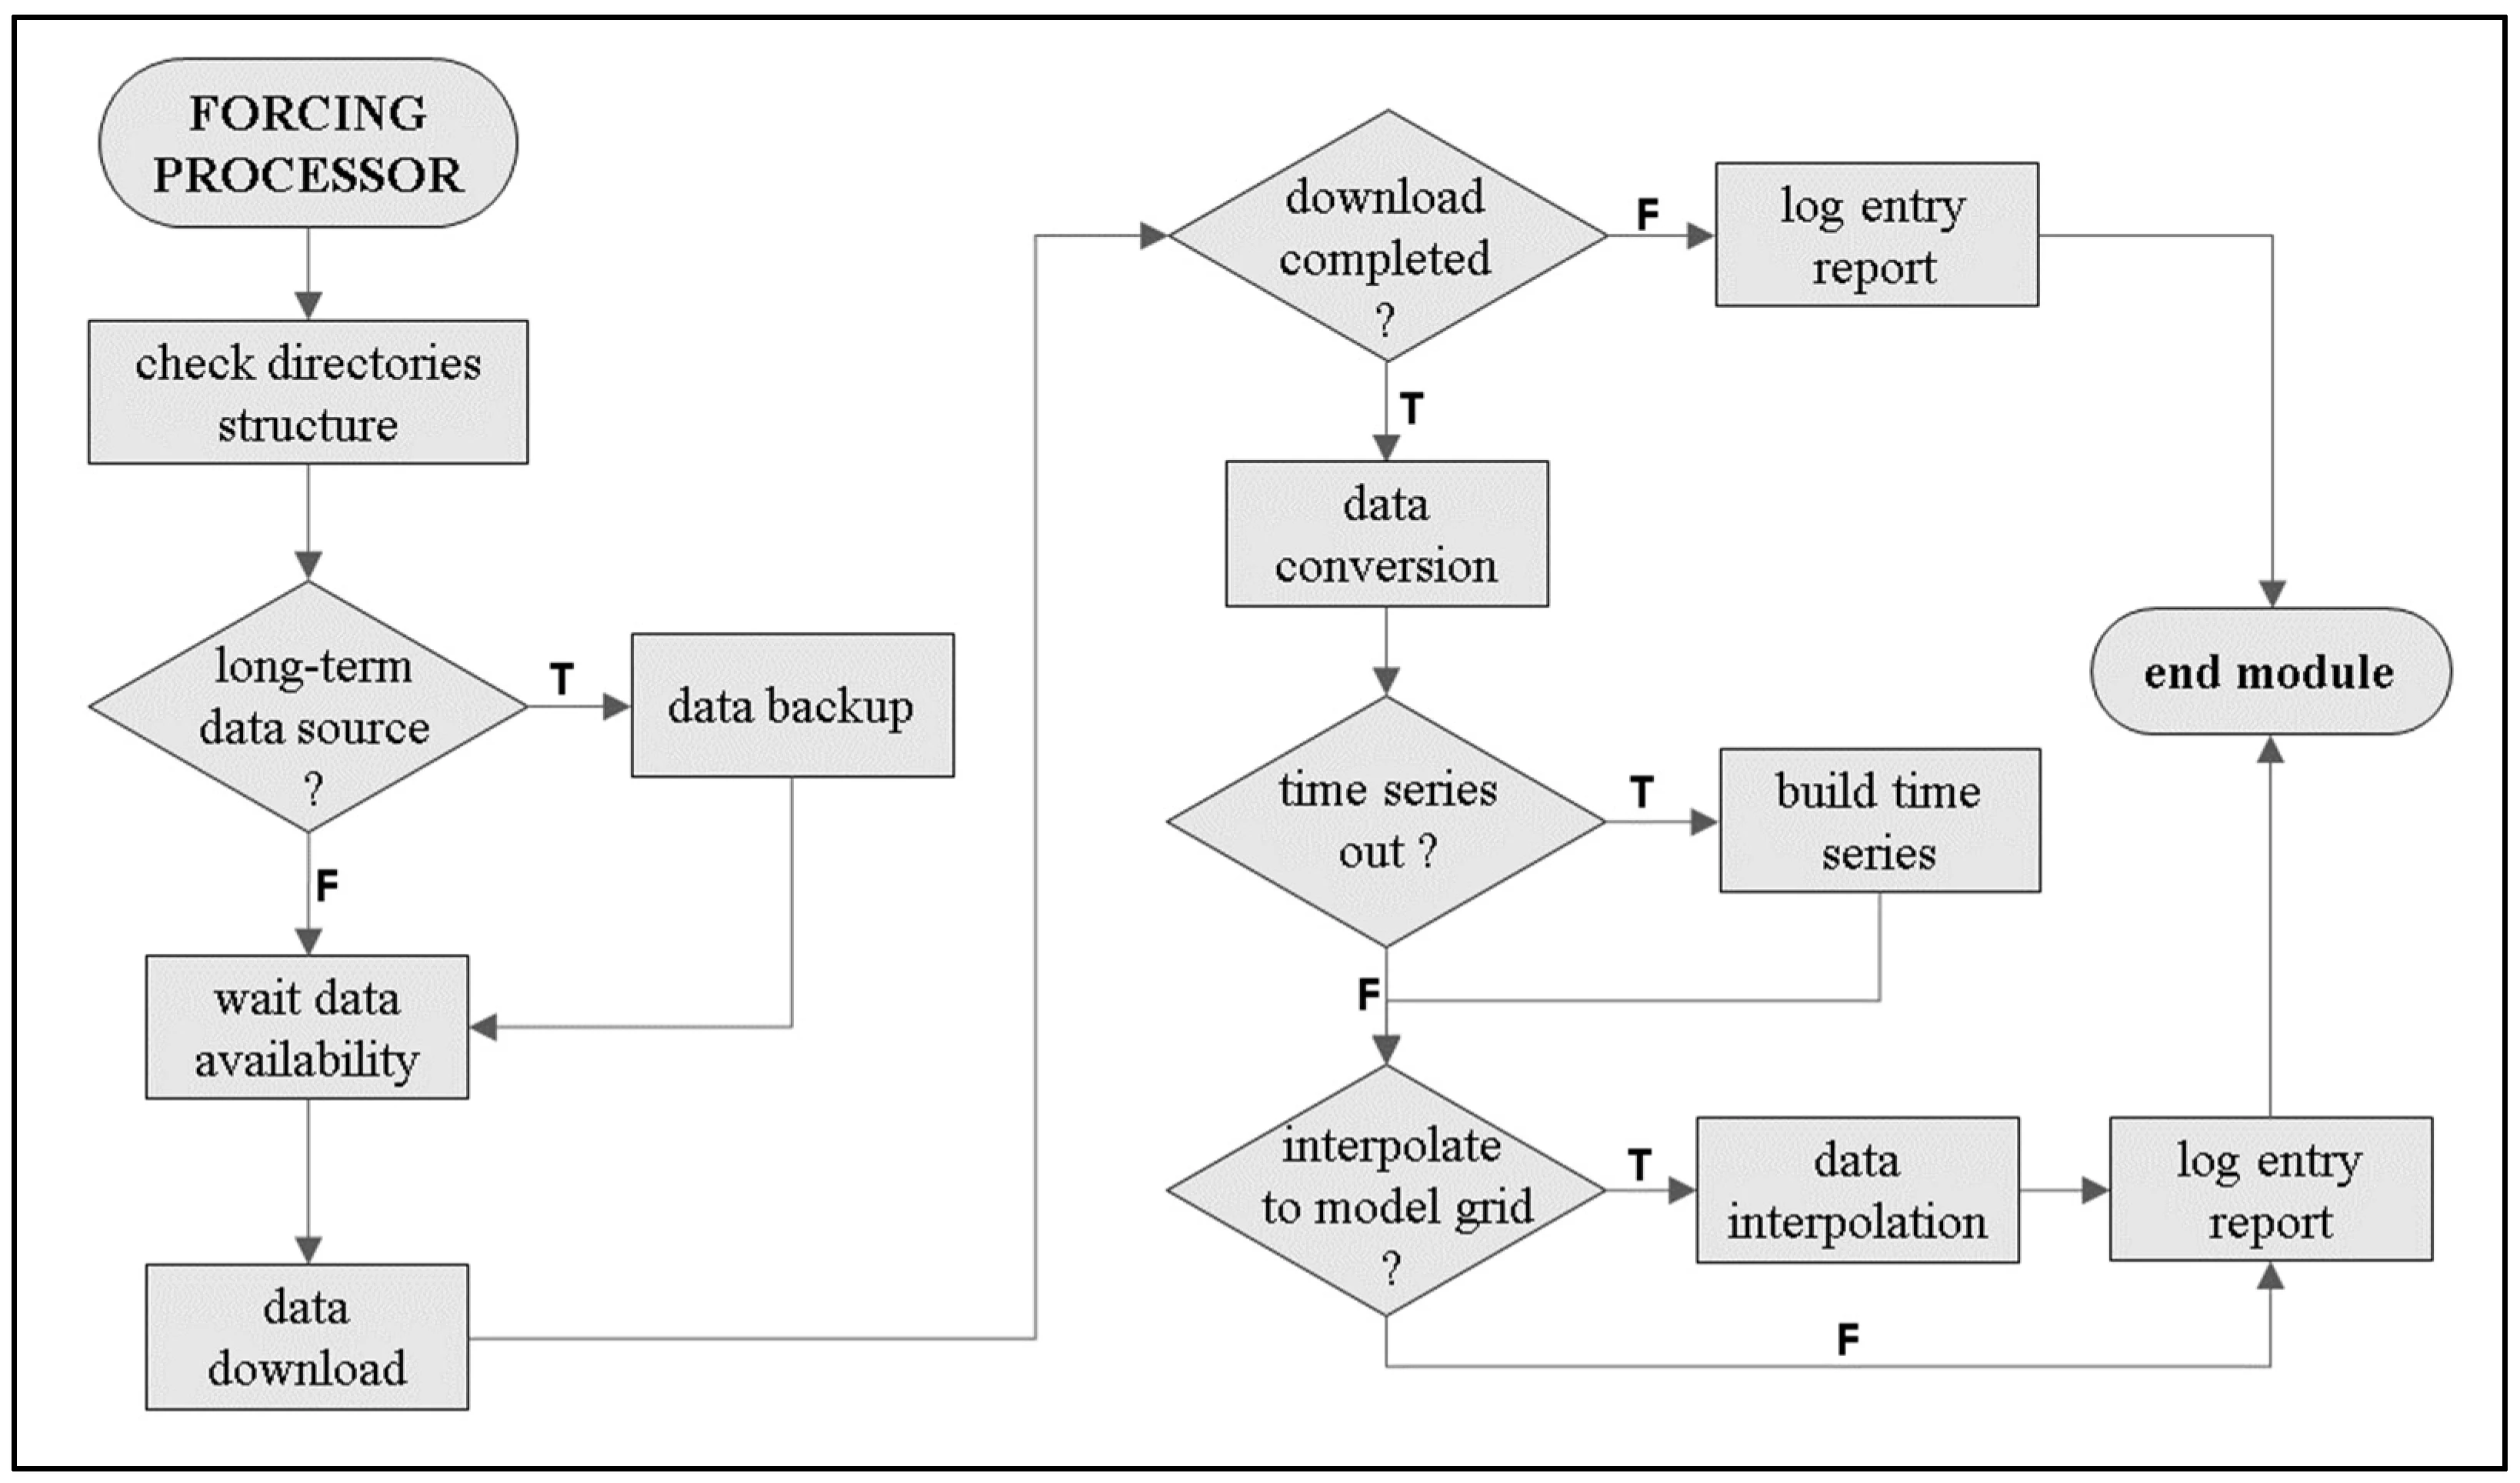
\includegraphics[width=16.0 cm]{figures/fig4.2.png}
    \caption{Generic scheme for SMS-Coastal Forcing Processor, in which the basic operations and sequence are the same for any data provider. The answers for a decision block in all figures with structure charts are given by the characters "T" for true and "F" for false.}
    \label{fig:4.2_forcing}
\end{figure}

Since each supplier has a specific schedule for uploading their data, SMS-Coastal configures the exact start time to trigger the download operation. In this way, SMS-Coastal will pause until the data is available. Additionally, when more than one source must be processed, the programme will queue the download operations, sorted by their start time. Depending on the data provider, the programme can retrieve the files directly from a web page, an FTP repository, or an OPeNDAP server. Other Data Access Protocols can be easily added to the system. If the download fails, the Forcing Processor is terminated for that specific source, and an error report is created. When two or more sources are scheduled for the same start time, the download order corresponds to the order of the inputs in the SMS-Coastal initialization file (see \Cref{subsec:cp4_smsini}).

After the download, SMS-Coastal may convert the data to the format used by the hydrodynamic model being applied, such as from GRIB to NetCDF or from NetCDF to HDF5. If data is needed at just one point of the grid, the tool can be configured to convert it to a time series; otherwise, it can also manage the vertical and horizontal interpolation to the model grid. All files converted and interpolated within the Forcing Processor receive a well-defined name, so that when they are needed in a simulation operation, the Simulation Manager will easily find them. Before ending this component, the code keeps track of the operations for each data source in the created log file and can send an email report to inform on the success or error of the sequence.

\subsection{Simulation Manager} \label{subsec:cp4_simmanager}
SMS-Coastal is designed to handle two types of simulation cycles: one for spin-up simulations, the Restart Run, and another for operational forecasting, the Forecast Run. The Restart Run is used to initialise a model from a certain initial condition or from the data of larger-scale or global solutions. Once the Restart Run is completed, the model is in a more dynamically balanced state, which will serve as a better starting point for the actual forecast simulation.

The diagram in \bCref{fig:4.3_cycles} illustrates the simulation cycle process. The blue ribbons correspond to the Forecast Runs, and each one of them is a three-day forecast simulation. At the end of the simulation of the first day of each Forecast Run, the model writes the initial condition files that will be used the next day. At some point in the week, defined in SMS-Coastal's input file and on day $i + 3$ in the figure, as the initial conditions start to degrade, a Restart Run (yellow ribbon) is executed in hindcast mode to adjust the model internal state to better dynamic conditions. Additionally, as shown in the diagram, both processes are executed simultaneously so that the prediction cycle is not interrupted. This is a representative example; times and durations can be easily adapted to other simulation requirements using the input method of SMS-Coastal (\Cref{subsec:cp4_smsini}).

\begin{figure}[H]
	\centering
    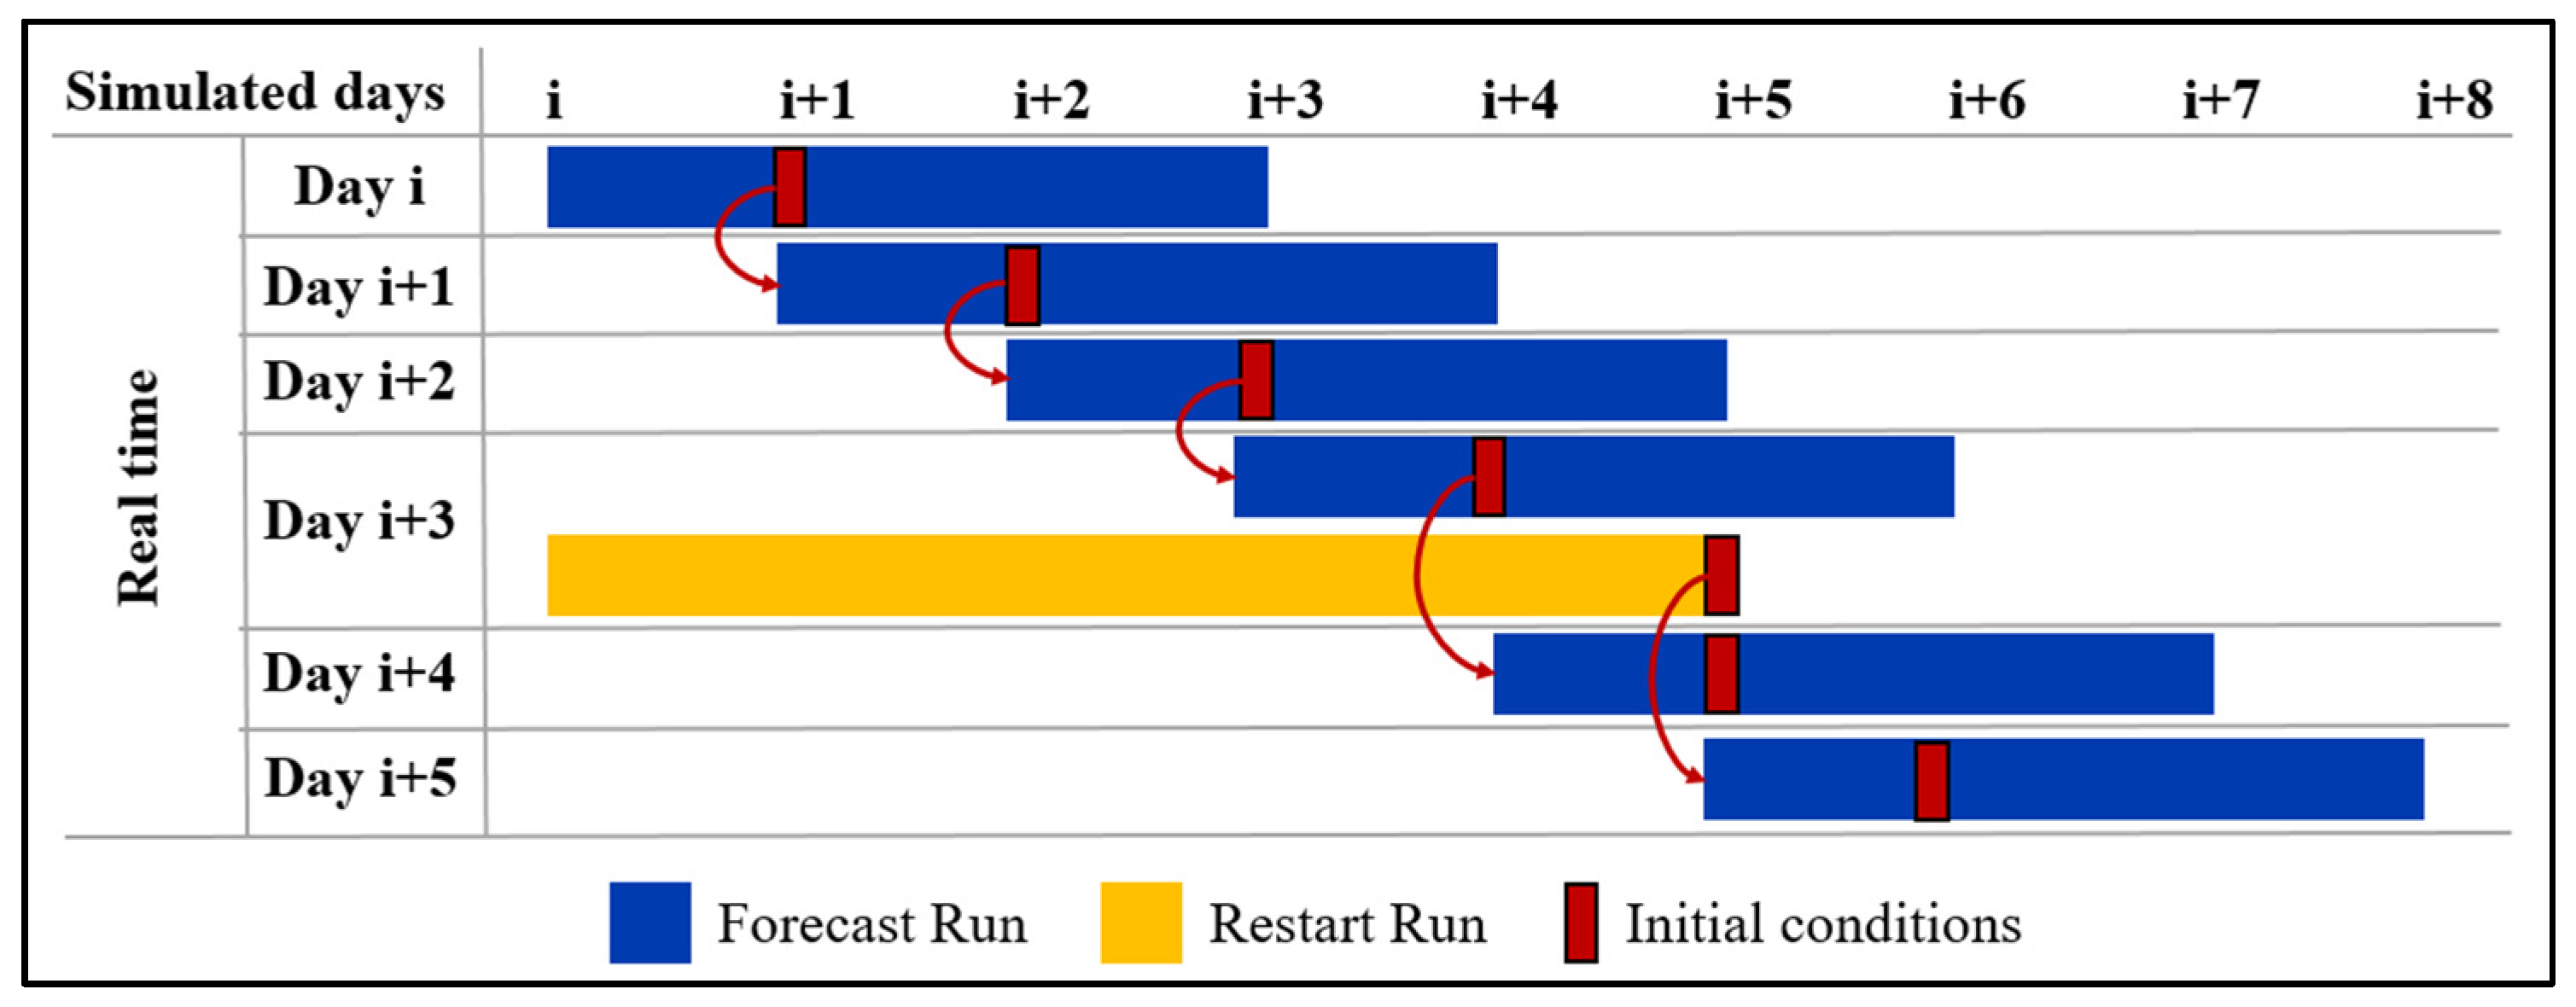
\includegraphics[width=16.0 cm]{figures/fig4.3.png}
    \caption{Forecast and Restart Run processes are being executed by SMS-Coastal. Every day the forecasting process is started, and after one day of simulation time, the initial conditions files for the next day's simulation are generated. Each prediction uses the past simulation files until a Restart Run is performed to produce fresh initial condition files.}
    \label{fig:4.3_cycles}
\end{figure}

\subsubsection{Forecast Run}
The operations sequence conducted in a Forecast Run is summarised in detail in the structure chart in \bCref{fig:4.4_forecast}. Similar to the Forcing Processor, the programme checks the directory structure and prepares the simulation environment by removing all previous run outputs and gathering the essential files. The initial conditions are obtained from the files generated by previous simulation cycles, as explained in item \ref{subsec:cp4_simmanager}. However, whenever a forecast and a spin-up cycle generate initial data for the same date, SMS-Coastal will give preference to those of the Restart Run. This aspect can also be seen in the diagram in \bCref{fig:4.3_cycles}, at day $i + 5$, when the Forecast Run uses the files generated by the Restart Run of day $i + 3$.

\begin{figure}[H]
	\centering
    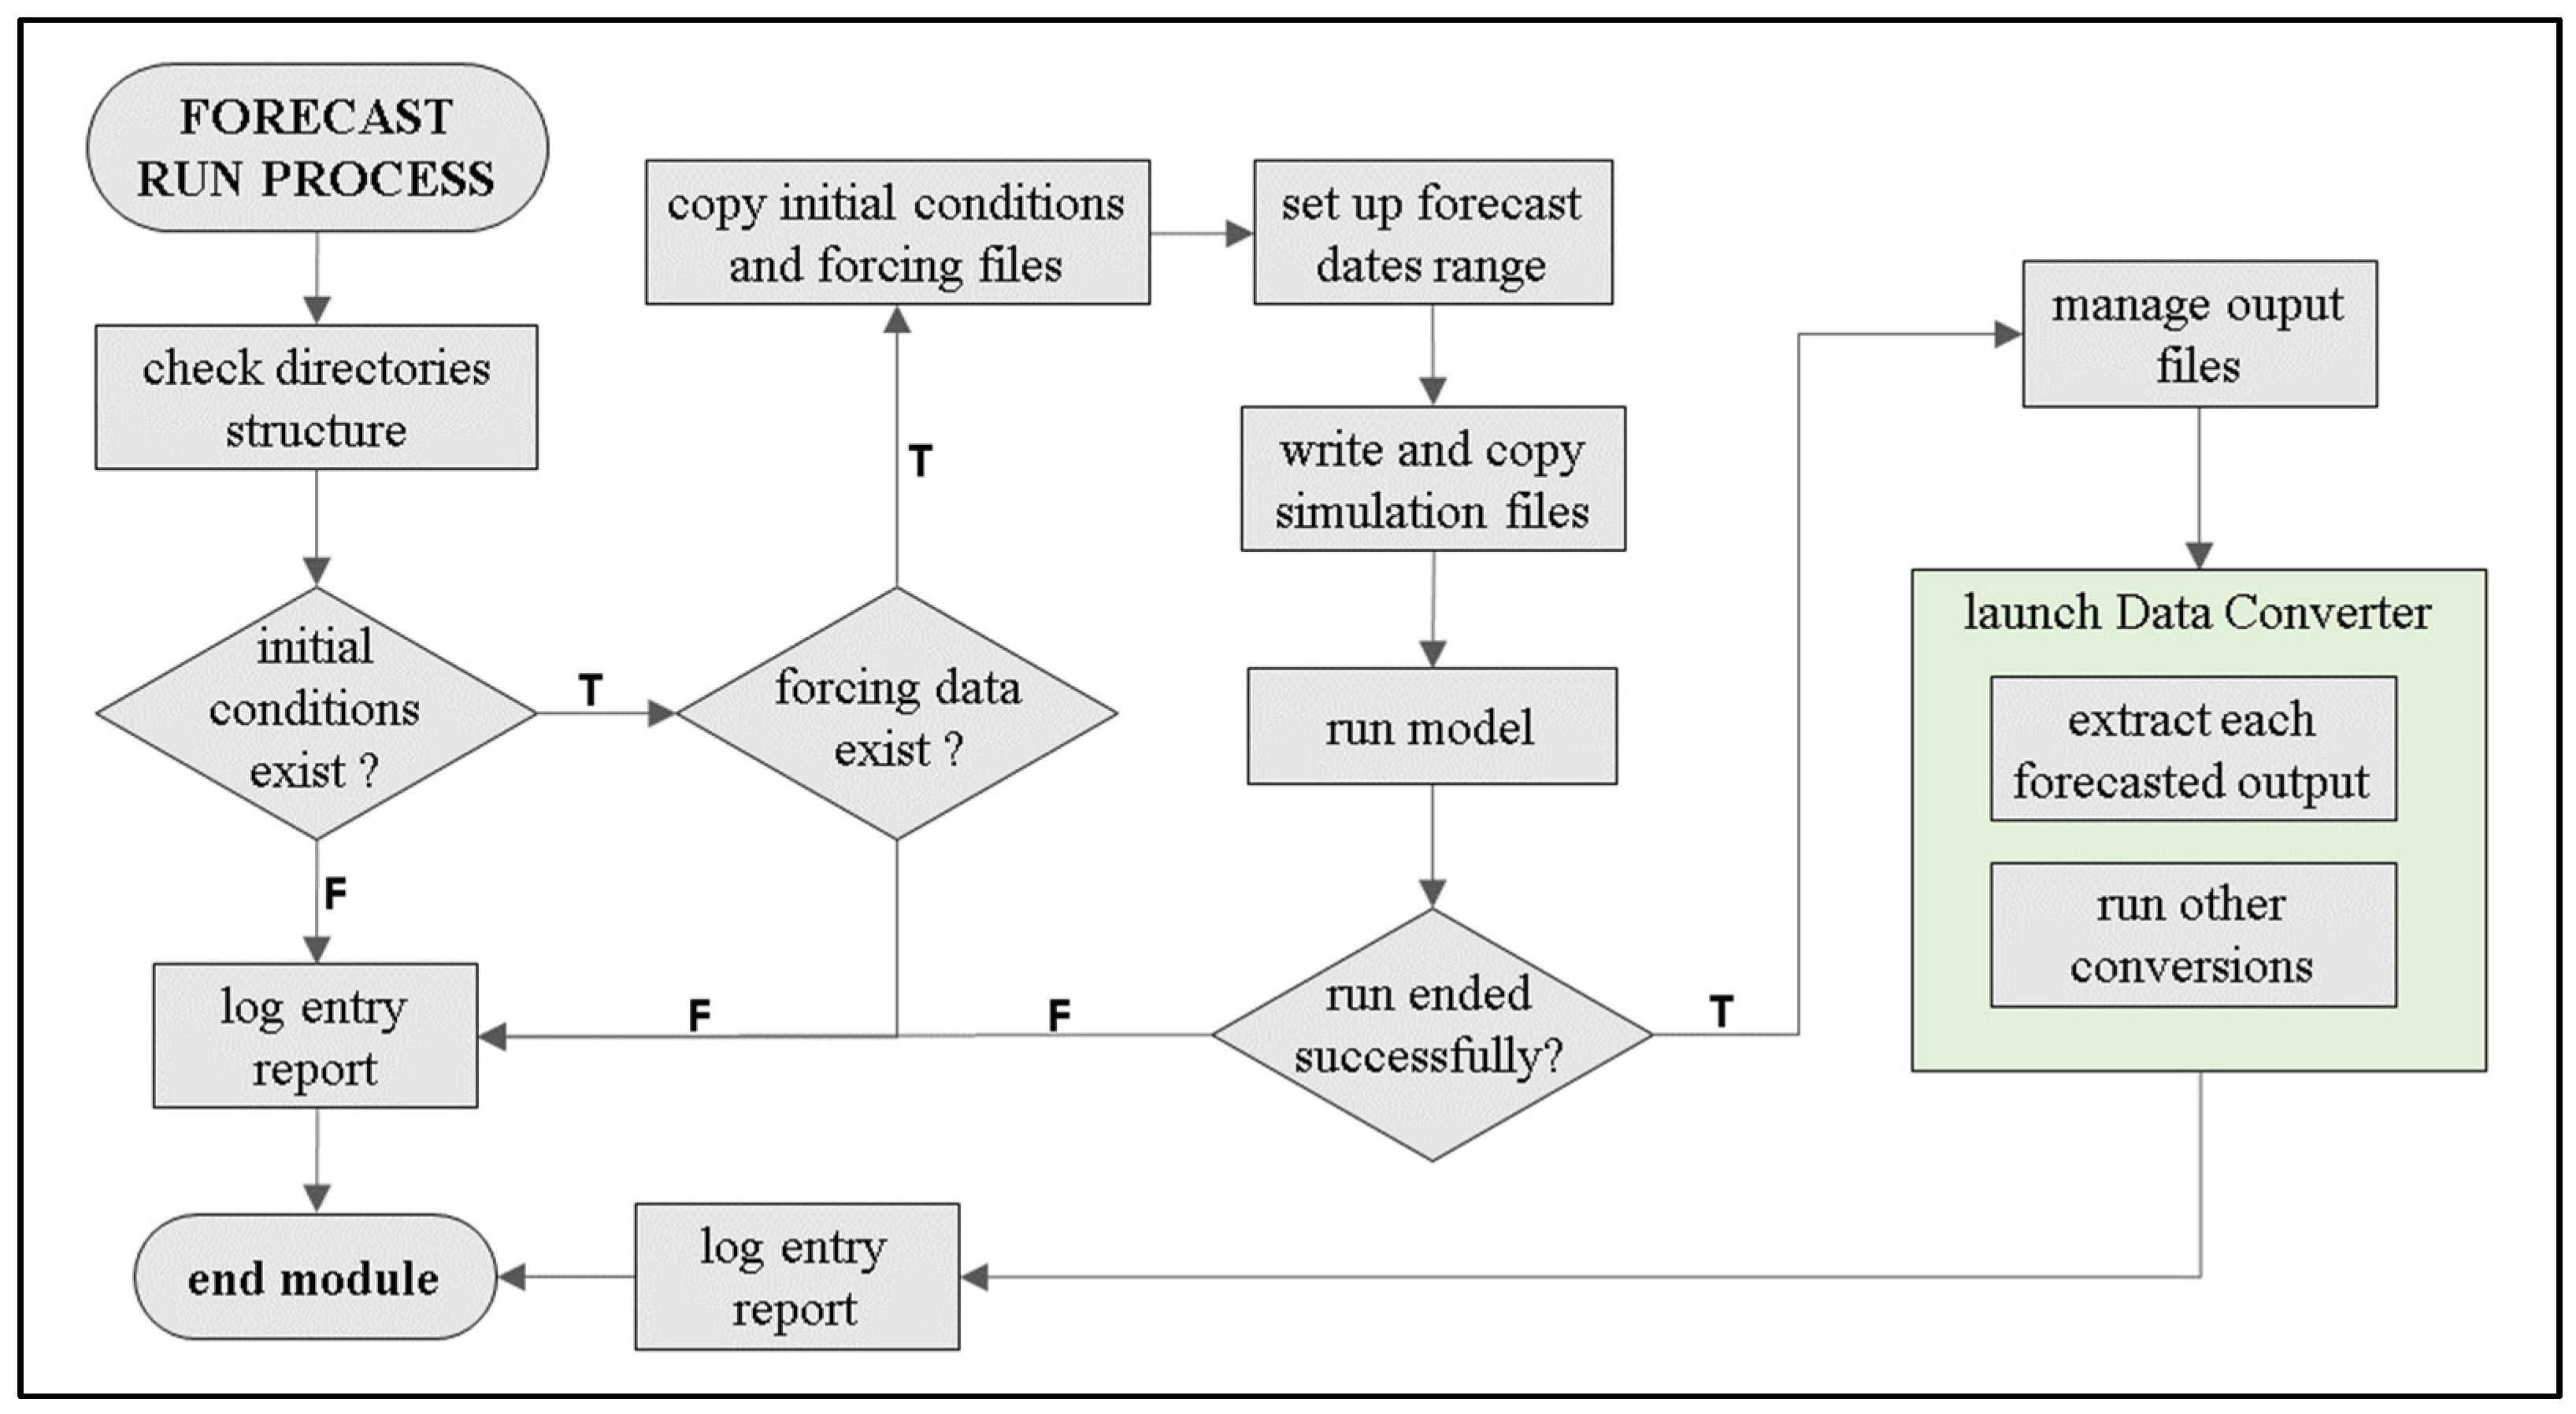
\includegraphics[width=16.0 cm]{figures/fig4.4.png}
    \caption{Forecast Run module's operation sequence. Checking the simulation environment comprises removing data from the previous simulation, creating the necessary folder structure, and preparing the log file. After this, the programme will check the existence of the initial conditions and external forcing data, terminating the module if any data is missing. With the forcing data, it will define the forecast date range to run the hydrodynamic model. If the simulation succeeds, the output files will be saved in a local database, and conversion operations will be launched inside the Data Converter component.}
    \label{fig:4.4_forecast}
\end{figure}

When searching for forcing data, the tool selects the most recent one produced by the Forcing Processor component. In this way, SMS-Coastal keeps the forecast operational and on time, even if that component fails to obtain newer data. Furthermore, it makes an adjustment of the forecast range to the maximum possible by comparing the time outputs of the selected forcing data with the range defined in the programme inputs.

After the data setup, SMS-Coastal copies and writes the model configuration files, initiates the hydrodynamic model executable, and waits until its completion. If the forecast simulation fails, it writes the error record in the log file and exits the module. If it succeeds, all output files are copied to a local database. By default, the Data Converter component is launched to prepare files for archiving in an external database and for use in conversion operations. However, as the components are independent from each other, this feature can be disabled. At the end, the code writes a success message in the log and ends the module.

\subsubsection{Restart Run}
This step is described from the perspective of a model spin-up. An alternative to this could be the analysis cycle of a data assimilation scheme. Essentially, the result will be the same: to provide fresh initial conditions for the next forecast cycle. This methodology is very common in coastal and local models when there is a reliable global base solution in the background. The spin-up process follows a methodology very similar to that described in \textcite{leitao2005modelling}.

The sequence of operations performed in the Restart Runs shares some similarities with the Forecast Runs, as shown by the structure chart in \bCref{fig:4.5_restart}. There are, however, two major differences: the first is that there is no need to search for initial conditions files from a previous simulation since the model initiates from external initial and boundary conditions. The second is that the runs can be performed in stages with a gradual increase in time to prevent simulation instability. Due to this, SMS-Coastal does a repetition cycle to run each of the stages as shown in the figure, from stage 1 to \emph{n} $(n \in \mathbb{N}, n > 0)$.

Considering the extensive duration of restart simulations, which encompass a hindcast spanning several days (refer to \bCref{fig:4.3_cycles}), and that that is performed with gradual step time, it is important to acknowledge that the execution of all stages may exceed a single day in real time. In such cases, the generation of initial condition files for the last stage could experience a delay that renders them unusable for the Forecast Run of that particular day. To address this issue, SMS-Coastal incorporates an additional simulation stage to cover the period between the completion of the previous stage and the subsequent forecast, ensuring the provision of suitable initial conditions for the following Forecast Run. This aspect can also be seen in the diagram in \bCref{fig:4.3_cycles}, where the Restart Run on day $i + 3$ did not generate initial conditions for the forecast of day $i + 4$, but for day $i + 5$.

\begin{figure}[H]
	\centering
    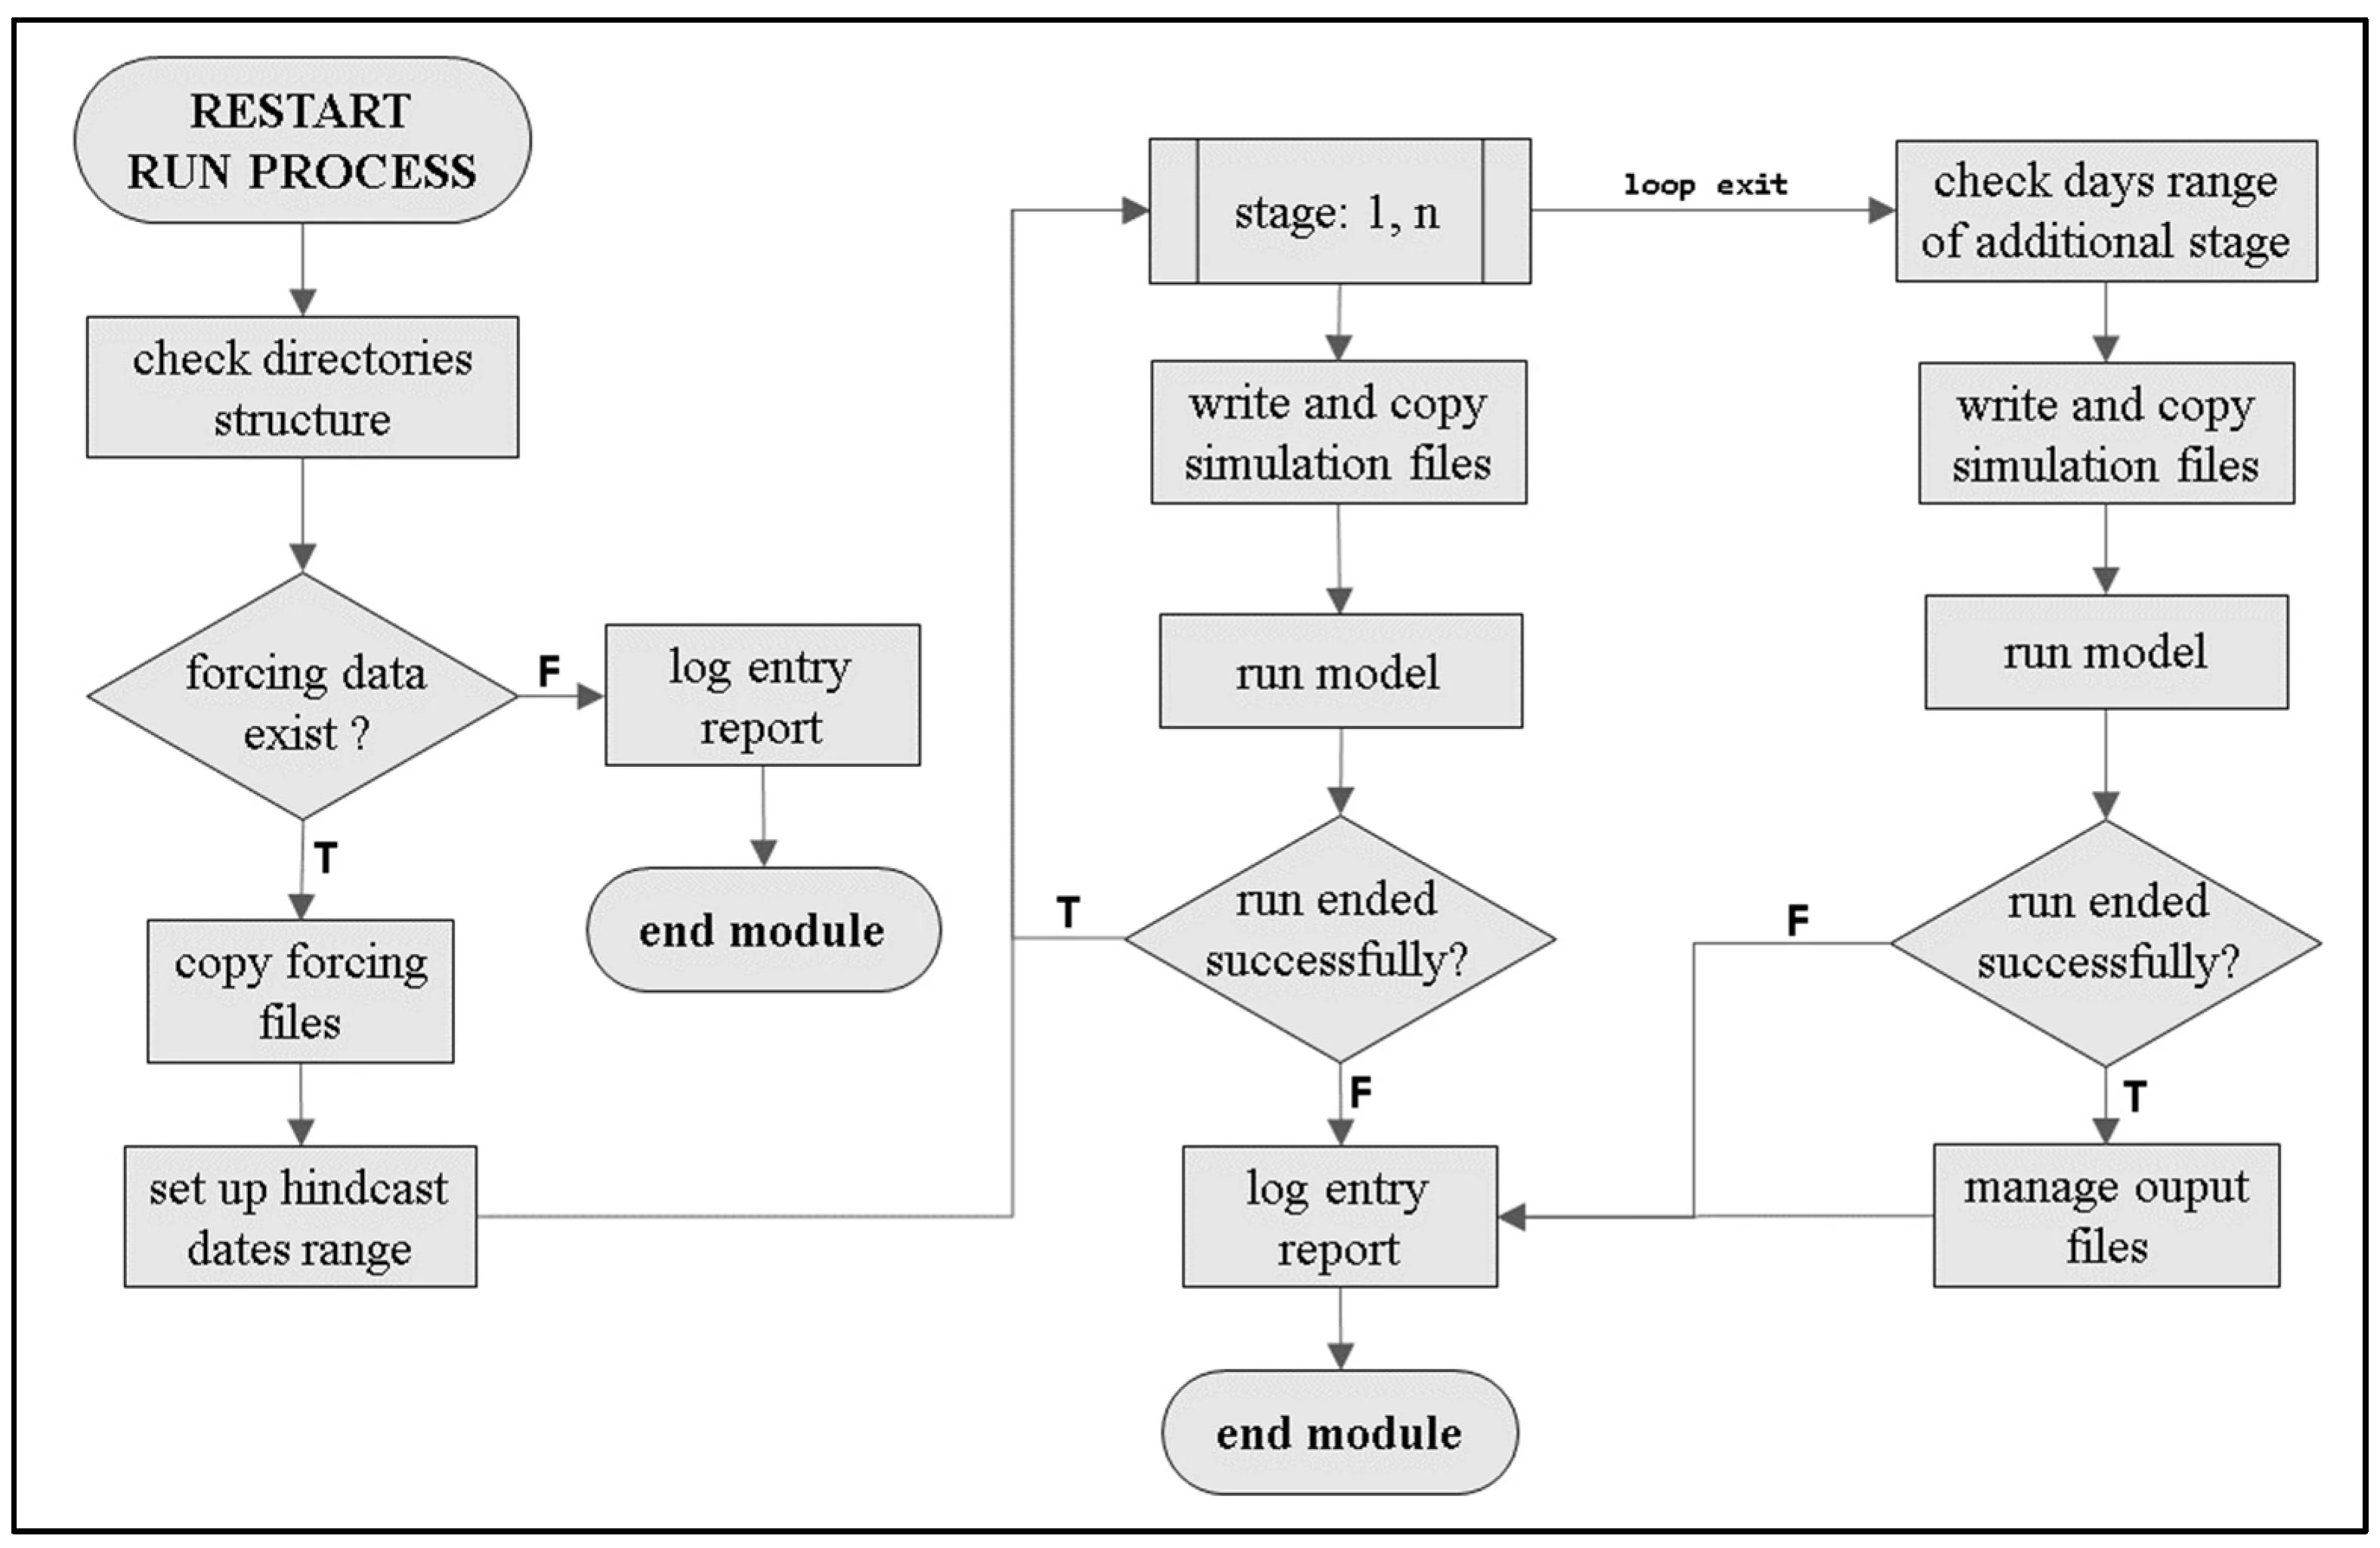
\includegraphics[width=16.0 cm]{figures/fig4.5.png}
    \caption{Restart Run module's operation sequence. The environment is set up in the same way as in a forecast, as is its time range. However, it does not need initial data from a previous simulation, and the restart can consist of more than one simulation or be conducted in stages that are conducted in a loop. After the final stage, an additional simulation is performed to generate initial condition files for the next Forecast Run.}
    \label{fig:4.5_restart}
\end{figure}

\subsubsection{Runs Manager}
Considering that the forecast and spin-up processes are executed simultaneously, it was necessary to create the Runs Manager, the structure within the Simulation Manager that controls the Forecast and Restart Runs. It starts by running an instance of the Forcing Processor with the simulation dates as inputs to generate new forcing data. It then spawns a subprocess for the Forecast Run and another for the Restart Run. The latter, however, will only be executed on the day determined by the programme's inputs, e.g., once a week. The cycles must run in separate parallel subprocesses so that the prediction cycle will not be interrupted.

\subsection{Initialization File} \label{subsec:cp4_smsini}
SMS-Coastal was mainly designed to automate all the operations involved in producing coastal models' daily forecasts. For this reason, the Simulation Manager can also run instances of the Forcing Processor and Data Converter components. However, since they are independent of each other, the programme's initialization file can be configured to select specific functions and use SMS-Coastal for other purposes, e.g., process forcing data with the Simulation Manager disabled; run a simulation operation with the Forcing Processor disabled, making the Simulation Manager fetch previously processed data.

The initialization file is a text file that receives all user inputs to configure how and what SMS-Coastal should do. The programme's first operation is to read this file and check all inputs, which are a series of instructions organised in a similar system to Python dictionaries. In fact, the programme code converts these inputs into a dictionary, making the order of the entries irrelevant. Each file line has a keyword representing one SMS-Coastal execution variable and its value, which can be of any type (integer, float, or list) according to the key. Therefore, the execution variables supply information about which operation to run, the simulation date range, a list of oceanic and atmospheric external data sources, the number of model levels, when to perform the Restart Run, a list of e-mail addresses to send the reports to, what conversion operations to run, and other information. Examples of the input method for SMS-Coastal can be found on its GitHub page (see \Cref{sec:cp4_github}).

\section{Results} \label{sec:cp4_results}
The performance of SMS-Coastal is presented in this section using two different realisations of operational models using MOHID. Regardless, the tool can be upgraded to handle any other operational system. MOHID is a modelling system designed to model the marine environment with a modular architecture, programmed in ANSI FORTRAN, and features to simulate physical, chemical, and biological processes of the marine environment \parencite{neves2007numerical, braunschweig2004object, sobrinho2021improving, garneau2017modelling}. The two operational models used for testing SMS-Coastal are the Algarve Operational Modelling and Monitoring System (SOMA), a high-resolution operational model for the Portugal south coast, and BASIC, the 3D operational model of the Cartagena Bay in Colombia. The associated operational systems have been operating for almost four years in SOMA's case and a little over three years in BASIC's.

SOMA is a 3D system that encompasses two increasing resolution levels: one with 2 km grid cells and another with 1 km grid cells. The details regarding the model's implementation can be found in \textcite{janeiro2017integrating}. It produces four-day forecasts of currents, salinity, and temperature and has been operational since 7 July 2019. Designed in a much smaller area, BASIC is a single resolution-level 3D model with 75 m grid cells, whose implementation details are in \textcite{tosic2019hydrodynamic}. It generates three-day forecasts of currents, salinity, and temperature and has been operational since 1 May 2020. Each model runs in a virtual machine on the same server, sharing the same Intel(R) Xeon(R) Gold 6138 processor with a base frequency of 2.00 GHz. However, the resources allocated to each are not the same. SOMA has 10 virtual processors, 9.76 GB of RAM, and 450 GB of data space, while BASIC has 6 virtual processors, 8.00 GB of RAM, and 200 GB of data space.

Considering that SMS-Coastal was built to manage any MOHID-based operational system, it was necessary to develop a generic directory structure so that they could work together. In this case, the structure was mirrored for the two managed systems. The general structure is represented by the scheme in \bCref{fig:4.6_dirtree}. The folder and file names are fixed inside this structure for standardisation reasons. The contents of each simulation folder are as follows:

\begin{itemize}
    \item \emph{FORC}: folder used by the Forcing Processor to download, process, and store oceanic and atmospheric external forcing data.
	\item \emph{Hydrodynamic Model}: contains the executable of the hydrodynamic model in use and all its necessary libraries and dependencies.
	\item \emph{Forecast}: folder to be used by Forecast Run processes.
	\item \emph{Restart}: folder to be used by Restart Run processes.
	\item \emph{SMS-Coastal.py}: representation of all SMS-Coastal Python modules.
	\item \emph{init.dat}: SMS-Coastal initialization file with all user inputs.
\end{itemize}

For each simulation type, there is a folder with the same internal structure, containing \emph{General Data}, \emph{Operations}, and the model's first-level folder. The first one is used by SMS-Coastal to store common input files between all levels, such as bathymetry data files, initial and boundary conditions, time series locations, tide information, and processed oceanic and atmospheric operational data. The programme will use the \emph{Operations} folder to build the model's local database by placing in it all simulation outputs and log files, as well as formatted and converted results, as well as files in case of a failed run.

The folder structure demonstrated in \bCref{fig:4.6_dirtree} fits an n-level nested project. Each level has three folders to store its respective input and output files: \emph{data} for the set of data files with the user-defined parameters for the resolution of the hydrodynamic model governing equations; \emph{exe} for the files related to the simulation execution, which is also the domain working directory; and \emph{res} for all the domain's current simulation outputs. When applicable, it will have one more folder for the subsequent level. Part of this entire folder structure does not need to be previously defined, as SMS-Coastal, when executed, checks and creates all the missing structures, as is the case for the folders \emph{FORC}, \emph{Operations}, \emph{exe}, and \emph{res} of each level.

\begin{figure}[H]
	\centering
    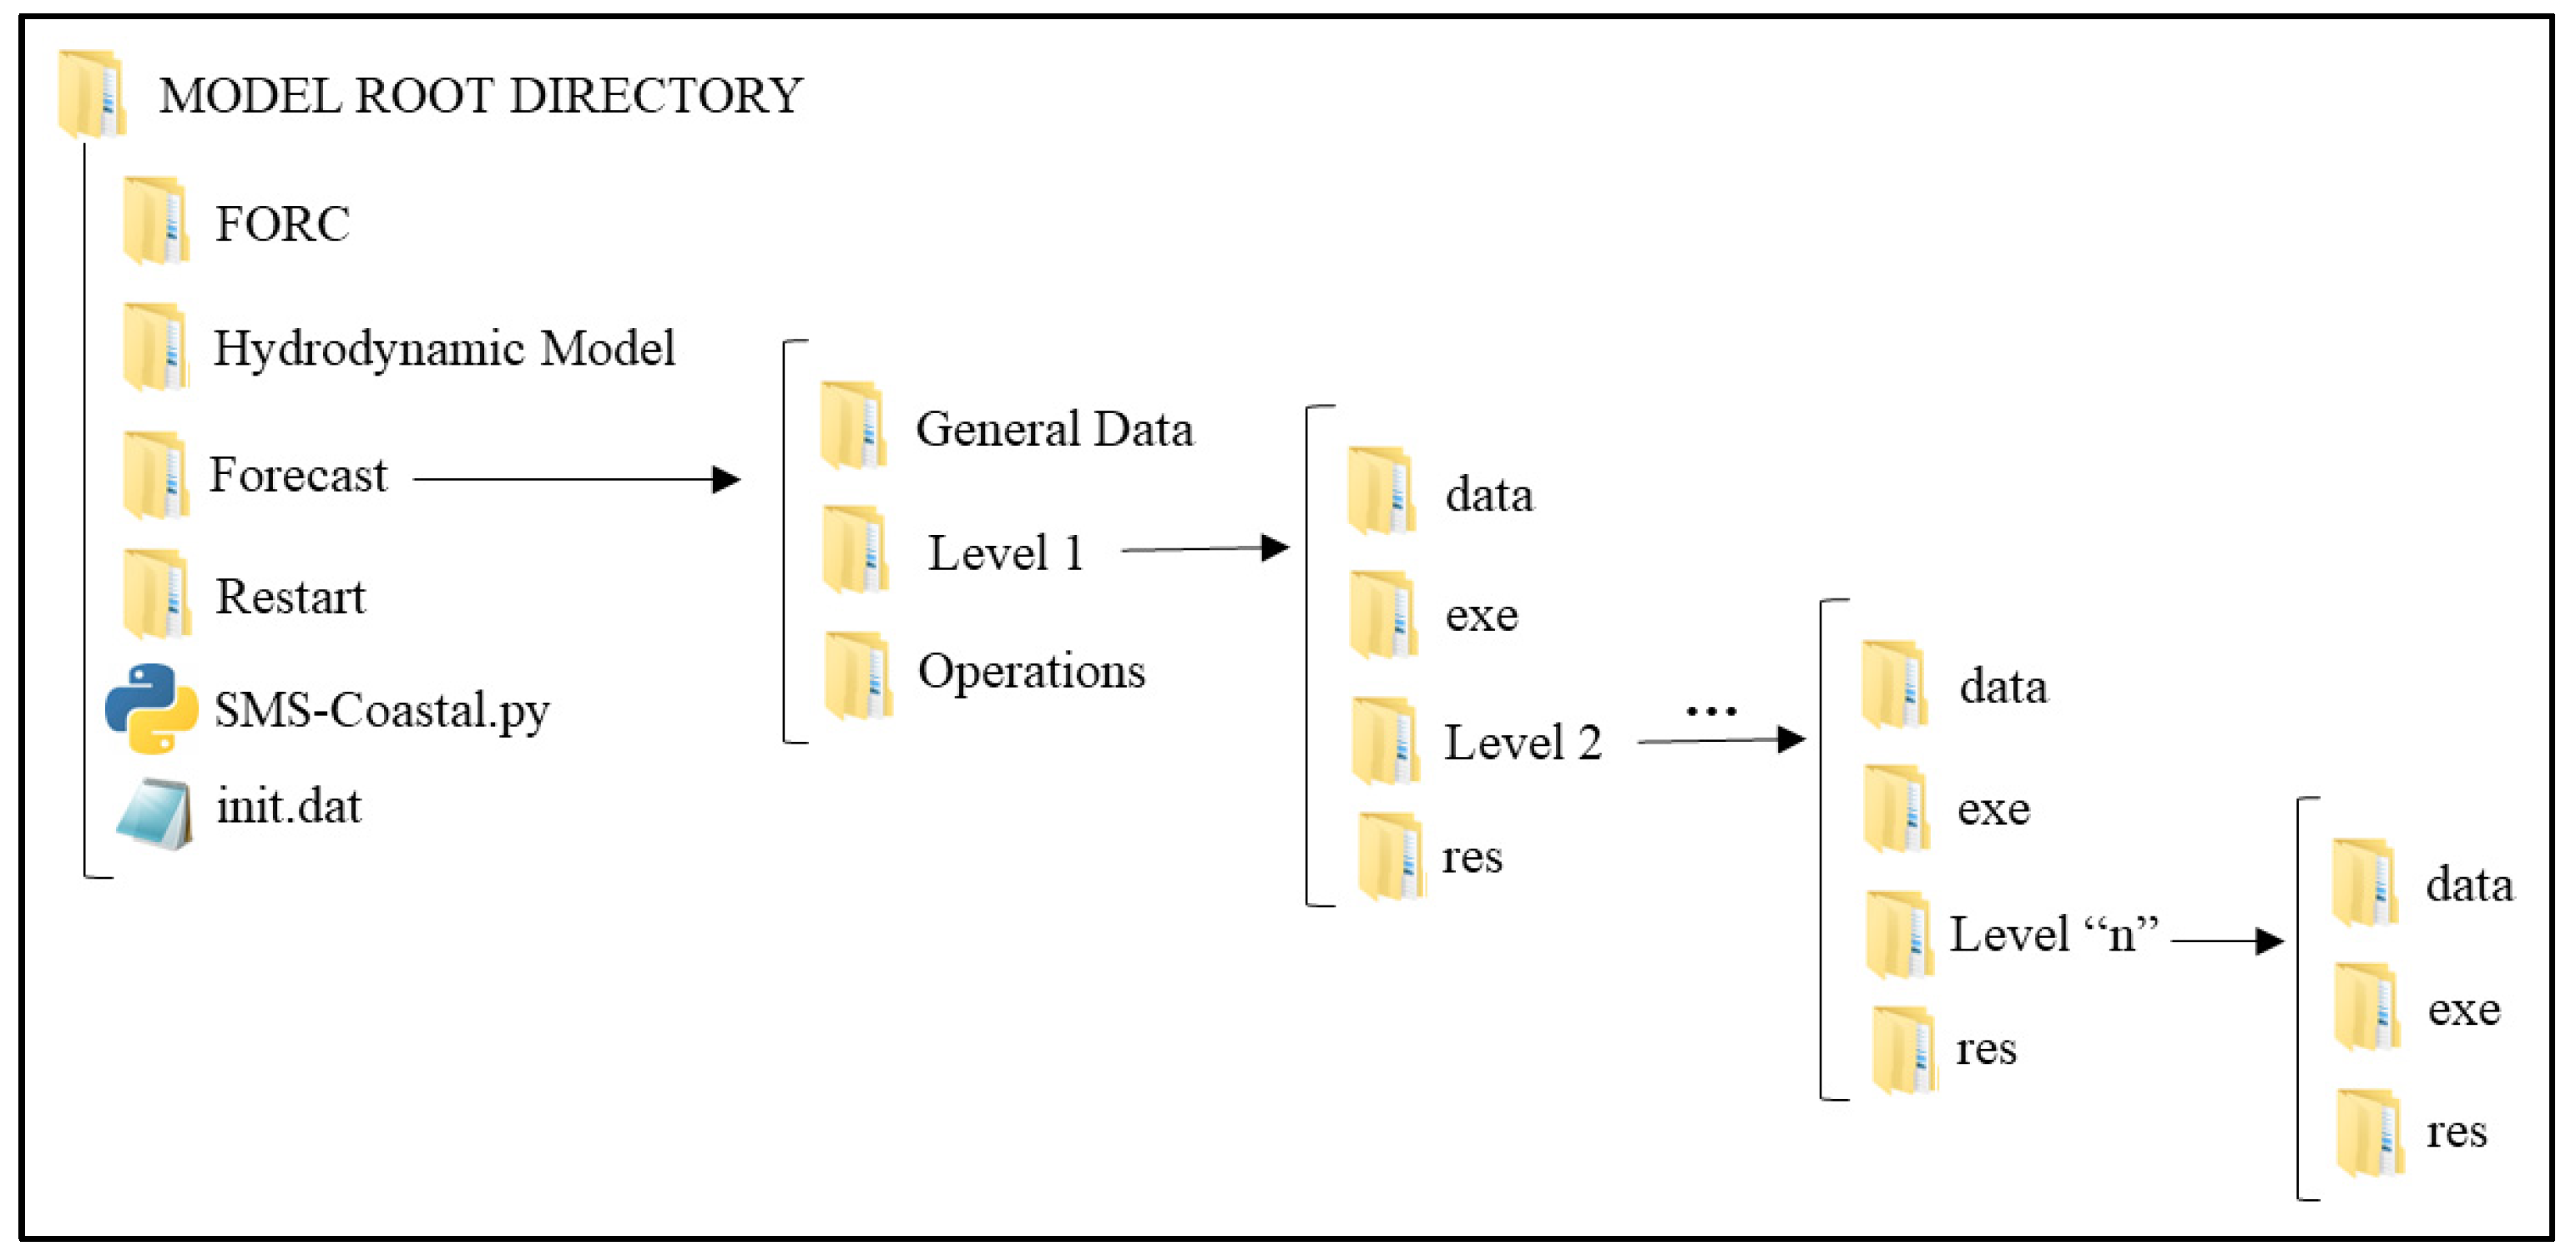
\includegraphics[width=16.0 cm]{figures/fig4.6.png}
    \caption{Schematic of the generic folder structure to be used by SMS-Coastal to manage an n-levels model. The root directory contains a folder for the Forcing Processor component operations, one for the hydrodynamic model files, and one for each simulation type, Restart Run and Forecast Run. The structure of the simulation folders is identical: \emph{General Data} to store common input files for all levels; \emph{Operations} as a local database for simulation output files; and one folder for each level of the model to store current simulation input and output files.}
    \label{fig:4.6_dirtree}
\end{figure}

Based on the log files of the SOMA and SMS-Coastal integrations, until the end of June 2023, over 1500 simulations were executed, of which 1518 were Forecast Runs and 234 were Restart Runs. On the other side, BASIC and SMS-Coastal integration accounted for 1351 runs, with 1211 Forecast Runs and 140 Restart Runs, until the same end date. Inevitably, not all runs were successful, considering that data providers, models, servers, and SMS-Coastal are susceptible to failure. \bCref{tab:4.1_failures} contains the failure statistics, that is, the simulations that did not finish successfully, for each model during this lifespan. \bCref{fig:4.7_failures} depicts the graphical representation distributed in time of the stops presented in \bCref{tab:4.1_failures}. In the table, the stops were classified into those caused by internal and external factors, including the following events:

\begin{itemize}
    \item \emph{Code error}: SMS-Coastal code optimisation is needed.
	\item \emph{Initial condition missing}: SMS-Coastal was unable to find proper initial condition files from previous Forecasts or Restart Runs.
	\item \emph{Insufficient virtual memory}: the simulation aborted due to a lack of space in computer random-access memory (RAM).
	\item \emph{Model error}: simulation aborted by the hydrodynamic model.
	\item \emph{Server error}: the virtual environment crashed.
	\item \emph{Forcing files missing}: SMS-Coastal was unable to find suitable forcing files from providers.
\end{itemize}

In order to ensure the proper functioning of SMS-Coastal's generic code during simulation management, it is crucial to adhere to the prescribed structure of files and folders. Thus, to initiate a simulation operation, the model must be arranged as depicted in the root directory illustrated in \bCref{fig:4.6_dirtree}. The parameters of the equations should be stored within each respective \emph{data} folder at their respective levels. Additionally, the necessary inputs must be appropriately specified in the initialization file named \emph{init.dat}. Once these steps are completed, the SMS-Coastal application can be executed. It is of utmost importance to accurately configure the input file, as the programme verifies all keywords and halts execution if any discrepancies are detected. However, in the context of executing continuous forecast cycles, the \emph{init.dat} file only requires configuration once, ensuring subsequent operations can proceed smoothly.

\vspace{20mm}

\begin{table}[H]
	\centering
	\caption{Failures observed for the models during the simulation management conducted by SMS-Coastal. The values for the Algarve coast model (SOMA) correspond to 1752 runs performed between July 2019 and June 2023, and for the Cartagena Bay model (BASIC), 1351 runs between May 2020 and June 2023.}
	\label{tab:4.1_failures}
    \footnotesize
	\begin{tabularx}{\textwidth}{
        >{\raggedright\arraybackslash}m{32mm}
        >{\raggedright\arraybackslash}m{18mm}
        >{\centering\arraybackslash}m{11mm}
        >{\centering\arraybackslash}m{13mm}
        >{\centering\arraybackslash}m{13mm}
        >{\centering\arraybackslash}m{11mm}
        >{\centering\arraybackslash}m{13mm}
        >{\centering\arraybackslash}m{13mm}
        }
		\toprule
		& & \multicolumn{3}{c}{\textbf{SOMA}} & \multicolumn{3}{c}{\textbf{BASIC}}\\
		\midrule
		\textbf{Stop Type} & \textbf{Stop Class} & \textbf{Stops} & \textbf{\shortstack{\% of\\Stops}} & \textbf{\shortstack{\% of\\Runs}} & \textbf{Stops} & \textbf{\shortstack{\% of\\Stops}} & \textbf{\shortstack{\% of\\Runs}}\\
		\midrule
        Code error                  & internal & 25 & 19.4\% & 1.4\% & 6  &  7.5\% & 0.4\% \\
		Missing initial conditions  & internal & 22 & 17.0\% & 1.3\% & 38 & 47.5\% & 2.8\% \\
		Insufficient virtual memory & internal & 9  &  7.0\% & 0.5\% & -  & -      & -     \\
		Model error                 & internal & 30 & 23.3\% & 1.7\% & 2  & 2.5\%  & 0.1\% \\
		Server error                & internal & 7  &  5.4\% & 0.4\% & 5  & 6.2\%  & 0.4\% \\
		Forcing files missing       & external & 36 & 27.9\% & 2.1\% & 29 & 36.3\% & 2.1\% \\
		\midrule
		Total & & 129 & 100\% & 7.4\% & 80 & 100\% & 5.8\%\\
		\bottomrule
	\end{tabularx}
\end{table}

\vspace{\fill}

\begin{figure}[H]
	\centering
    \includegraphics[width=16.0 cm]{figures/fig4.7.png}
    \caption{Failures over time for SOMA (\textbf{A}) and BASIC (\textbf{B}). As can be seen in B, since BASIC was launched only in May 2020, there are no stops computed for the time before that. No pattern of failure could be observed for the models. However, it was expected to have more stops at the beginning of each operational sequence since the SMS-Coastal generic code was being put to the test while managing the models.}
    \label{fig:4.7_failures}
\end{figure}

\section{Discussion} \label{sec:cp4_discuss}
SMS-Coastal, a software designed to oversee operational cycles of coastal and oceanic models, was employed in this study to effectively manage forecast simulations for two MOHID-based systems. Over time, since the initial release of the programme, significant enhancements have been implemented in its source code, accompanied by the addition and removal of various modules.

One significant challenge of continuous simulation cycles is the limited availability of local storage space to accommodate the extensive volume of generated outputs. Within just a few days of execution, an enormous amount of data can accumulate. In the case of SOMA, which encompasses two downscaling levels, a four-day forecast alone consumes approximately 8 GB of disc space. Given this aspect, it becomes crucial to devise an efficient data management strategy. As a result, several SMS-Coastal processes adopt the practise of overwriting outdated simulation files and integrating modules within the Data Converter to facilitate the transfer of the model's local database to an external storage system. This approach helps reduce storage constraints and ensures the continuation of operational simulations.

As exposed in \bCref{subsec:cp4_simmanager}, a simulation operation will split SMS-Coastal execution into more than one process. This is the case with a Restart Run, which must start in parallel with the Forecast Run. Therefore, as the runs are concomitantly handled by the multiprocessing Python built-in module, they are placed in separate folders inside the project directory (\bCref{fig:4.6_dirtree}). Furthermore, in our specific computer configuration, we observed a reduction in Forecast and Restart Run performances when both were running at the same time. Nevertheless, SMS-Coastal automatically monitors the end events of both processes to continue execution.

SMS-Coastal has maintained SOMA in operational mode since the beginning of July 2019. According to \bCref{tab:4.1_failures}, the model was unable to complete 129 runs, which represents less than 8\% of the total number of runs. Until November 2019, the larger number of internal failures, as shown by the (A) plot of \bCref{fig:4.7_failures}, resulted from problems in the programme's code that accounted in total for less than 20\% of stops. This kind of interruption is always expected at the beginning of the implementation of SMS-Coastal into a new model. However, they can be viewed with optimism and used to improve the system by making it more robust and generic. The stops related to insufficient virtual memory are a specific cause of the model error stops, which were separately counted as they represent a situation that is related to SMS-Coastal. Newer versions of the management system were able to eradicate that problem.

BASIC has benefited from a more consolidated version of SMS-Coastal since, when its operational forecasting started, SMS-Coastal had already been used with SOMA for 10 months. For this reason, fewer code adjustments were necessary, and, as seen in \bCref{tab:4.1_failures}, interruptions caused by programming problems represented less than 1\% of total runs. The Cartagena Bay model had 1351 runs and was interrupted 80 times, or less than 6\% of total runs. During this period, however, the model did not run for 10 days between October and November 2020 due to the suspension of the atmospheric data provider. BASIC has proved to be quite reliable since it has registered only two failures caused by numerical instabilities in the model. The significant increase in failures in December 2022 was due to the introduction of a new version of the code, which had some errors corrected as it was performing simulation cycles.

One major source of error in both models was the lack of external forcing data, caused mainly by the unavailability of the downloads. SMS-Coastal still has no other option but to abort a simulation if the required external data is missing, but future versions can be upgraded to retry the download after a waiting time. In \bCref{tab:4.1_failures}, this class of stops was classified as an external factor; more than a quarter of all stops in SOMA runs were due to this factor, and in BASIC, the number is even higher, just over 36\%. In the last model, several sequential stops of this type caused stops in the following days due to missing initial condition files. Together, they accounted for more than 80\% of the total stops in BASIC. This fact is evident in the (B) plot of \bCref{fig:4.7_failures}, for the months of May and October 2020.

\section{Conclusions} \label{sec:cp4_conclusion}
This research introduces SMS-Coastal, a self-contained software that implements a generic framework for managing forecast simulations in MOHID-based operational coastal models. Simulation management encompasses coordinating diverse operations and file handling. To enable users to specify operation parameters for each specific system, the software adopts a method of reading keywords from an initialization file. Consequently, SMS-Coastal serves as a versatile tool for managing operational coastal and oceanic models, which is a critical step in supporting the Blue Economy.

The software was developed using the object-oriented programming language Python, which proved advantageous in simplifying the code. Reusable methods were employed to avoid repetitive coding and facilitate flexibility in different scenarios. Furthermore, the fundamental architecture of SMS-Coastal (refer to \bCref{fig:4.1_smsc}) enables not only simulation operations but also result formatting and external forcing data processing, transforming it into a more versatile and multipurpose tool. However, it should be noted that SMS-Coastal currently does not support the operationalization of models with multiple nested models at the same level.

Despite the limitations it might present, the simulation management system presented in this work is prepared to make ocean and coastal models operational. SMS-Coastal, SOMA, and BASIC are now running in operational mode, producing daily forecast data. Nevertheless, the development of the programme remains an ongoing and iterative process. Regular updates and improvements will be consistently incorporated to enhance its robustness. Last, as part of future work, the integration of SMS-Coastal with an assimilation system could be assessed, serving as a viable alternative to the initial conditions generated by the Restart Run process.

\section{Data Availability Statement} \label{sec:cp4_github}
Data is contained within the article and SMS-Coastal source code is available on GitHub at the following link: \href{https://github.com/fmmendonca/SMS-Coastal/}{https://github.com/fmmendonca/SMS-Coastal/}, accessed on 1 August 2023.

\chapter{Overall Conclusions} \label{sec:cp5}
\newpage

KEEP CALM and CARRY ON.\\It's almost over!

On the operational side, the integration of the DA system into real-time forecasts represents the ultimate goal. In this context, improvements in computational efficiency and infrastructure will be critical, as they could enable the adoption of more sophisticated DA methods for both analysis and reanalysis applications. Furthermore, although SMS-Coastal provides a robust foundation for operational forecasting, its full integration with the SOMA assimilation system, as well as its validation across additional MOHID-based applications, remain important steps for future development. From this perspective, the present work should be understood not as a final solution, but as a foundational contribution that establishes the basis for the systematic integration of DA methodologies in the Algarve region. By developing and validating the SOMA OSSE System, demonstrating its application to observation strategy design, and providing the operational infrastructure required to support these processes, this thesis opens new pathways for advancing both ocean observation and numerical modelling in the region. As such, it lays the groundwork for future developments that will enhance forecast capabilities, support more informed decision-making, and contribute to the evolution of operational oceanography in coastal environments.


% Bibliography
\singlespacing
\printbibliography[heading=bibintoc]	
\end{document}
